\PassOptionsToPackage{implicit=true}{hyperref}
\documentclass[10pt, aspectratio=169, compress, protectframetitle, handout]{beamer}

\usepackage{iftex}
\ifxetex
    \usepackage{fontspec}
\else
    \usepackage[T1]{fontenc}
    \usepackage[utf8]{inputenc}
\fi
\usepackage[english]{babel}
\usepackage{appendixnumberbeamer}
% handout to deactivate \uncover
% usetitleprogressbar might be needed
%\usepackage{beamerprosper}
\usepackage{comment}
% Load BEFORE the theme
\usepackage[normalem]{ulem}

\usetheme[progressbar=frametitle,block=fill,numbering=fraction]{metropolis}
\setbeamertemplate{blocks}[rounded][shadow=true]

% Change Colors/Width of Progress Bars 
\makeatletter
%\setlength{\metropolis@titleseparator@linewidth}{1pt}
\setlength{\metropolis@progressonsectionpage@linewidth}{0.8pt}
\setlength{\metropolis@progressinheadfoot@linewidth}{1pt}
\makeatother

%\setbeamertemplate{note page}[plain]
%\setsansfont[
%     Extension      = .otf,
%     UprightFont    = *-Light,
%     ItalicFont     = *-LightItalic,
%     BoldFont       = *-Regular,
%     BoldItalicFont = *-RegularItalic
% ]{FiraSans}
%\setmonofont[
%     Extension   = .otf,
%     UprightFont = *-Regular,
%     BoldFont    = *-Medium
%]{FiraMono}


\newcommand{\putbg}{\usebackgroundtemplate{
\includegraphics[width=\paperwidth,height=\paperheight]{background-vector_169}}}
\newcommand{\putbgdark}{\usebackgroundtemplate{
\includegraphics[width=\paperwidth,height=\paperheight]{background-vector-dark_169}}}


\usepackage[export]{adjustbox}
\usepackage[]{enumitem}
\usepackage{datetime}
\usepackage{textpos}
\usepackage{xcolor}
\usepackage{marvosym} % Smile
\usepackage{fontawesome5} % Icons
\usepackage{wrapfig} % To wrap figures wih text
%\usepackage{cleveref} % To fix autoref links not working
\usepackage{subcaption}
\usepackage{csquotes}

\mathchardef\mhyphen="2D % dash in math mode

% Fixes bad positioning of hats
\usefonttheme{professionalfonts}%[onlymath]{serif}
\PassOptionsToPackage{hyphens}{url}\usepackage{hyperref} % to break the links
\hypersetup{
    colorlinks = true,
    linkcolor  = ,       % color of internal links
    urlcolor   = blue,   % color of external links
    pdftitle   = {Master\_Thesis\_Slides},
    pdfauthor  = {Angela Carraro}
}


%%%%%%%%%%%%%%%%%%%%%%%%%%%%%%%%%%%%%%%%%%%%%%%%%%%%%%%%%%%
% TITLE FRAME                                             %
%%%%%%%%%%%%%%%%%%%%%%%%%%%%%%%%%%%%%%%%%%%%%%%%%%%%%%%%%%%
% https://tex.stackexchange.com/questions/478172/metropolis-beamer-title-page

\setbeamertemplate{title page}{
  \begin{minipage}[b][\paperheight]{\textwidth}
    \ifx\inserttitlegraphic\@empty\else\usebeamertemplate*{title graphic}\fi
    \vspace*{0.5cm}
    \vfill%
    \ifx\inserttitle\@empty\else\usebeamertemplate*{title}\fi
    \ifx\insertsubtitle\@empty\else\usebeamertemplate*{subtitle}\fi
    \usebeamertemplate*{title separator}
    \begin{minipage}[t]{0.5\textwidth}
		    { \normalsize \scshape Candidate: }\\
			{ \small \THauthor } \\[0.10cm]
			{ \normalsize \scshape Supervisor: }\\
			{ \small \THsupervisor }
	\end{minipage}
	\hspace*{1cm}
	\begin{minipage}[t]{0.5\textwidth}
            { \normalsize \scshape Co-Supervisors: }\\[0.10cm]
			{ \small \THcosupervisor }\\[0.10cm]
			{ \small \THextracosupervisor }\\[0.10cm]
			{ \small \THextracosupervisortwo }
    \end{minipage}
    \vfill%
	\begin{minipage}[t]{.5\textwidth}
        \ifx\insertinstitute\@empty\else\usebeamertemplate*{institute}\fi
    \end{minipage}
    \vfill%
    \vspace*{1pt}
  \end{minipage}
}


%%% Metadati
\graphicspath{{figures/PNG/}{figures/PDF/}{figures/}}
\newdateformat{monthyear}{\monthname[\THEMONTH] \THEYEAR}
\title{Optimizing fault search in power grid outages through Reinforcement Learning}
\subtitle{Master's degree in \emph{Data Science and Scientific Computing}}
\def\THauthor{Angela Carraro}
\def\THsupervisor{Antonio Celani, ICTP}
\def\THcosupervisor{Andrea Zancola, AcegasApsAmga}
\def\THextracosupervisor{Luca Bortolussi, UniTS}
\def\THextracosupervisortwo{Emanuele Panizon, ICTP}
\date{}
\institute{\footnotesize \scshape DSSC - UniTS, SISSA, ICTP\\
\vfill

\includegraphics[valign=c, height=0.7cm]{logo_dssc_alt}
\hspace*{0.5cm}

\includegraphics[valign=c, height=0.75cm]{Logo_units_blu}
}

\addtobeamertemplate{frametitle}{}{%
\begin{textblock*}{100mm}(0.90\textwidth,-0.94cm)

\includegraphics[valign=c, height=0.4cm]{logo_dssc_alt_white}

\includegraphics[valign=c, height=0.45cm]{Logo_units_white}
\end{textblock*}}


\begin{document}

{\putbg\maketitle}

\begin{frame}{Aim of the project}

    \bigskip\bigskip

    \begin{displayquote}
        \large
        We want to \alert{optimize the fault search} in power grid outages through \alert{Reinforcement learning}.
    \end{displayquote}
    
    In particular, we use a \alert{policy gradient method} in a \alert{Partially Observable Markov Decision Process}, or POMDP. In particular, we perform a gradient descent in the policy space, using a parametrized policy specifically chosen so to it does not depend on the position of the fault, which is a \alert{hidden state variable}.
    
    \begin{columns}[onlytextwidth]
        \begin{column}{.4\textwidth}
            Schematic representation of a POMDP agent interacting with the environment.
        \end{column}
        \begin{column}{.6\textwidth}
            \begin{figure}
                \centering
                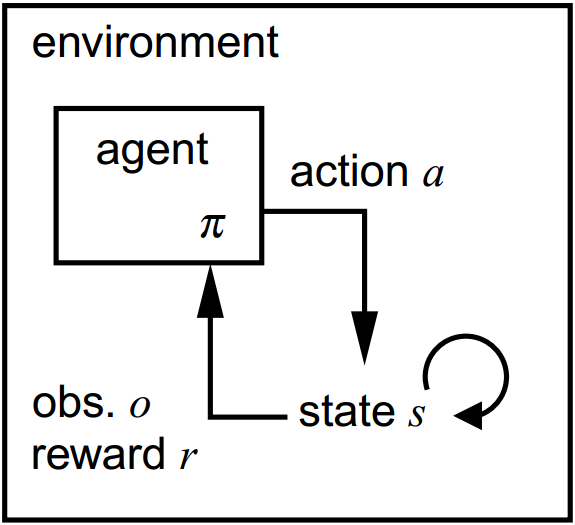
\includegraphics[width=3.5cm]{figures/POMDP-schema.png}
            \end{figure}
        \end{column}
    \end{columns}
    
\end{frame}

{\putbg
\section{The problem}
}

\begin{frame}{Example of a power line in medium voltage}
    \vspace{-5pt}
    \begin{figure}
        \centering
        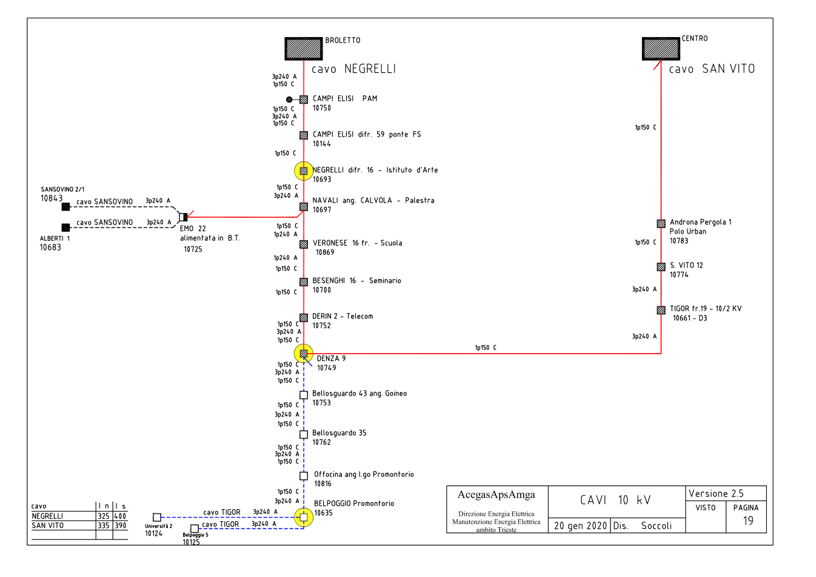
\includegraphics[width=0.8\textwidth]{figures/Rete_TS_1.png}
    \end{figure}
\end{frame}

\begin{frame}{The energy flow in the standard set-up}
    \vspace{-5pt}
    \begin{figure}
        \centering
        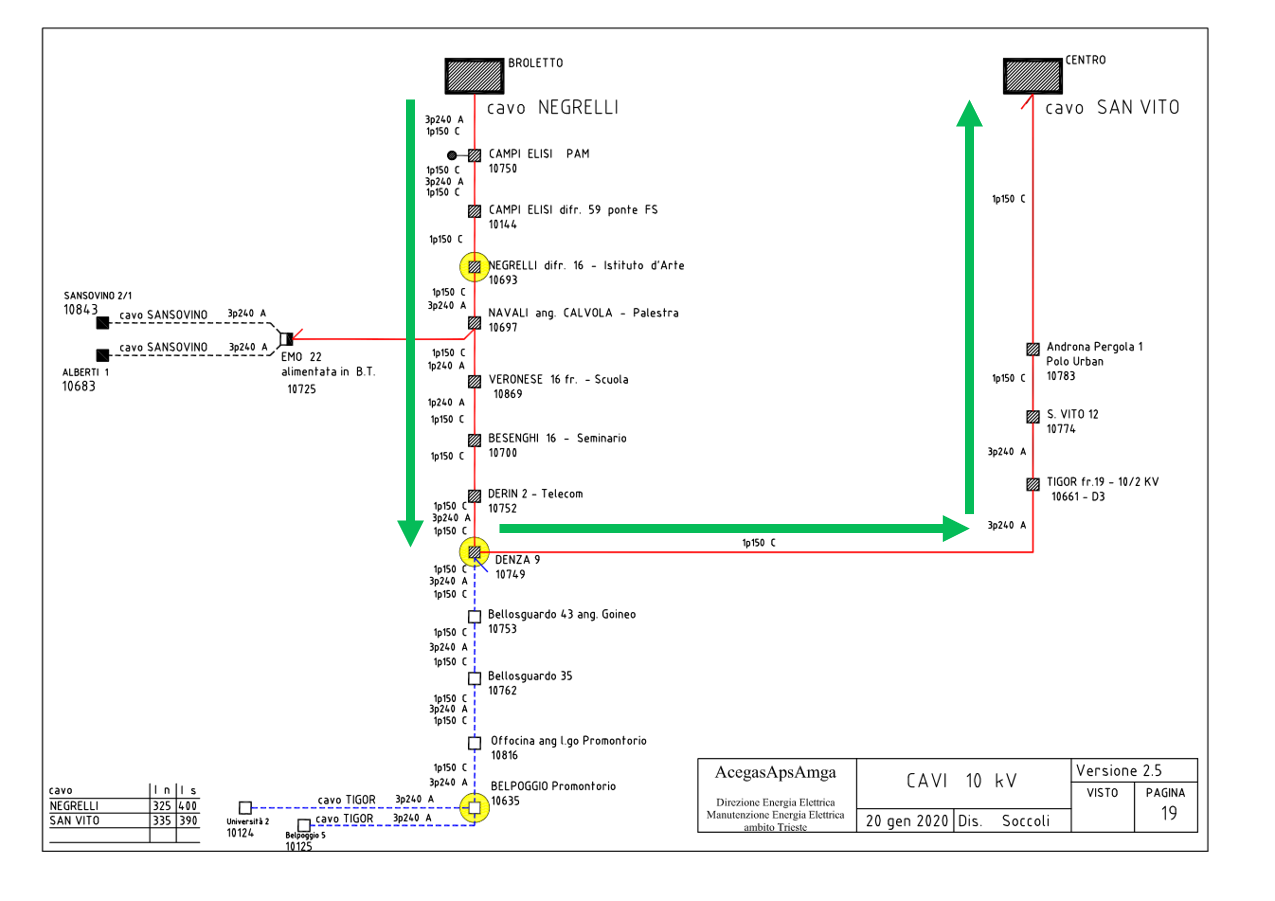
\includegraphics[width=0.8\textwidth]{figures/Rete_TS_2.png}
    \end{figure}
\end{frame}

\begin{frame}{Failure scenario}
    \vspace{-5pt}
    \begin{figure}
        \centering
        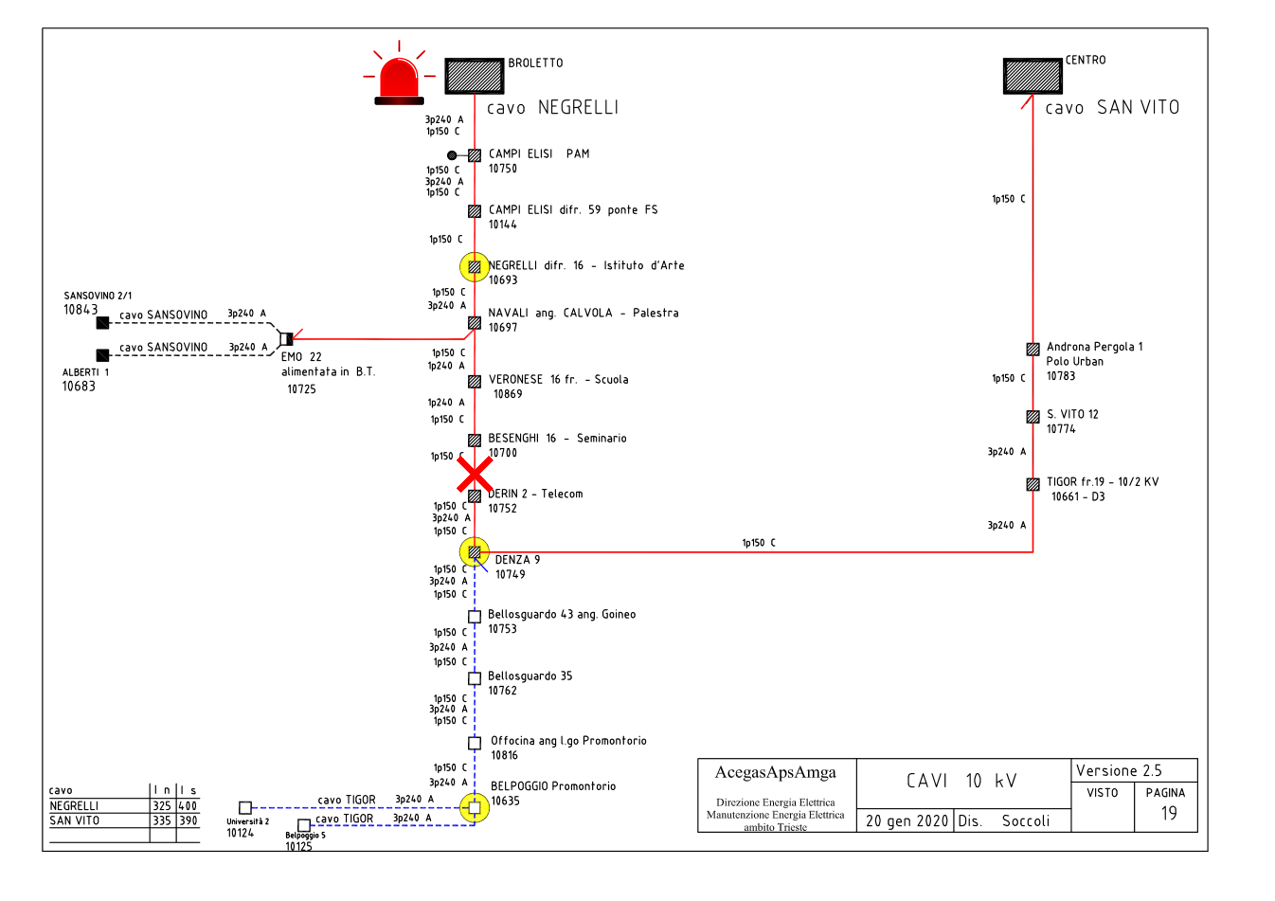
\includegraphics[width=0.8\textwidth]{figures/Rete_TS_3.png}
    \end{figure}
\end{frame}

\begin{frame}{Failure scenario}
    \vspace{-5pt}
    \begin{figure}
        \centering
        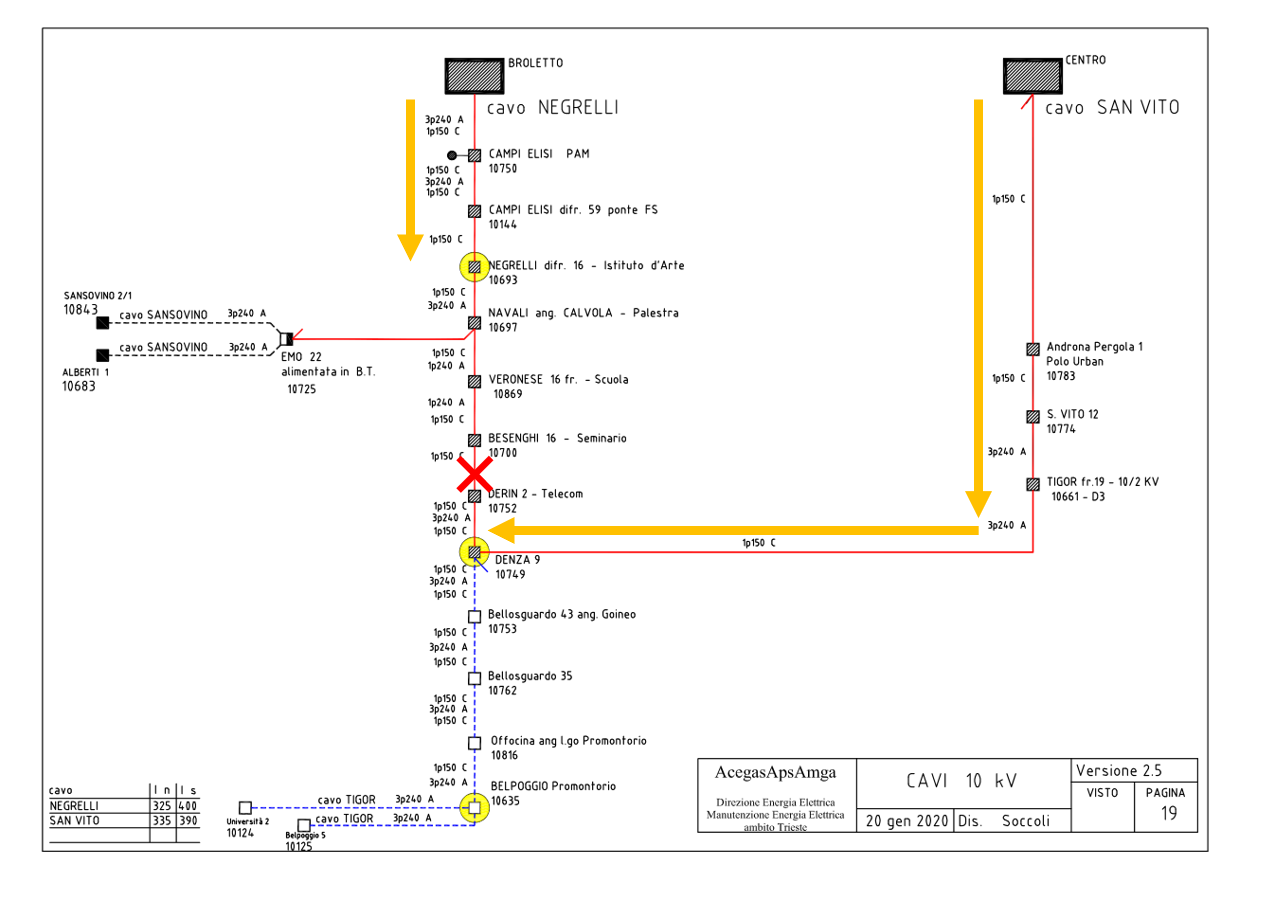
\includegraphics[width=0.8\textwidth]{figures/Rete_TS_4.png}
    \end{figure}
\end{frame}

\begin{frame}{Failure scenario}
    \vspace{-5pt}
    \begin{figure}
        \centering
        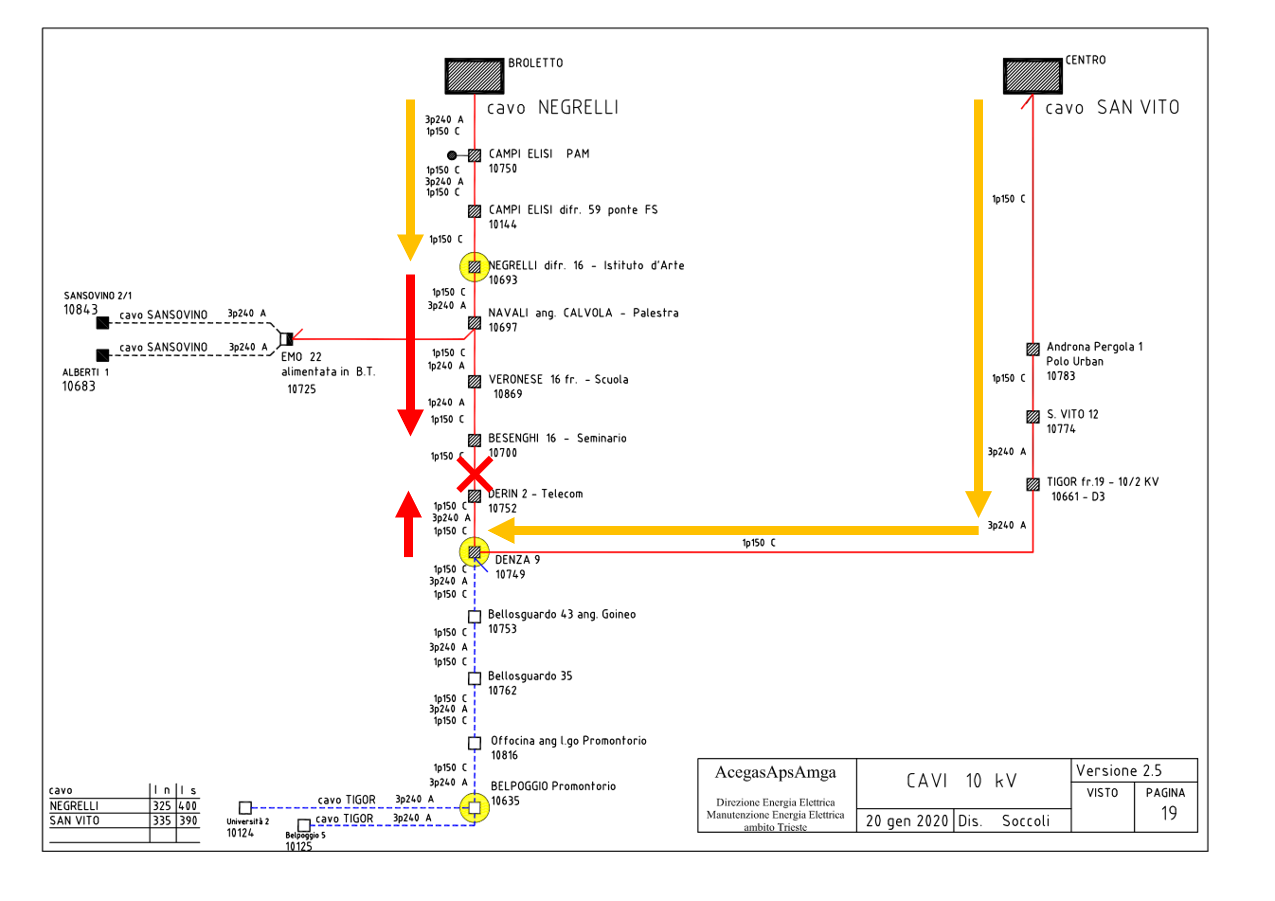
\includegraphics[width=0.8\textwidth]{figures/Rete_TS_5.png}
    \end{figure}
\end{frame}

{\putbg
\section{The mathematical framework}
}

\begin{frame}{The POMDP}

    Since we don't know where the fault is, we have a problem with \textbf{partially observable states}, so we will use a \alert{partially observable Markov decision process (POMDP)}.

    We are given a set of disconnected substations, $\mathcal C$, between two remotely controlled substations. In our problem $|\mathcal C| < 20$.

    \begin{itemize}
        \item[\alert{$\bullet$}] The \alert{state} is
        \begin{equation*}
            s = (x_g, v_k, \{v\})
        \end{equation*}
        \begin{itemize}
            \item[\alert{-}] $x_g$ is the position of the fault (\textbf{hidden});\\
            \item[\alert{-}] $v_k \in \mathcal C$ is the substation in which the technician is (\textbf{observable});\\
            \item[\alert{-}] $\{v\}$ is the set of the still disconnected substations after the technician operates in the current substation $v_k$ (\textbf{observable}).
        \end{itemize}
        \medskip
        
        \item[\alert{$\bullet$}] The \alert{observation} is
        \begin{equation*}
            o = (v_k, \{v\})
        \end{equation*}
        We define it as a function of $s$: $o(s): s = (x_g, o ) \mapsto o$.
    \end{itemize}
\end{frame}

\begin{frame}{The POMDP}

    \begin{itemize}
        \item[\alert{$\bullet$}] The \alert{action} is the choice of the specific substation the technician will visit as the next step, so $a \in \mathcal C$. Actually, since we visit only disconnected substations, we have that $a \in \{v\}$ if we are in state $s = (x_g, v_k, \{v\})$.
        \begin{equation*}
            a \in \mathcal A \big( s = (x_g, v_k, \{v\}) \big) = \{v\}
        \end{equation*}
        With every action, we visit a substation and we reconnect it (if lucky, we can reconnect half of the substations). We are therefore positive that the process terminates.
        
        \item[\alert{$\bullet$}] The \alert{next state} is
        \begin{equation*}
            s' = (x_g, v_{k+1} = a, \{v'\})
        \end{equation*}
        where $\{v'\}$ is the set of disconnected substations after the technician operates in substation $v_{k+1}$. We have that the set of disconnected substations decreases after each action, so $\{v'\} \subseteq \{v\} \backslash a$.
    \end{itemize}
    
\end{frame}

\begin{frame}{The POMDP}

    \begin{itemize}
        \item[\alert{$\bullet$}] The \alert{expected cost} is the time (\textit{in seconds}) of going in a certain substation multiplied by the number of disconnected users.
        \medskip
        
        $d_{v_k, v_{k+1}}$ $\longrightarrow$ time \textit{in seconds} to go from the substation $v_k$ to the next substation $v_{k+1}$.
        \medskip
        
        $n_{k} = \sum_{v \in \{v\}} u_v$ $\longrightarrow$ number of users still disconnected \underline{before} operating in the substation $v_{k+1}$, where $u_v$ is the number of users underneath substation $v$.
        \medskip
        
        \begin{equation*}
            r \Big( s = (x_g, v_k, \{v\}), a \Big) = d_{v_k, a} \cdot n_{k} = d_{v_k, a} \cdot \sum_{v \in \{v\}} u_v
        \end{equation*}
        \smallskip

        For now, in the cost we will ignore the cost of establishing if the fault is before or after the substation in which the technician is, which is complicated and might rise the total cost significantly.
    \end{itemize}
    
\end{frame}

\begin{frame}{The POMDP}
    When the fault occurs, the technician can be everywhere: at home if it is the middle of the night, at the company, be around, etc. So we introduce an extra dummy substation, called substation $0$, that is the position of the technician when the fault occurs.\\
    So the \alert{initial state} is always
    \begin{equation*}
        s_0 = ( \, x_g, o_0 = (0, \mathcal C) \, )
    \end{equation*}
    thus we have $|x_g| = 2 |\mathcal C| + 1$ initial states, one for every possible position of the fault. 
    
    \bigskip
    
    Instead, the \alert{terminal state} is of the form
    \begin{equation*}
        s_t = (x_g, v_k, \varnothing)
    \end{equation*}
    where we have that, if the fault is on a cable, $v_k$ will be one of the two substations at the ends of that faulty cable, so we would have two terminal states, while if the fault is in a substation, $v_k$ would be that exact substation, so the terminal state would be only one.

\end{frame}

\begin{frame}{Example}

    \begin{textblock*}{\textwidth}[0,0](0in,0in)
        \centering
        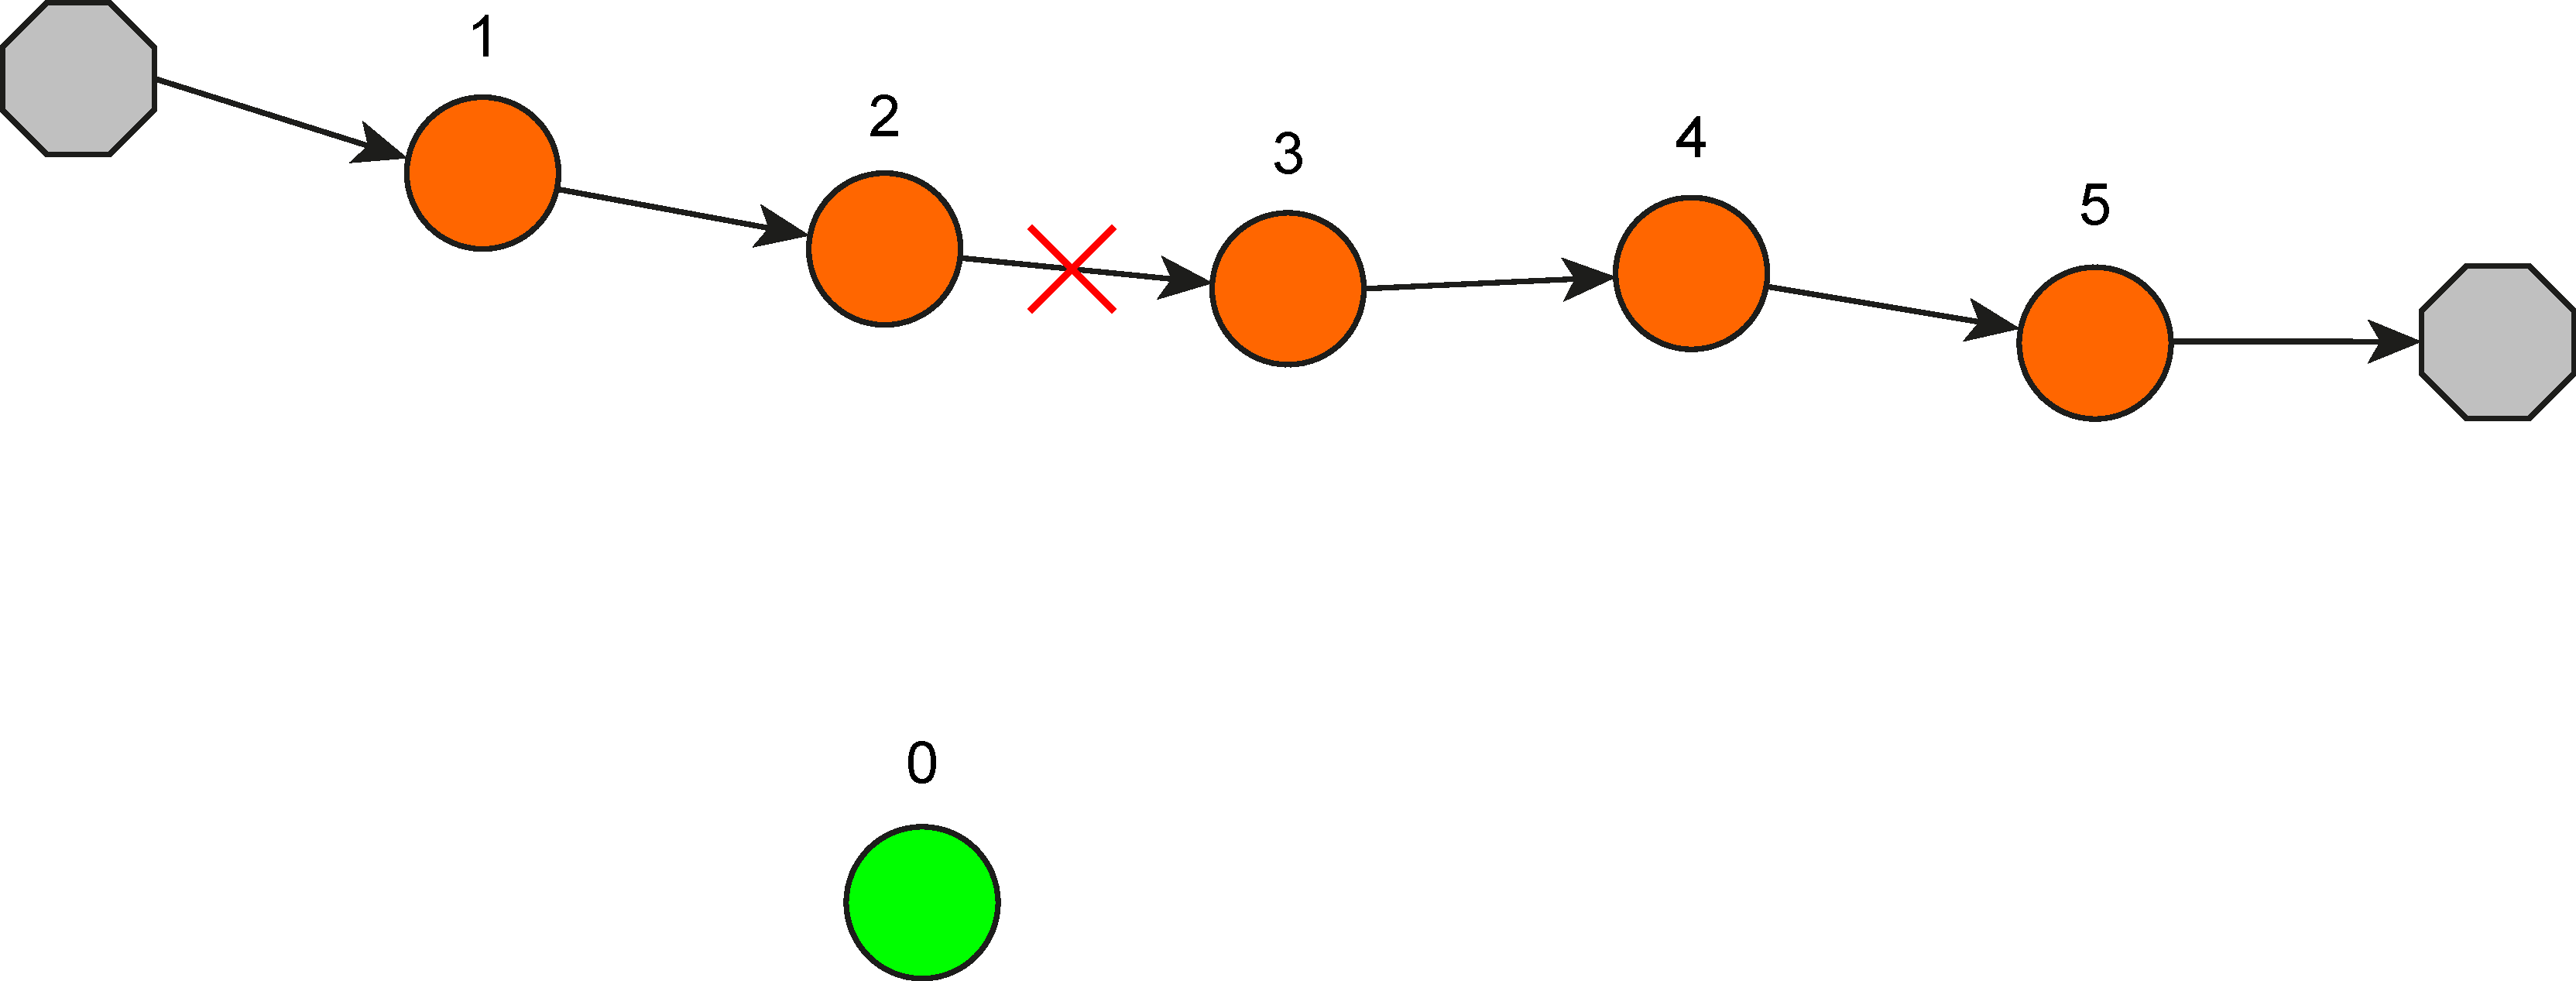
\includegraphics[width=0.8\textwidth]{figures/MDP_0.pdf}
    \end{textblock*}
    
    \vspace*{5cm}
    A fault has occurred in $2 \mhyphen 3$. We are in substation $0$ and all the substations are disconnected (orange). Initial state: $s_0 = (2 \mhyphen 3, 0, \mathcal C = \{1,2,3,4,5\})$.
    
\end{frame}

\begin{frame}{Example}

    \begin{textblock*}{\textwidth}[0,0](0in,0in)
        \centering
        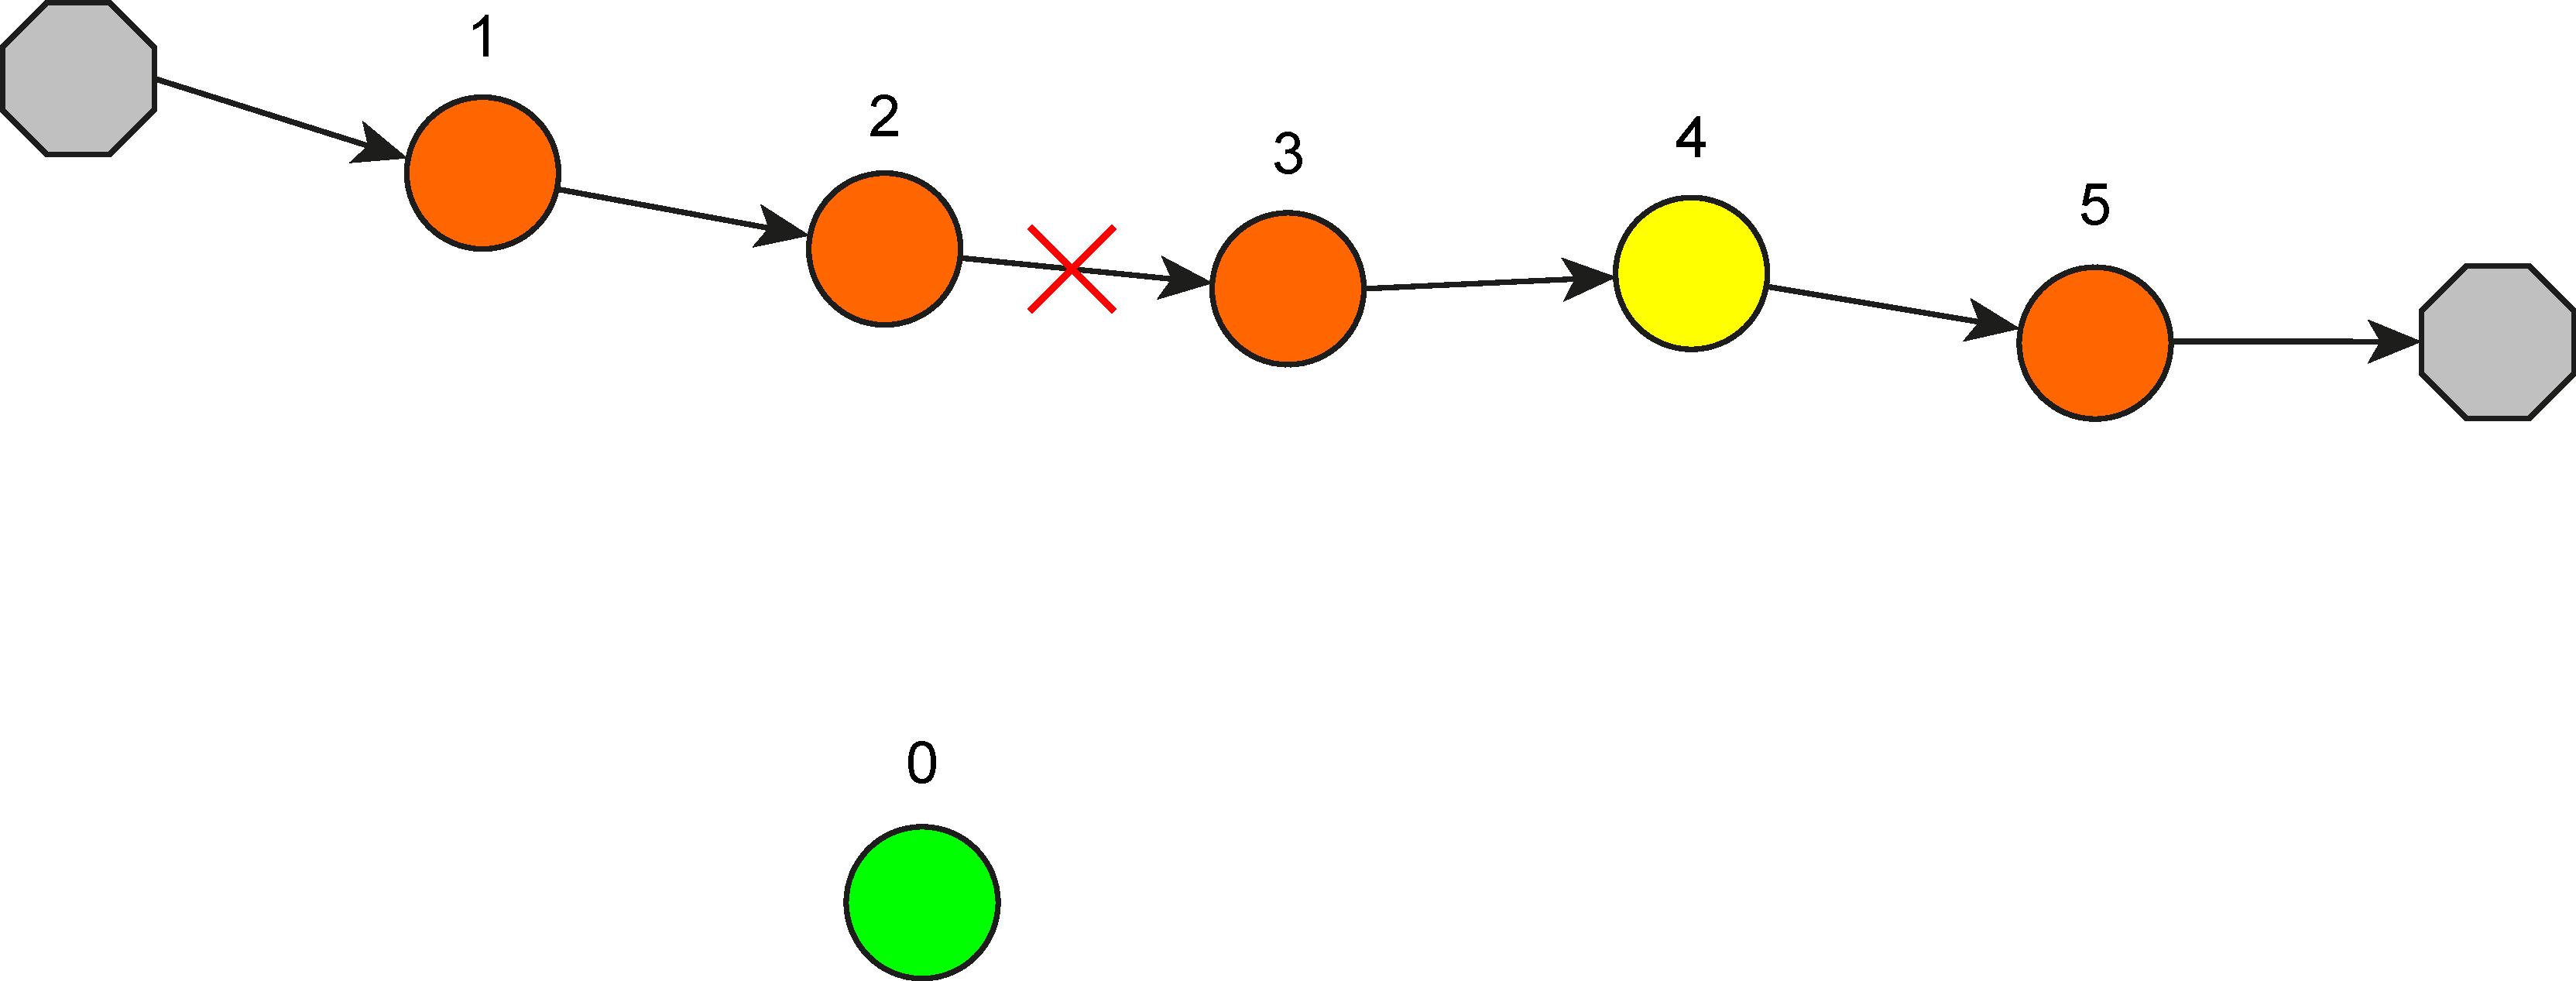
\includegraphics[width=0.8\textwidth]{figures/MDP_1.pdf}
    \end{textblock*}
    
    \vspace*{5cm}
    We visit substation $4$ (yellow). Action: $a_0 = 4$.
    
\end{frame}

\begin{frame}{Example}

    \begin{textblock*}{\textwidth}[0,0](0in,0in)
        \centering
        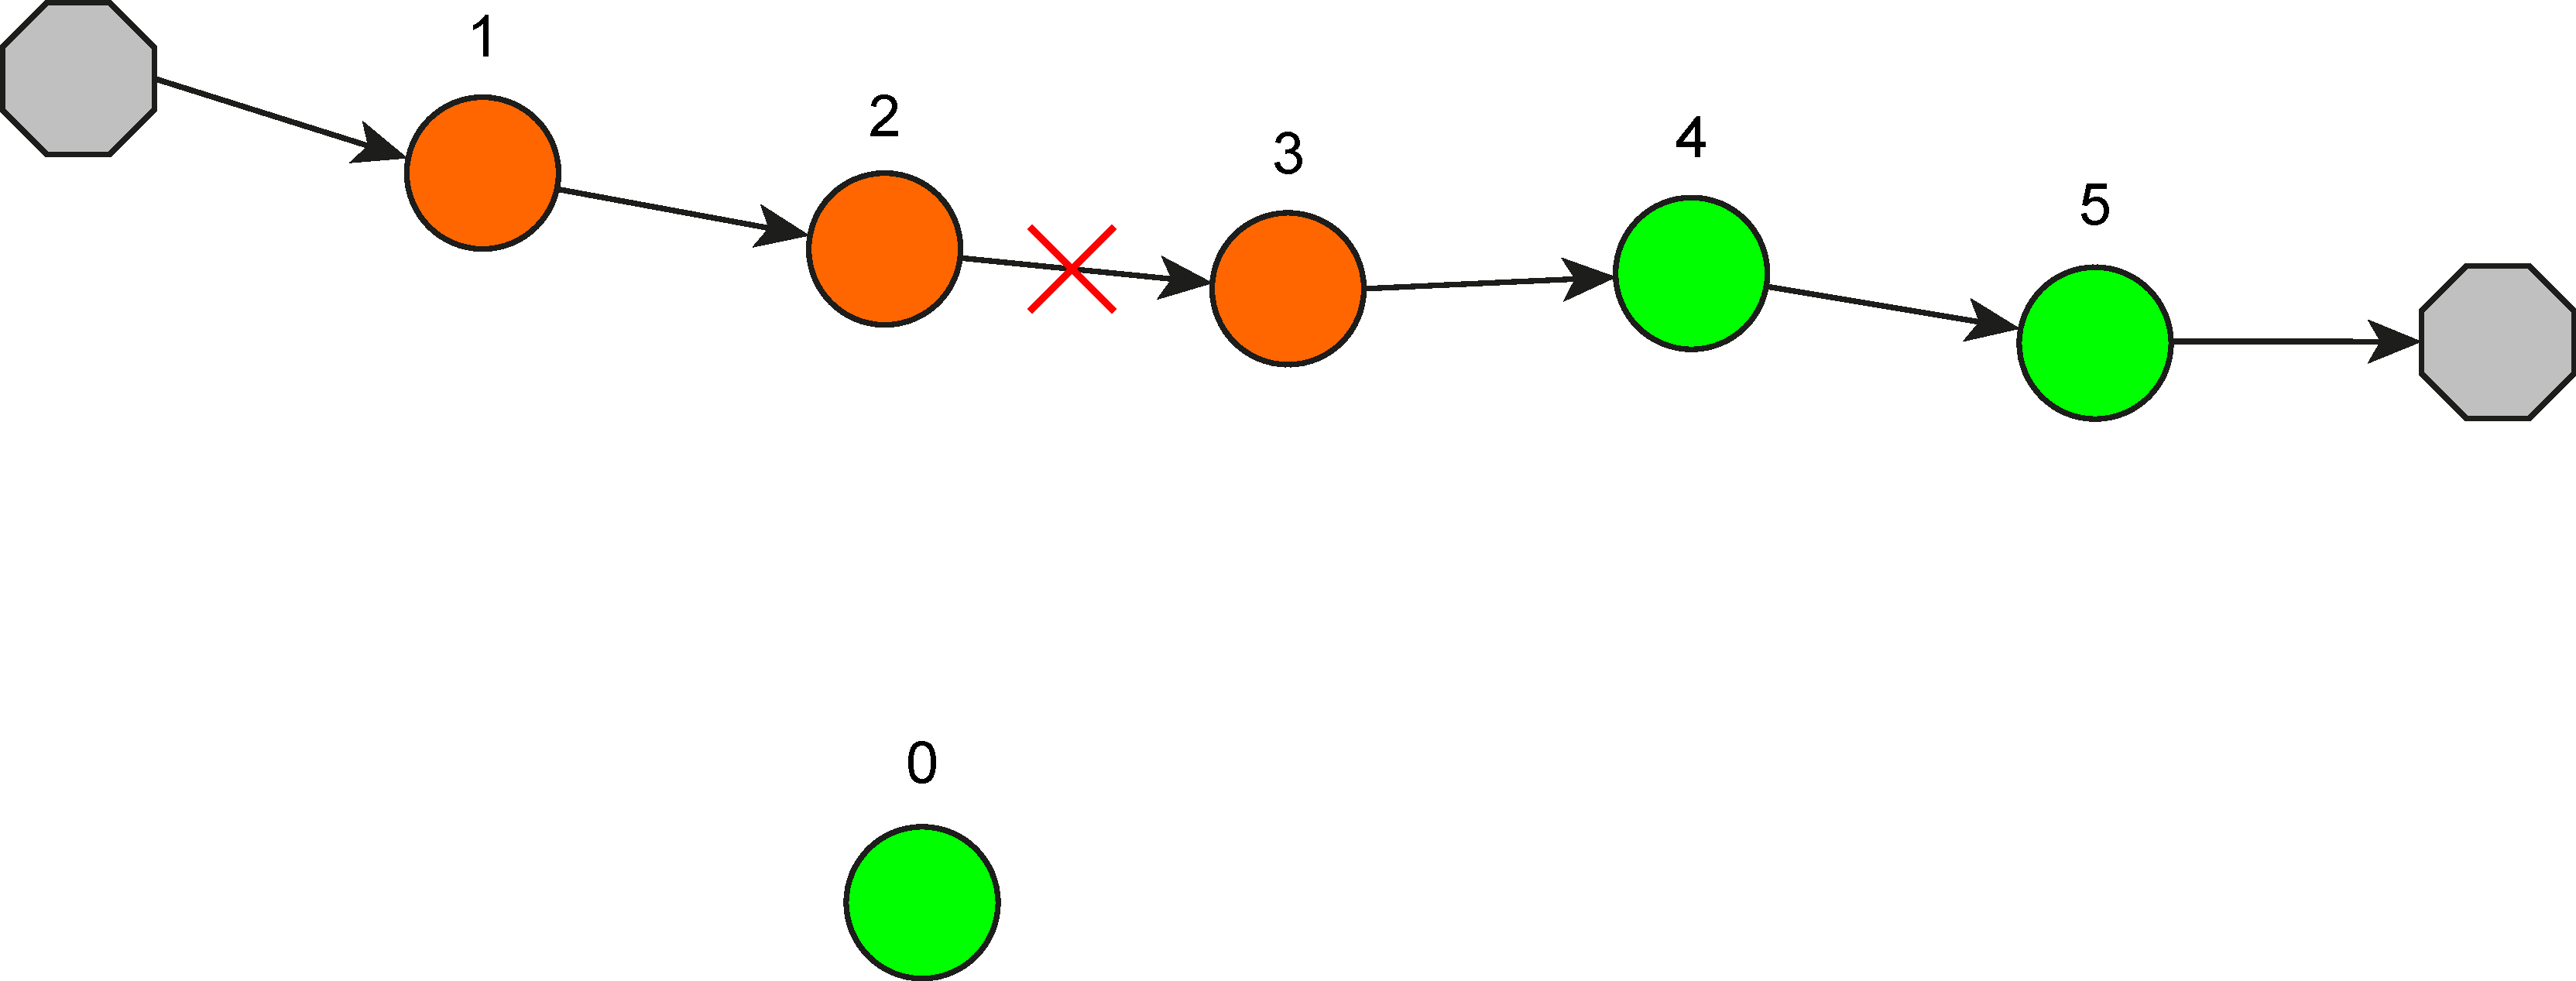
\includegraphics[width=0.8\textwidth]{figures/MDP_2.pdf}
    \end{textblock*}
    
    \vspace*{5cm}
    We reconnect substations $4$ and $5$ (green). State: $s_1 = (2 \mhyphen 3, 4, \{1,2,3\})$.
    
\end{frame}

\begin{frame}{Example}

    \begin{textblock*}{\textwidth}[0,0](0in,0in)
        \centering
        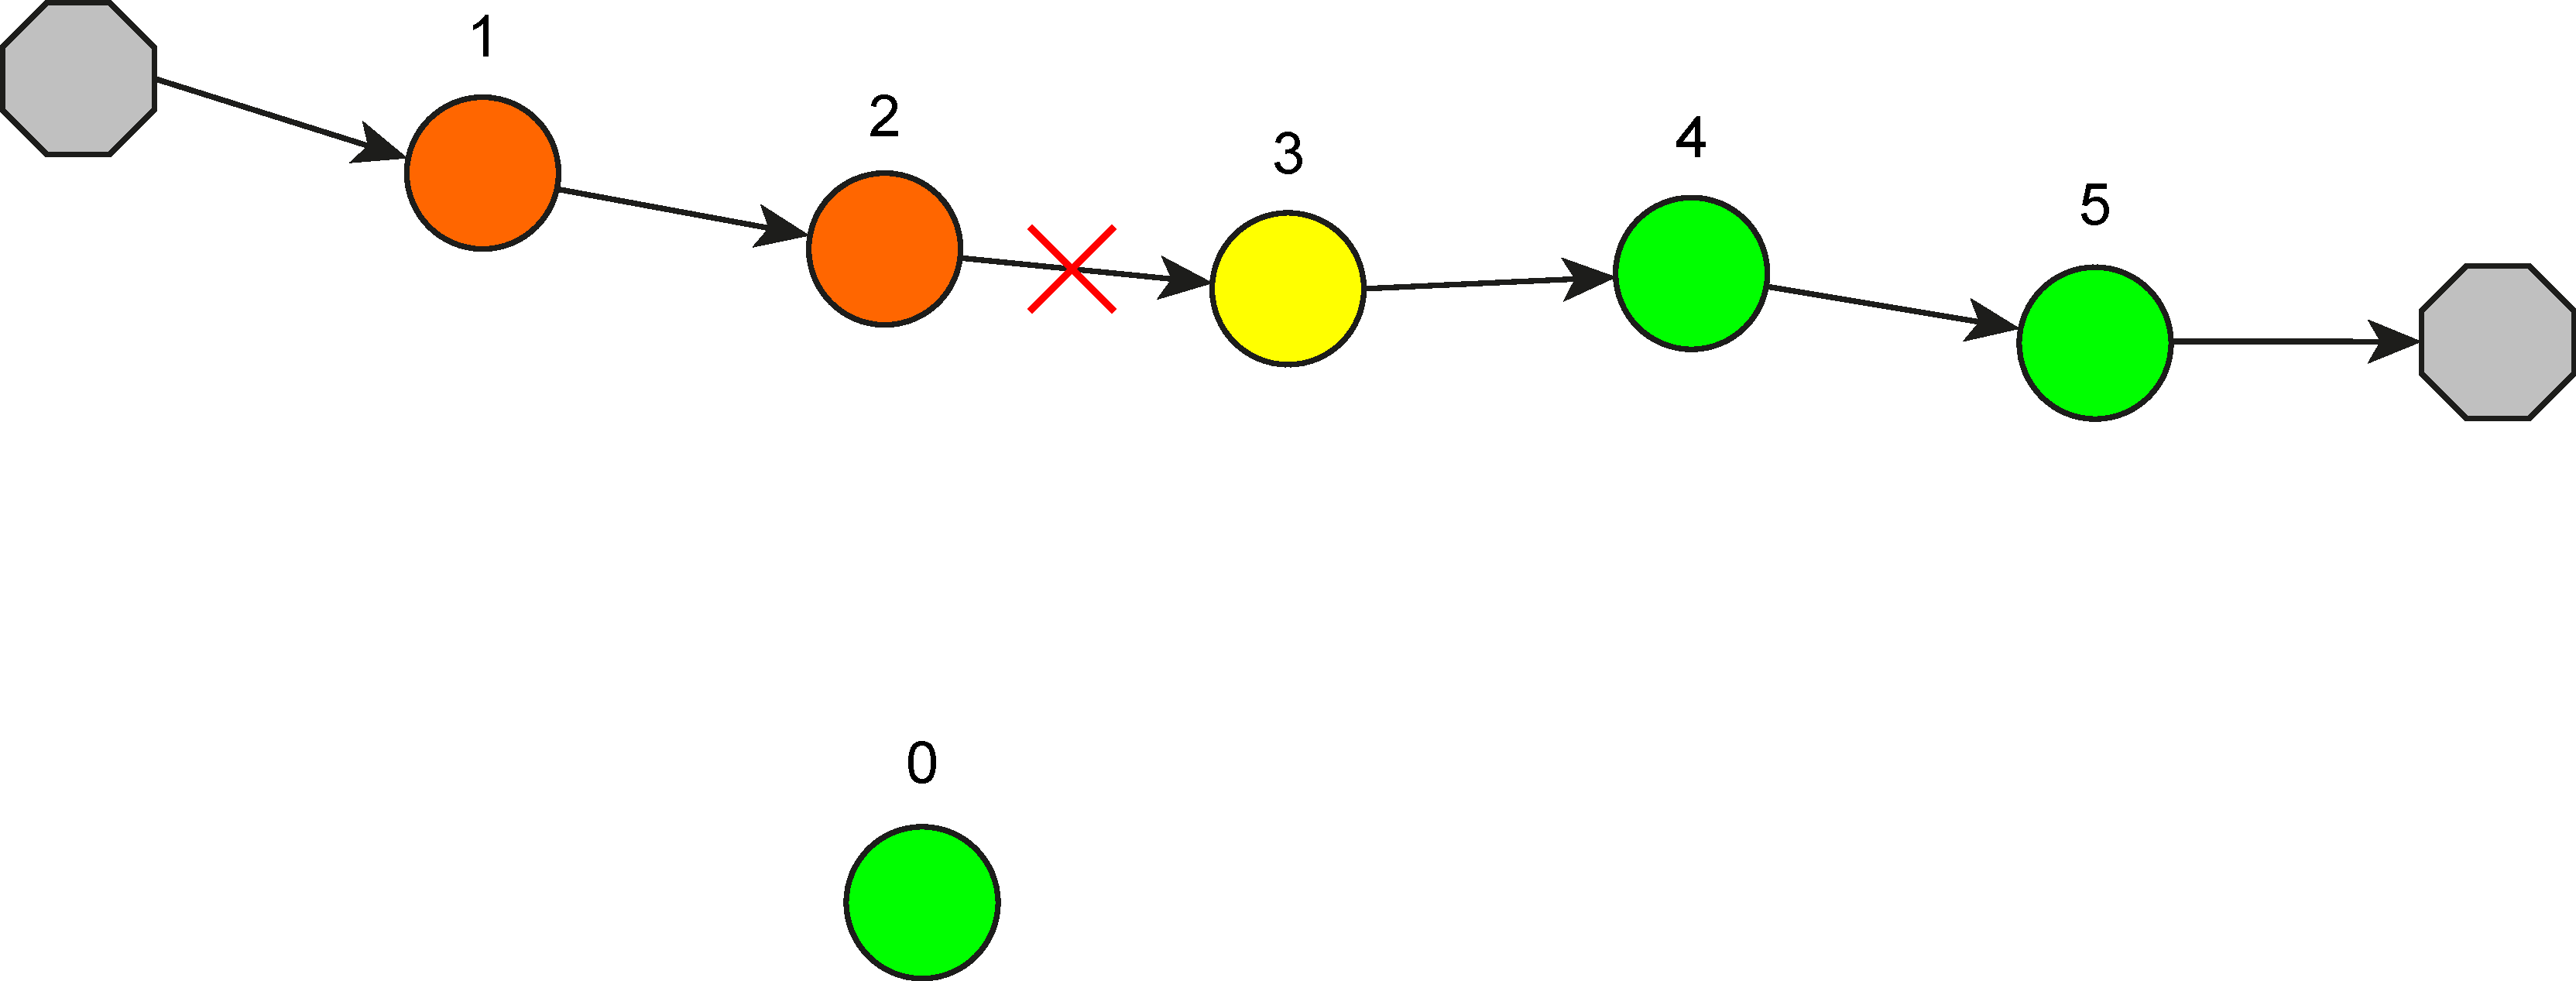
\includegraphics[width=0.8\textwidth]{figures/MDP_3.pdf}
    \end{textblock*}
    
    \vspace*{5cm}
    We visit substation $3$ (yellow). Action: $a_1 = 3$.
    
\end{frame}

\begin{frame}{Example}

    \begin{textblock*}{\textwidth}[0,0](0in,0in)
        \centering
        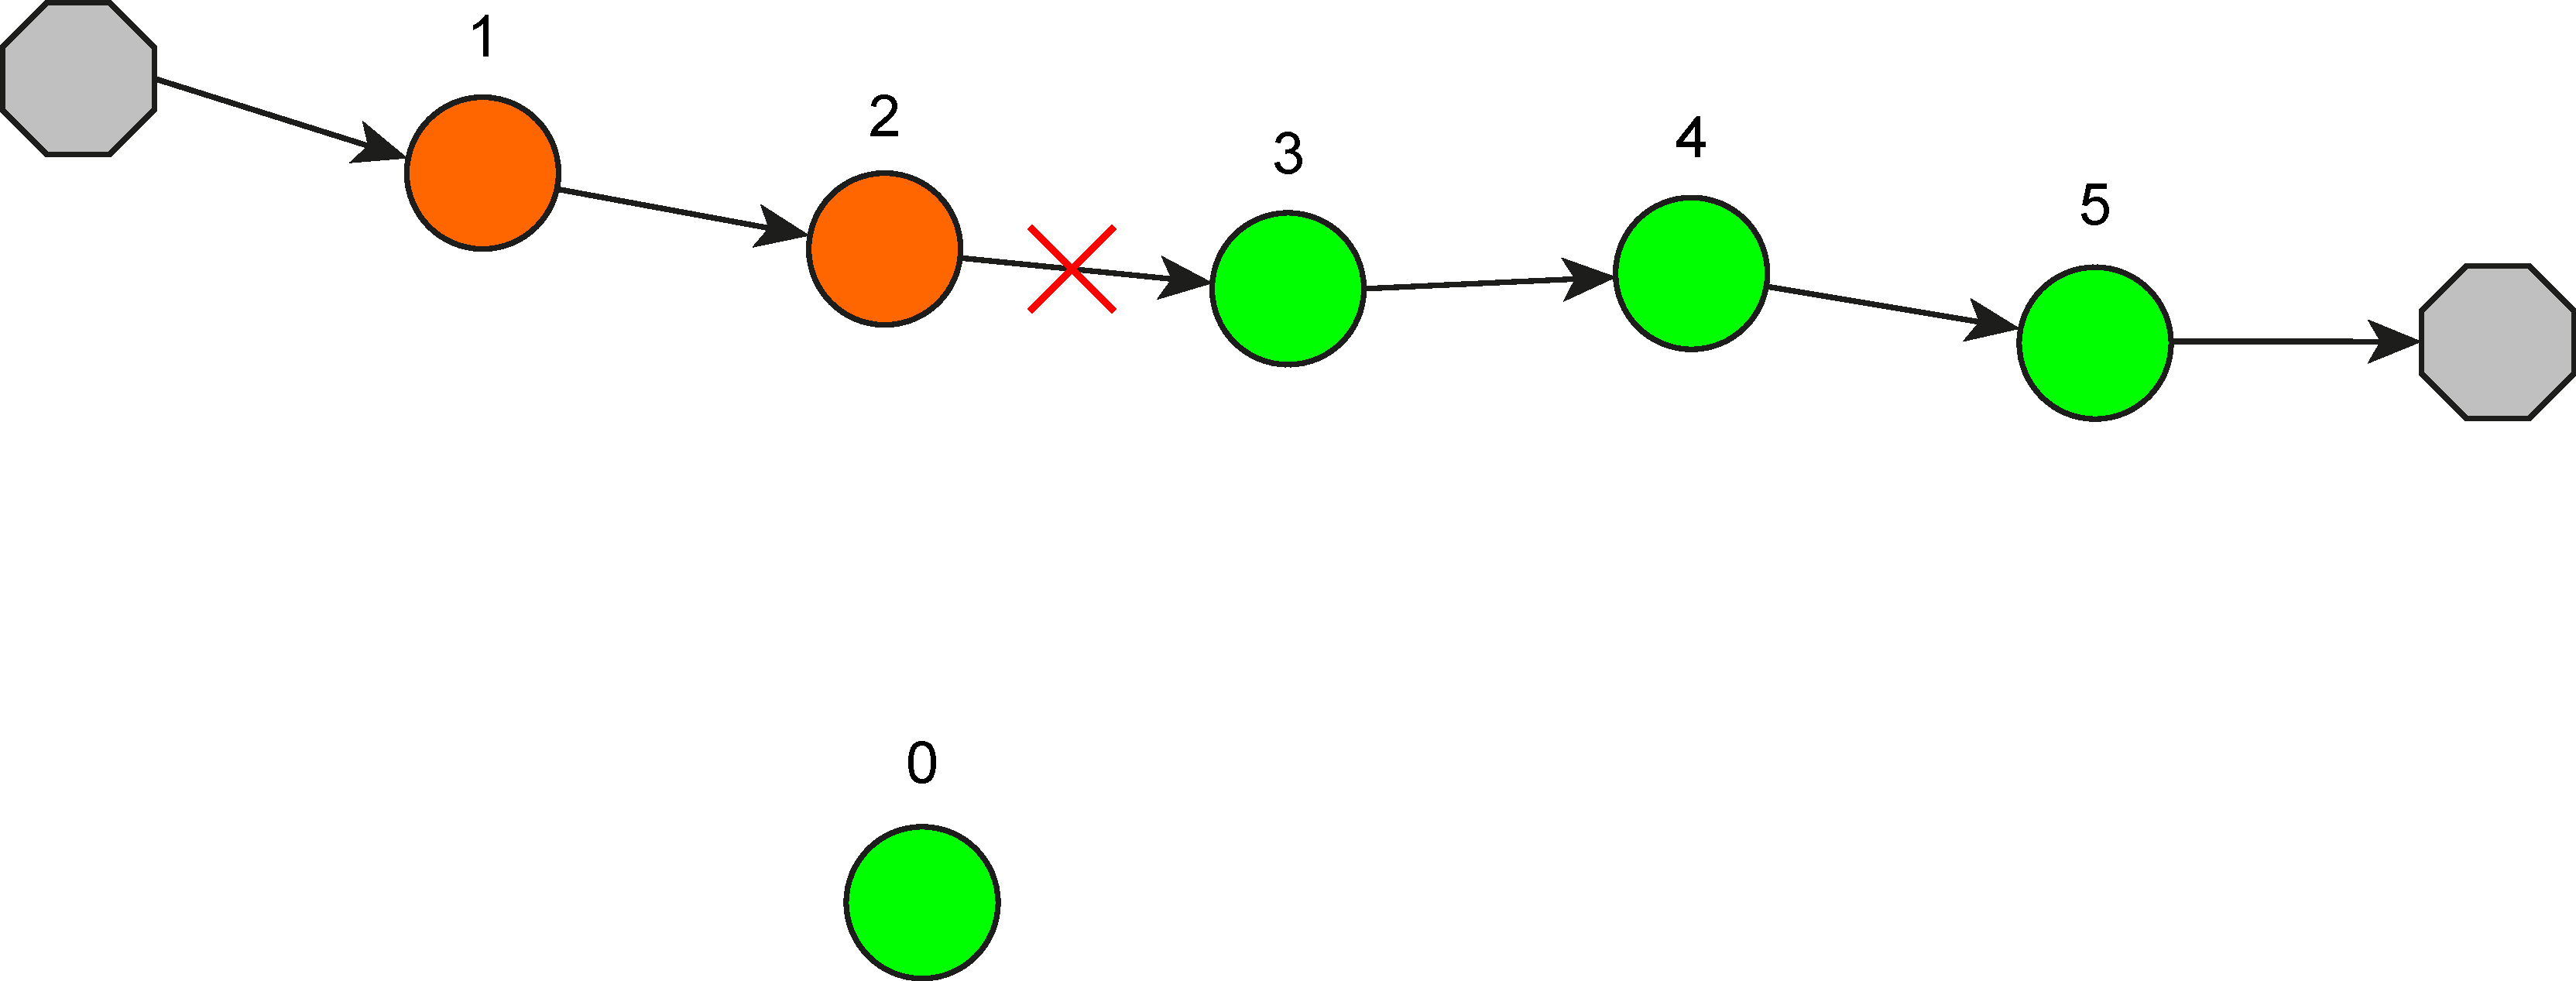
\includegraphics[width=0.8\textwidth]{figures/MDP_4.pdf}
    \end{textblock*}
    
    \vspace*{5cm}
    We reconnect substation $3$ (green). State: $s_2 = (2 \mhyphen 3, 3, \{1,2\})$.
    
\end{frame}

\begin{frame}{Example}

    \begin{textblock*}{\textwidth}[0,0](0in,0in)
        \centering
        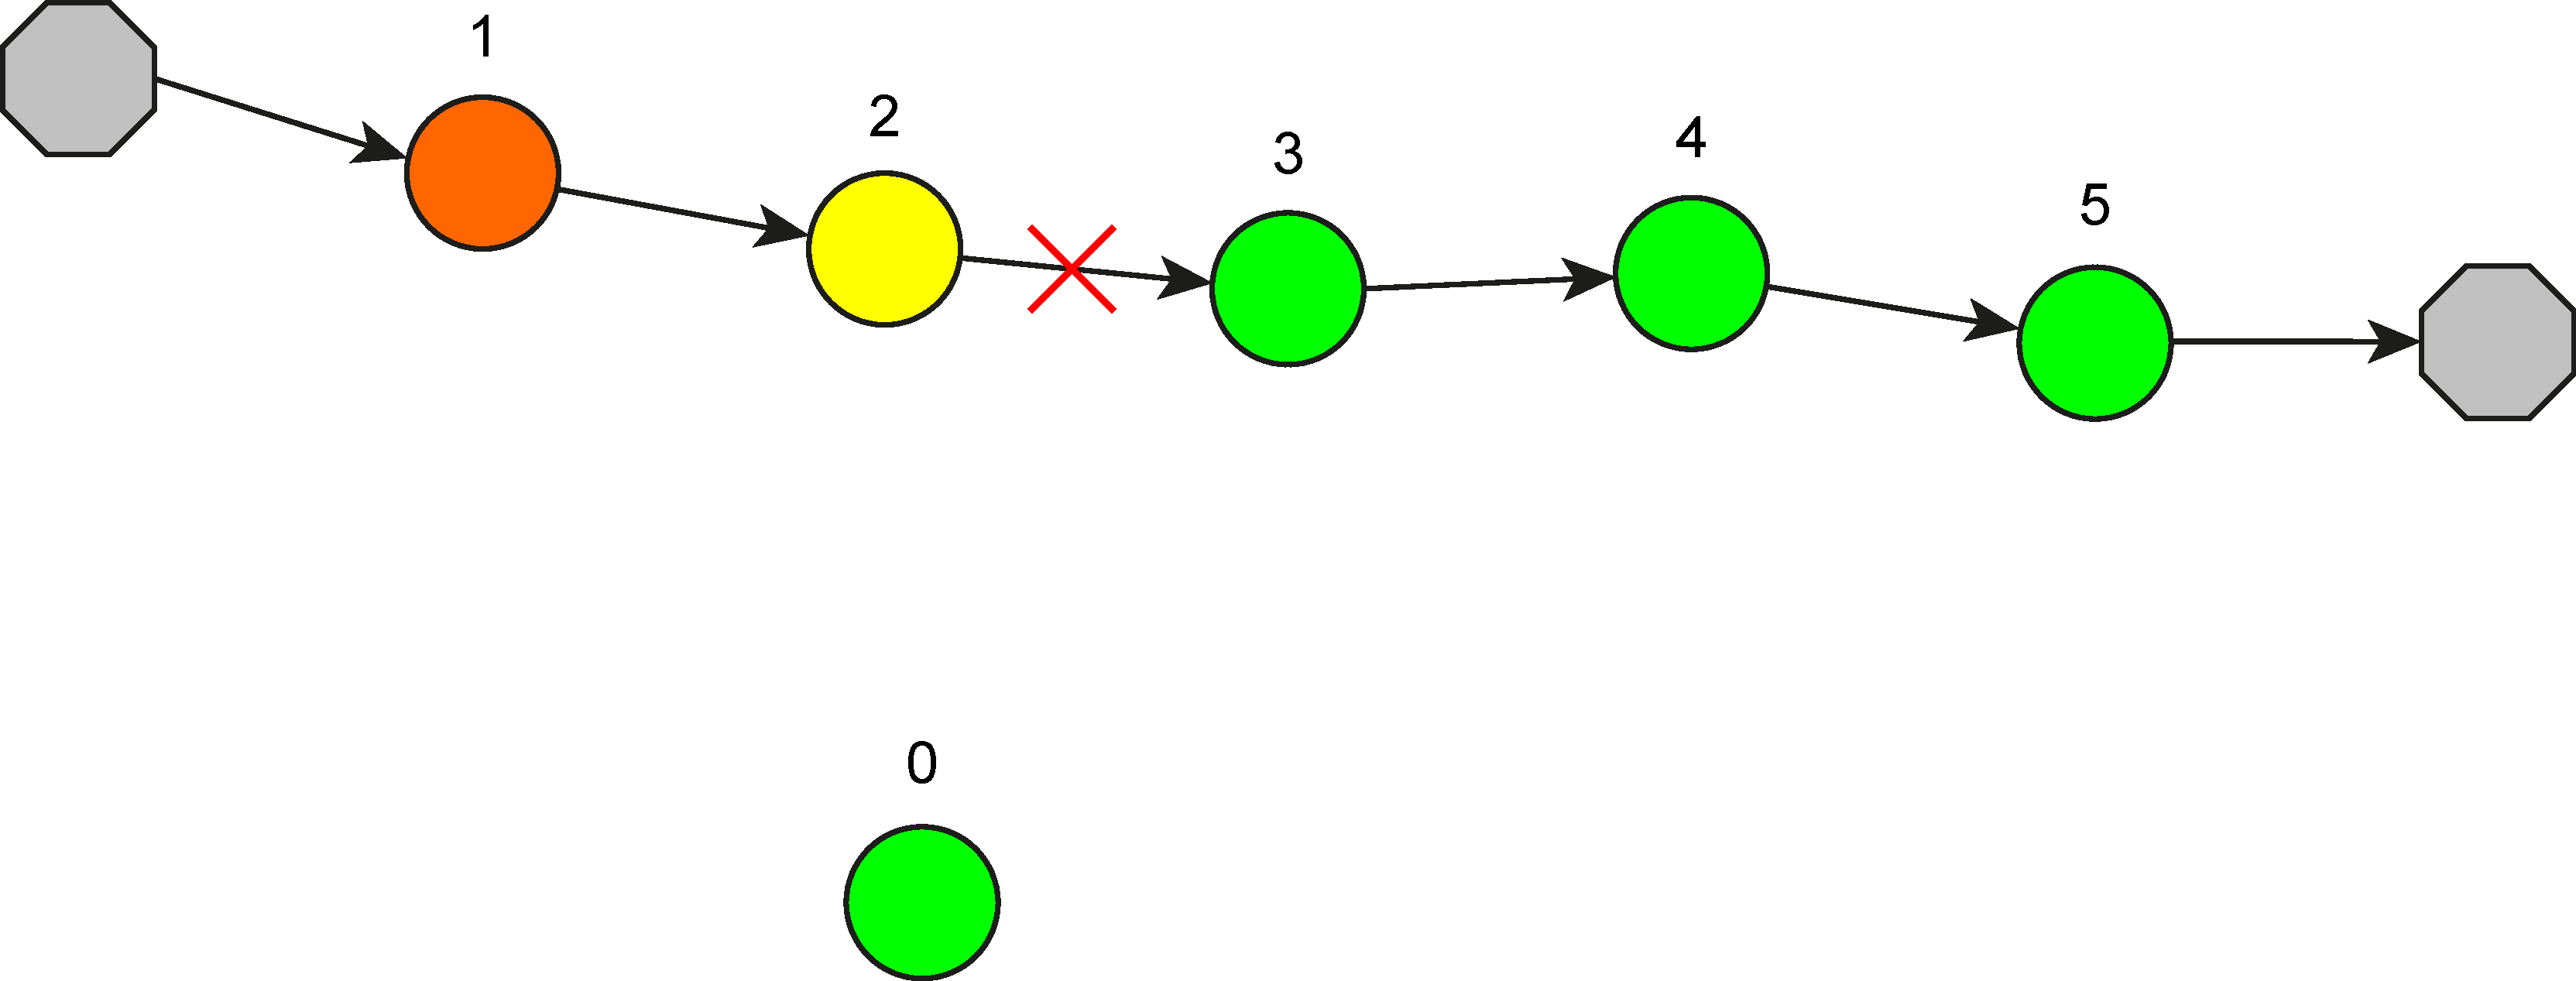
\includegraphics[width=0.8\textwidth]{figures/MDP_5.pdf}
    \end{textblock*}
    
    \vspace*{5cm}
    We visit substation $2$ (yellow). Action: $a_2 = 2$.
    
\end{frame}

\begin{frame}{Example}

    \begin{textblock*}{\textwidth}[0,0](0in,0in)
        \centering
        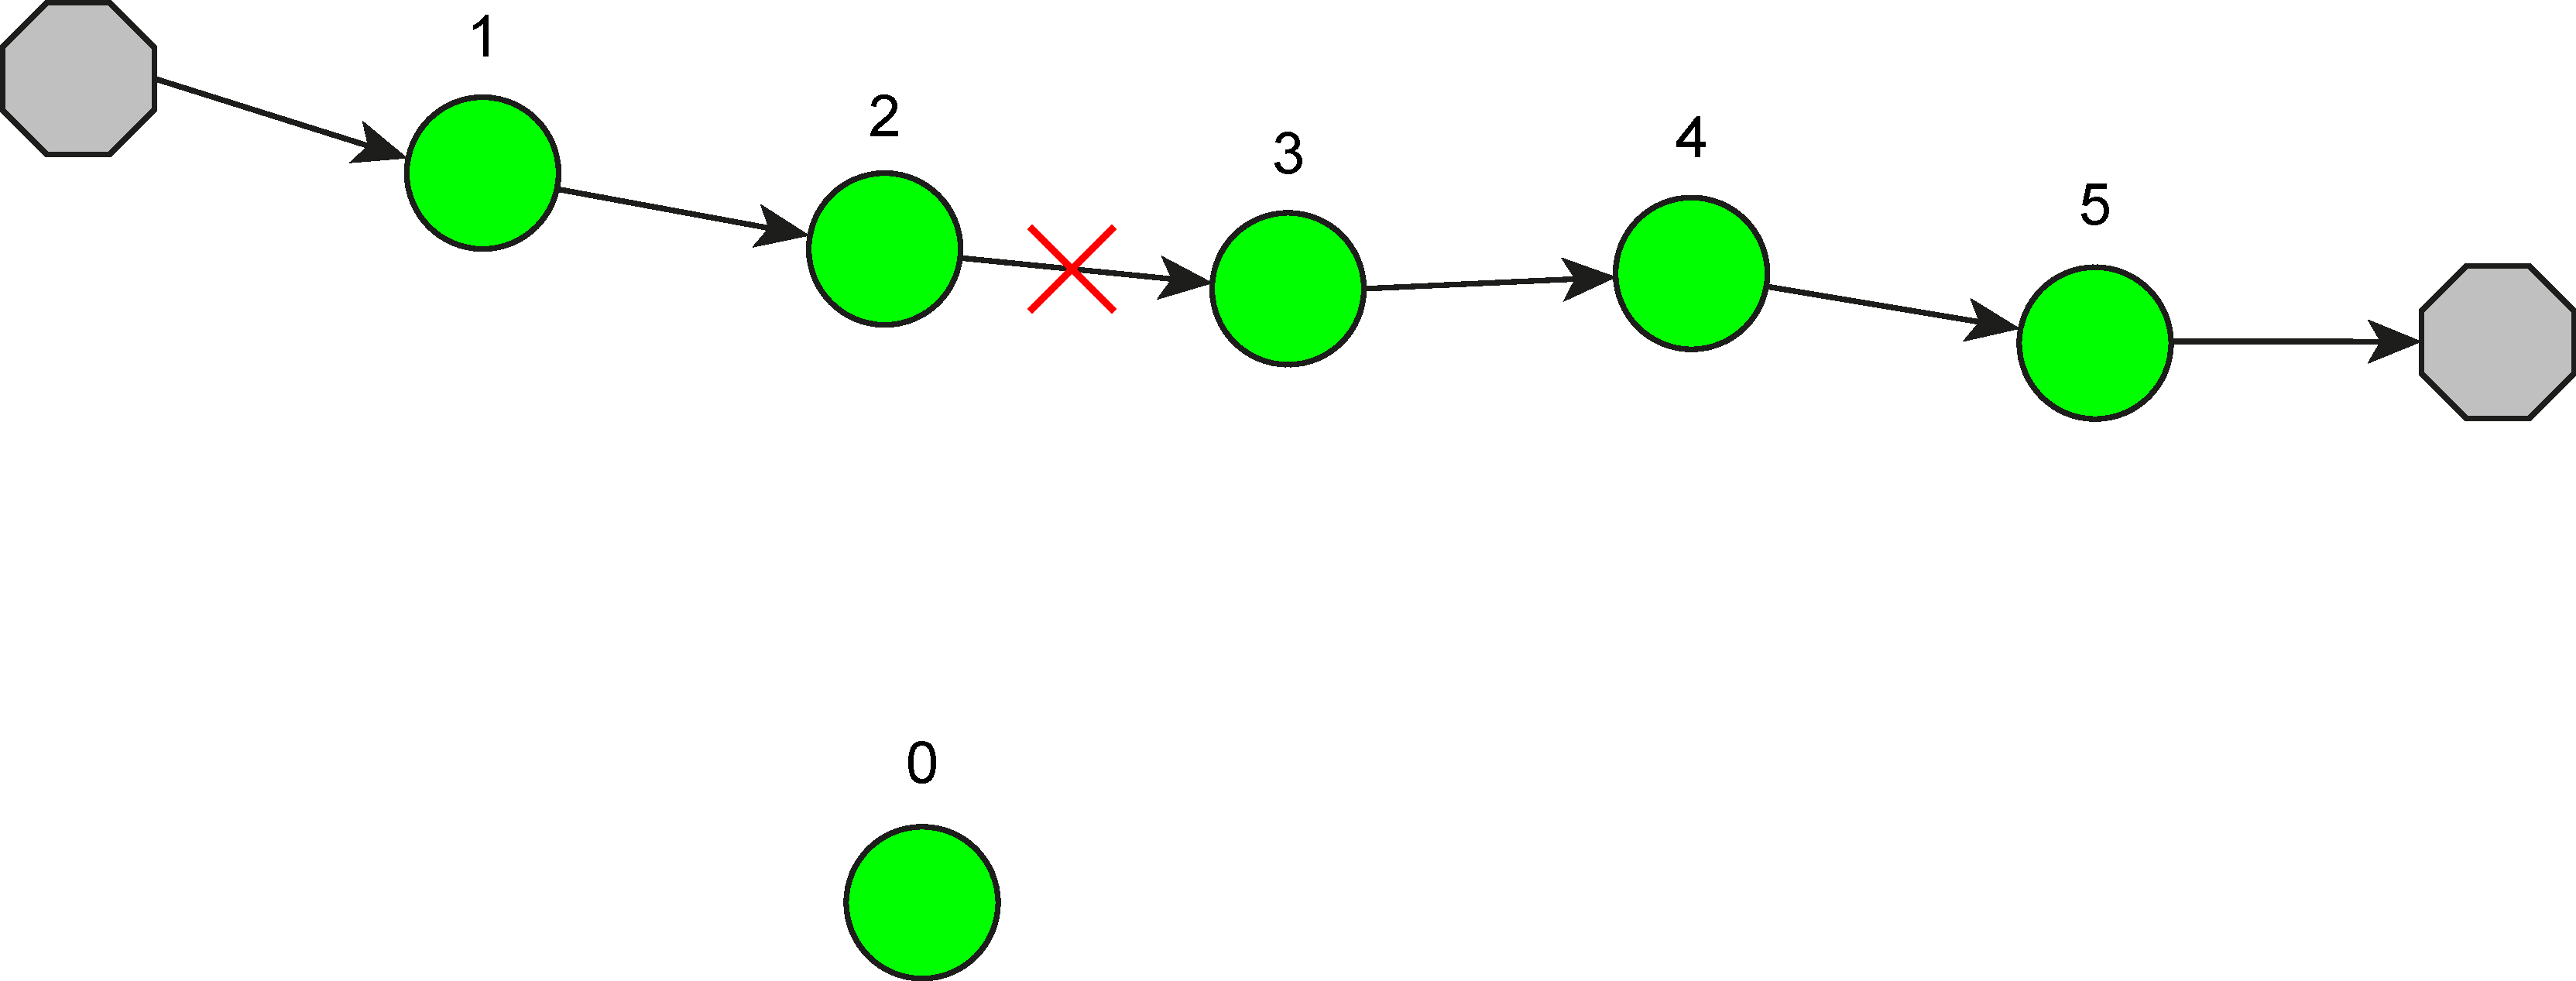
\includegraphics[width=0.8\textwidth]{figures/MDP_6.pdf}
    \end{textblock*}
    
    \vspace*{5cm}
    We reconnected substations $1$ and $2$ (green). All the substations are reconnected. Terminal state: $s_3 = (2 \mhyphen 3, 2, \varnothing)$.
    
\end{frame}

{\putbg
\section{The model}
}

\begin{frame}{The transition probability}
    
    The system is \alert{deterministic}, so, given an admissible action $a$, we will surely perform it and end up in the state to which that action leads.
    
    In our case we have that the \alert{transition probability} is equal to $1$ only when, starting from state $s = (x_g, v_k, \{v\})$, the new substation $v_{k+1}$ of the next state $s' = (x_g, v_{k+1}, \{v'\})$ is equal to the action $a \in \{v\}$ that we took:
    
    \begin{equation*}
        p(s' \mid s, a) = \mathbb I\big(s' = \sigma(s, a)\big) =
        \begin{cases}
            1 & \text{if } v_{k+1} = a \\
            0 & \text{if } v_{k+1} \neq a
        \end{cases} \,.
    \end{equation*}
    
\end{frame}

\begin{frame}{The policy}

    The \alert{policy} depends only on the observable states, so it doesn't know where the fault is. Let's define a parameterized policy using the \emph{soft-max (i.e., Boltzmann) distribution}:
    \begin{equation*}
        \pi \Big( a \;\big|\; o=(v_k, \{v\}); \boldsymbol \theta \Big) = \frac{e^{\theta_{o,a} }}{\sum_{b \in \{v\}} e^{\theta_{o,b} }} \,.
    \end{equation*}
    where $\boldsymbol \theta$ are the parameters for each observation $o$ and action $a$:
    \begin{equation*}
        \boldsymbol \theta = (\theta_{o,a})_{o \in \mathcal O, a \in \mathcal A} = \begin{pmatrix}
        \theta_{o_1, a_1} & \cdots & \theta_{o_1, a_{|\mathcal C|}} \\
        \vdots            &                   & \vdots            \\
        \theta_{o_{|O|}, a_1} & \cdots &  \theta_{o_{|O|}, a_{|\mathcal C|}} \\
        \end{pmatrix} \, .
    \end{equation*}
    
    The policy cannot depend on the position of the failure, otherwise we would have automatically solved the problem: the solution would be to go in the substation in which the failure is or at the substations at the ends of the faulty electrical cable.
    
\end{frame}

\begin{frame}{The action value function $Q$}
    
    The \alert{action value function} or \alert{quality} of the state-action pair, thanks to the Bellman equation, is:
    \begin{equation*}
        Q_\pi(s,a) = \sum_{s'} p(s' | s,a) \left(r(s,a,s') + \sum_{a'} \pi(a'|o(s'); \boldsymbol \theta) Q_\pi(s',a') \right) \, .
    \end{equation*}
    
    Given that the state is $s = ( \, x_g, o = (v_k, \{v\}) \, )$, the action is $a \in \{v\}$ and the new state is $s' = \sigma(s,a) = ( \, x_g, o' = (v_{k+1}=a, \{v'\}) \, )$, it becomes:

    \begin{align*}
            Q_\pi(s,a) = \left(d_{v_k, a} \cdot n_{k} + \sum_{a' \in \{v'\}} \pi \Big( a' \big| o \big( \sigma(s,a) \big); \boldsymbol \theta \Big) \, Q \big( \sigma(s,a), a' \big) \right) \,.
    \end{align*}
    
\end{frame}

\begin{frame}{The $\eta$ function}

    We define $\rho_0(s')$ as the probability of starting in the state $s'$. In our case
    \begin{align*}
            \rho_0 \Big(s = ( x_g, v_k, \{v\}) \Big)
            &= \text{Pr}(x_g) \mathbb I(o(s) = o_0 = (0, \mathcal C)) \\
            &= \frac1{2|\mathcal C| + 1} \delta_{o(s), o_0} \, ;
    \end{align*}
    so $\rho_0$ is uniform in $x_g$ since it doesn't depend on the position of the fault.
    
    Besides, we define the average number of time steps that the agent spends in state $s'$ before the process dies as
    \begin{align*}
            \eta_\pi(s') &:= \rho_0(s') + \sum_s \eta_\pi(s) \sum_a \pi(a | o(s); \boldsymbol \theta) p(s' | s, a) \\
            &= \frac{1}{2|\mathcal C|+1} \delta_{o(s'), o_0} + \sum_{s \in \mathrm{pa}(s')} \eta_\pi(s) \pi(v_{k+1} | o(s); \boldsymbol \theta) \, ,
    \end{align*}
    
    \textbf{Notice} that the equations for both $Q_\pi$ and $\eta_\pi$ are \alert{linear systems}.

\end{frame}

\begin{frame}{The performance measure}
    
    Let's define the \alert{performance measure} $J_\pi(\boldsymbol \theta)$ as the sum of all the costs we incur, added up over time until the process is concluded:
    \begin{equation*}
            J_\pi (\boldsymbol \theta)
            = \mathbb E_\pi \left[ \sum_{t=0}^\infty r(s_t, a_t, s_{t+1}) \right]
            = \sum_{s \in \mathcal S} \rho_0(s) \sum_{a \in \mathcal A(s)} \pi_{\boldsymbol \theta} (a|o(s); \boldsymbol \theta) Q_{\pi_{\boldsymbol \theta}} (s,a)
    \end{equation*}
    
    Thanks to the \alert{policy gradient theorem} we have that
    \begin{equation*}
        \nabla_{\boldsymbol \theta} J_\pi (\boldsymbol \theta) = \sum_{s \in \mathcal S} \eta_{\pi_{\boldsymbol \theta}}(s) \sum_{a \in \mathcal A(s)} Q_{\pi_{\boldsymbol \theta}}(s,a) \nabla_{\boldsymbol \theta} \pi(a|o(s); \boldsymbol \theta) \, .
    \end{equation*}
    
    To optimize $J$ we perform a gradient descent on $\boldsymbol \theta$ with \emph{learning rate} $\alpha$:
    \begin{equation*}
        \boldsymbol \theta_{k+1} = \boldsymbol \theta_k - \alpha \nabla_{\boldsymbol \theta} J_\pi(\boldsymbol \theta_k) \, ,
    \end{equation*}
    
    %To find the quantities $\eta_\pi$ and $Q_\pi$, given a policy $\pi$, we need to solve two linear systems, and they must be re-computed at each operation.
    
\end{frame}

\begin{frame}[standout]
    
    \alert{Problem:} we can compute $Q_\pi$ and $\eta_\pi$ only if we know the position of the fault $x_g$!
    
\end{frame}
\stepcounter{framenumber}

\begin{frame}{Solution}
    
    Given the equation for the policy, we have that its derivative is
    \begin{equation*}
            \frac{\partial}{\partial \theta_{o',a'}} \pi \Big( a \;\big|\; o=(v_k, \{v\}); \boldsymbol \theta \Big) = \delta_{o',o} \left( \delta_{a',a} - \pi(a'|o; \boldsymbol \theta) \right) \, \pi(a|o; \boldsymbol \theta)
    \end{equation*}
    
    Therefore, the equation of the gradient becomes
    
    \begin{align*}
            \nabla_{\theta_{o',a'}} J_\pi (\boldsymbol \theta)
            &= \sum_{s \in \mathcal S} \eta_\pi(s) \sum_{a \in \mathcal A(s)} Q_\pi(s,a) \nabla_{\theta_{o',a'}} \pi(a|o(s); \boldsymbol \theta) \\
            &= \sum_s \eta_\pi(s) \sum_a Q_\pi(s,a) \delta_{o',o(s)} \Big( \big( \delta_{a',a} - \pi(a'|o(s); \boldsymbol \theta) \big) \, \pi(a|o(s); \boldsymbol \theta) \Big) \\
            &= \sum_{x_g} \eta_\pi((x_g, o')) \sum_a Q_\pi((x_g, o'),a) \left( \delta_{a,a'} - \pi(a'|o'; \boldsymbol \theta) \right) \, \pi(a|o'; \boldsymbol \theta) \, ,
    \end{align*}
    
    \alert{So, we sum all the values of the gradient that have the same observation but different $x_g$!}
    
\end{frame}

\begin{frame}{Idea of the algorithm}

    So we \textbf{parametrized the policy}, and we imposed that the parameters depend only on the observable variables. Now we try to find the best policy in this subspace in order to optimize the POMDP.
    
    \alert{We start from a certain policy}, for example \emph{random policy}, in which all the parameters $\theta$ are equal to $0$: $\boldsymbol \theta = \mathbf 0 = (0, 0, \ldots, 0)$, so that all actions have an equal probability of being selected
    \begin{equation*}
        \pi \left( a \;\big|\; o(s); \boldsymbol \theta \right) = \frac{e^{\theta}}{\sum_{b \in \{v\}} e^{\theta}} = \frac{e^{\theta}}{e^{\theta} \sum_{b \in \{v\}} 1 } = \frac1{ |\{v\}| } \, ,
    \end{equation*}
    
    Then we perform a \alert{step of gradient descent on the parameters $\boldsymbol \theta$ of the policy}. We compute the gradient using the previous formula: the gradients of the policy are simple computations, while to compute $Q_\pi$ and $\eta_\pi$ you have to solve the corresponding linear equations for the current policy, so they \alert{have to be solved at each iteration of gradient descend}.
    
\end{frame}

\begin{frame}{Convergence times of PG and NPG}

    \begin{figure}
        \centering
        \mbox{
            \hspace*{-15pt}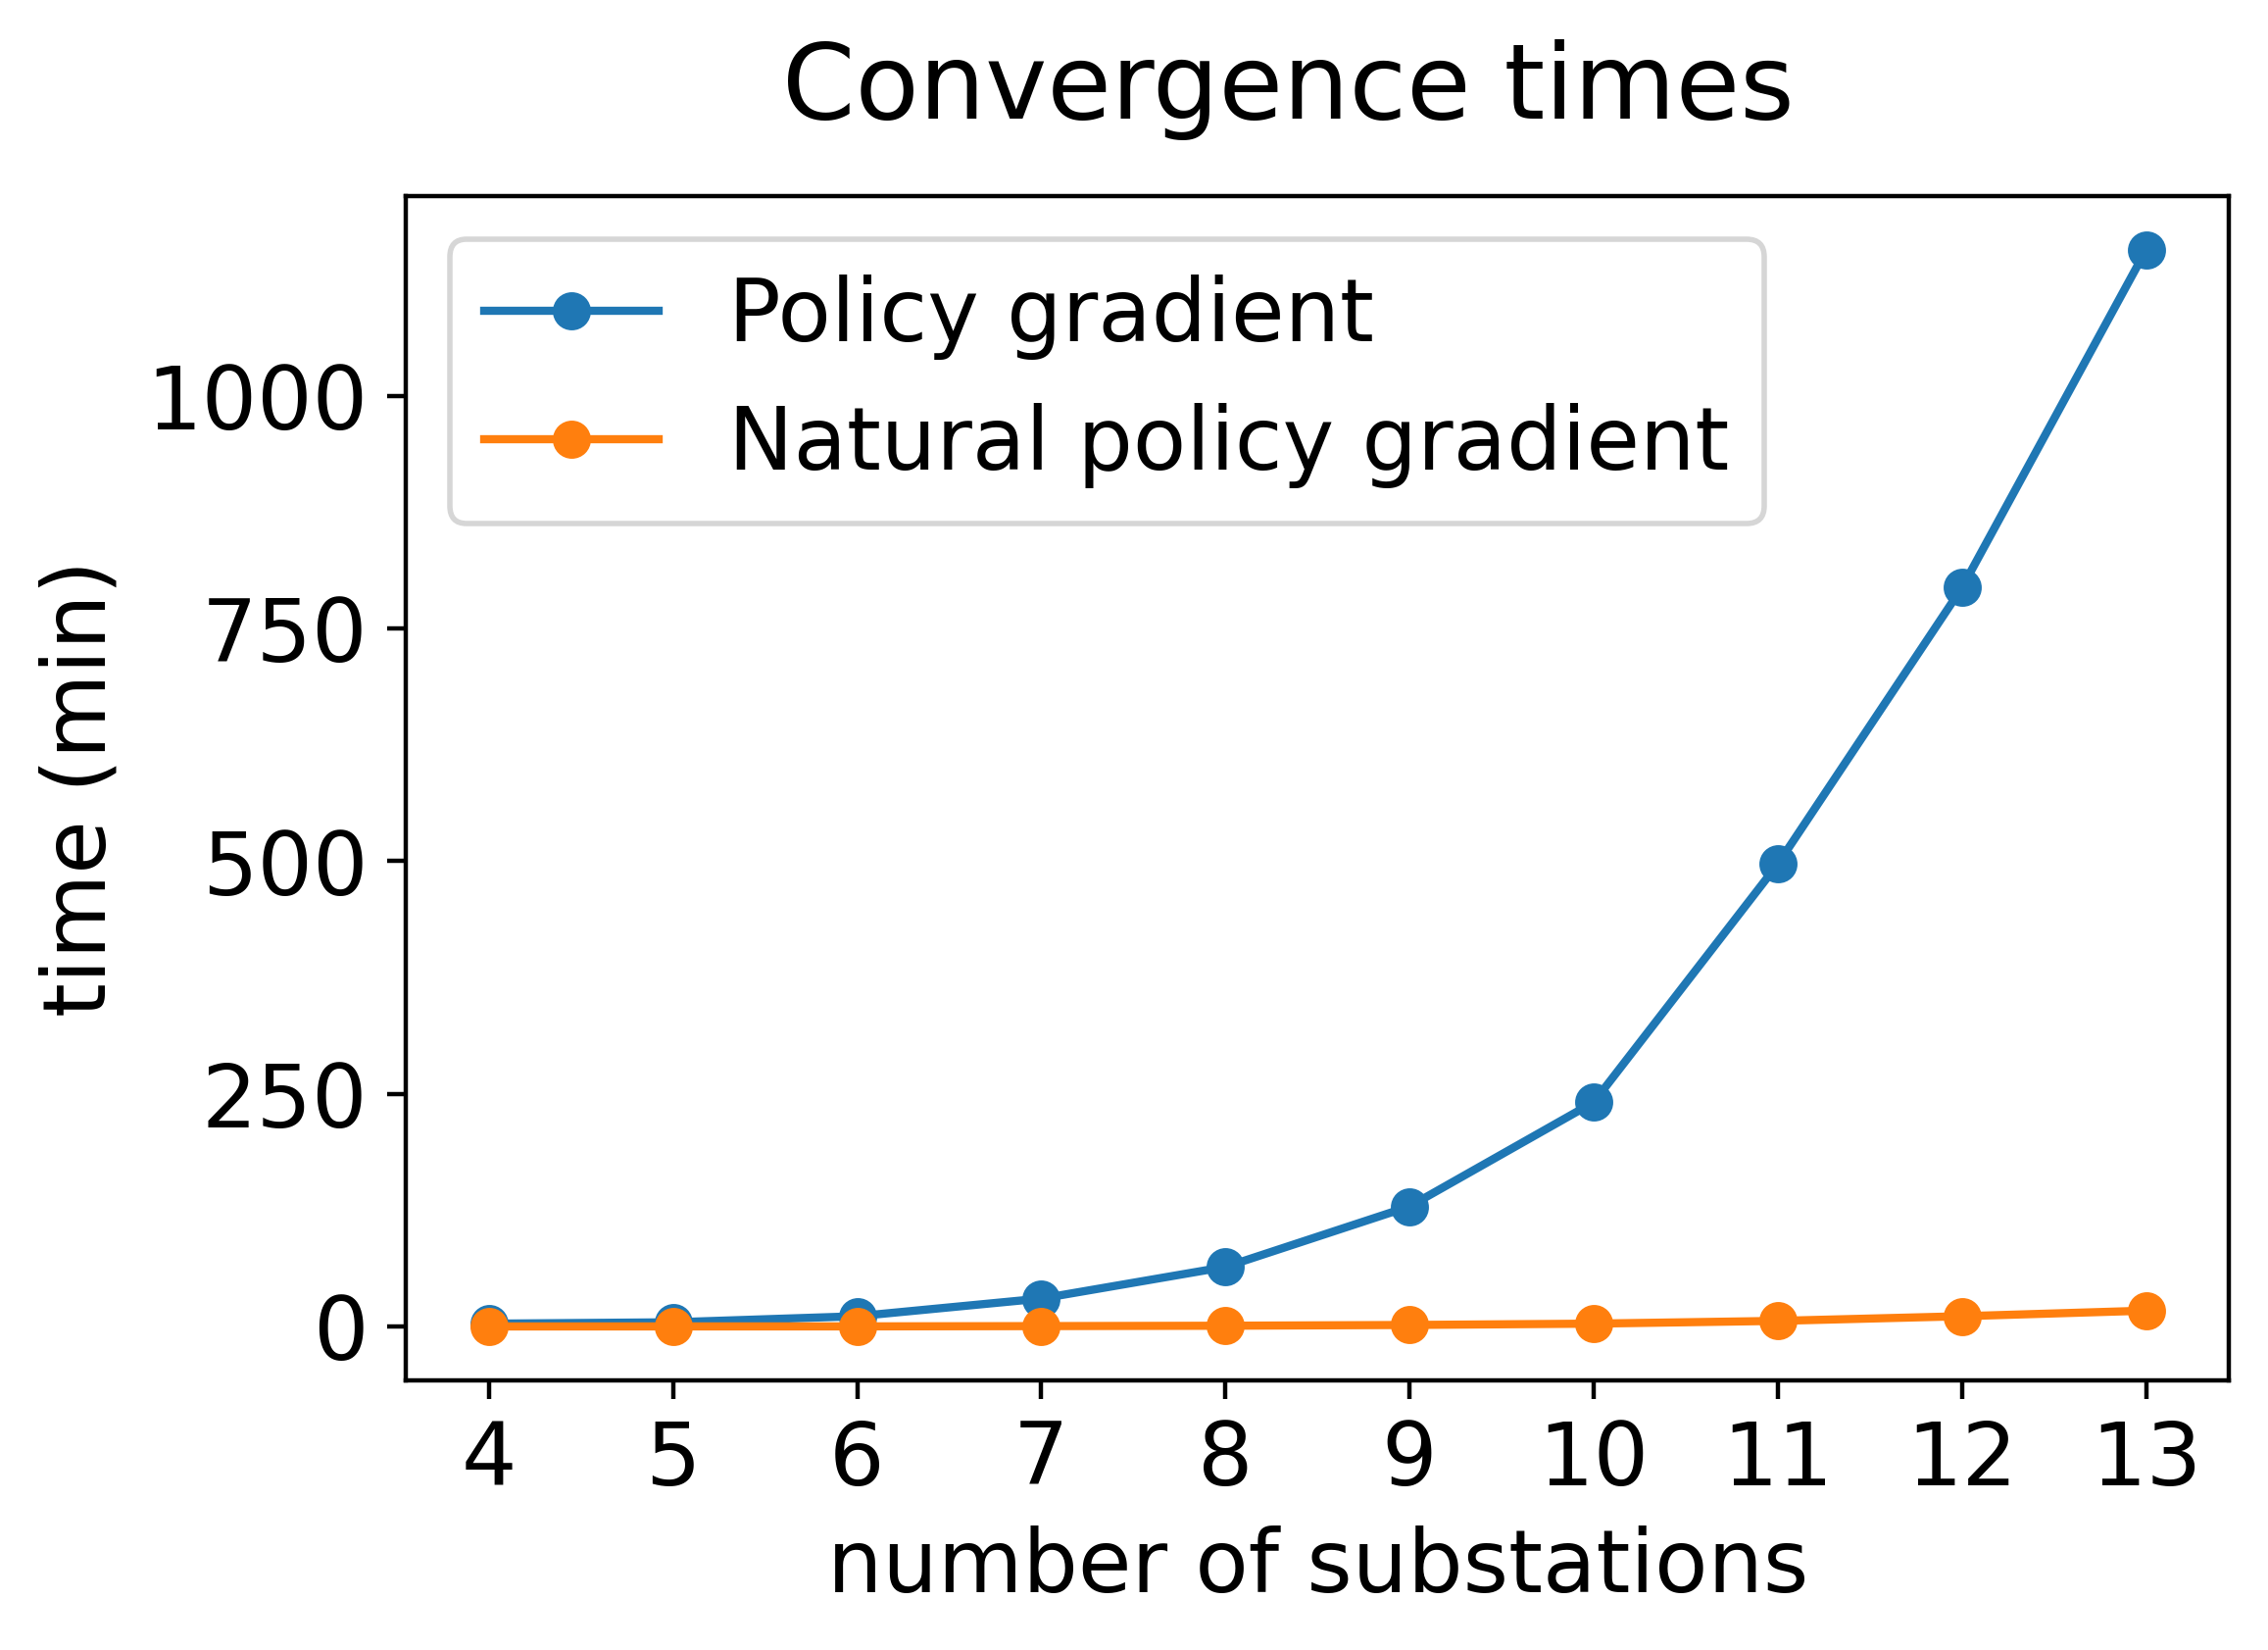
\includegraphics[scale=0.5]{figures/times_graph.png}
            \hspace*{-5pt}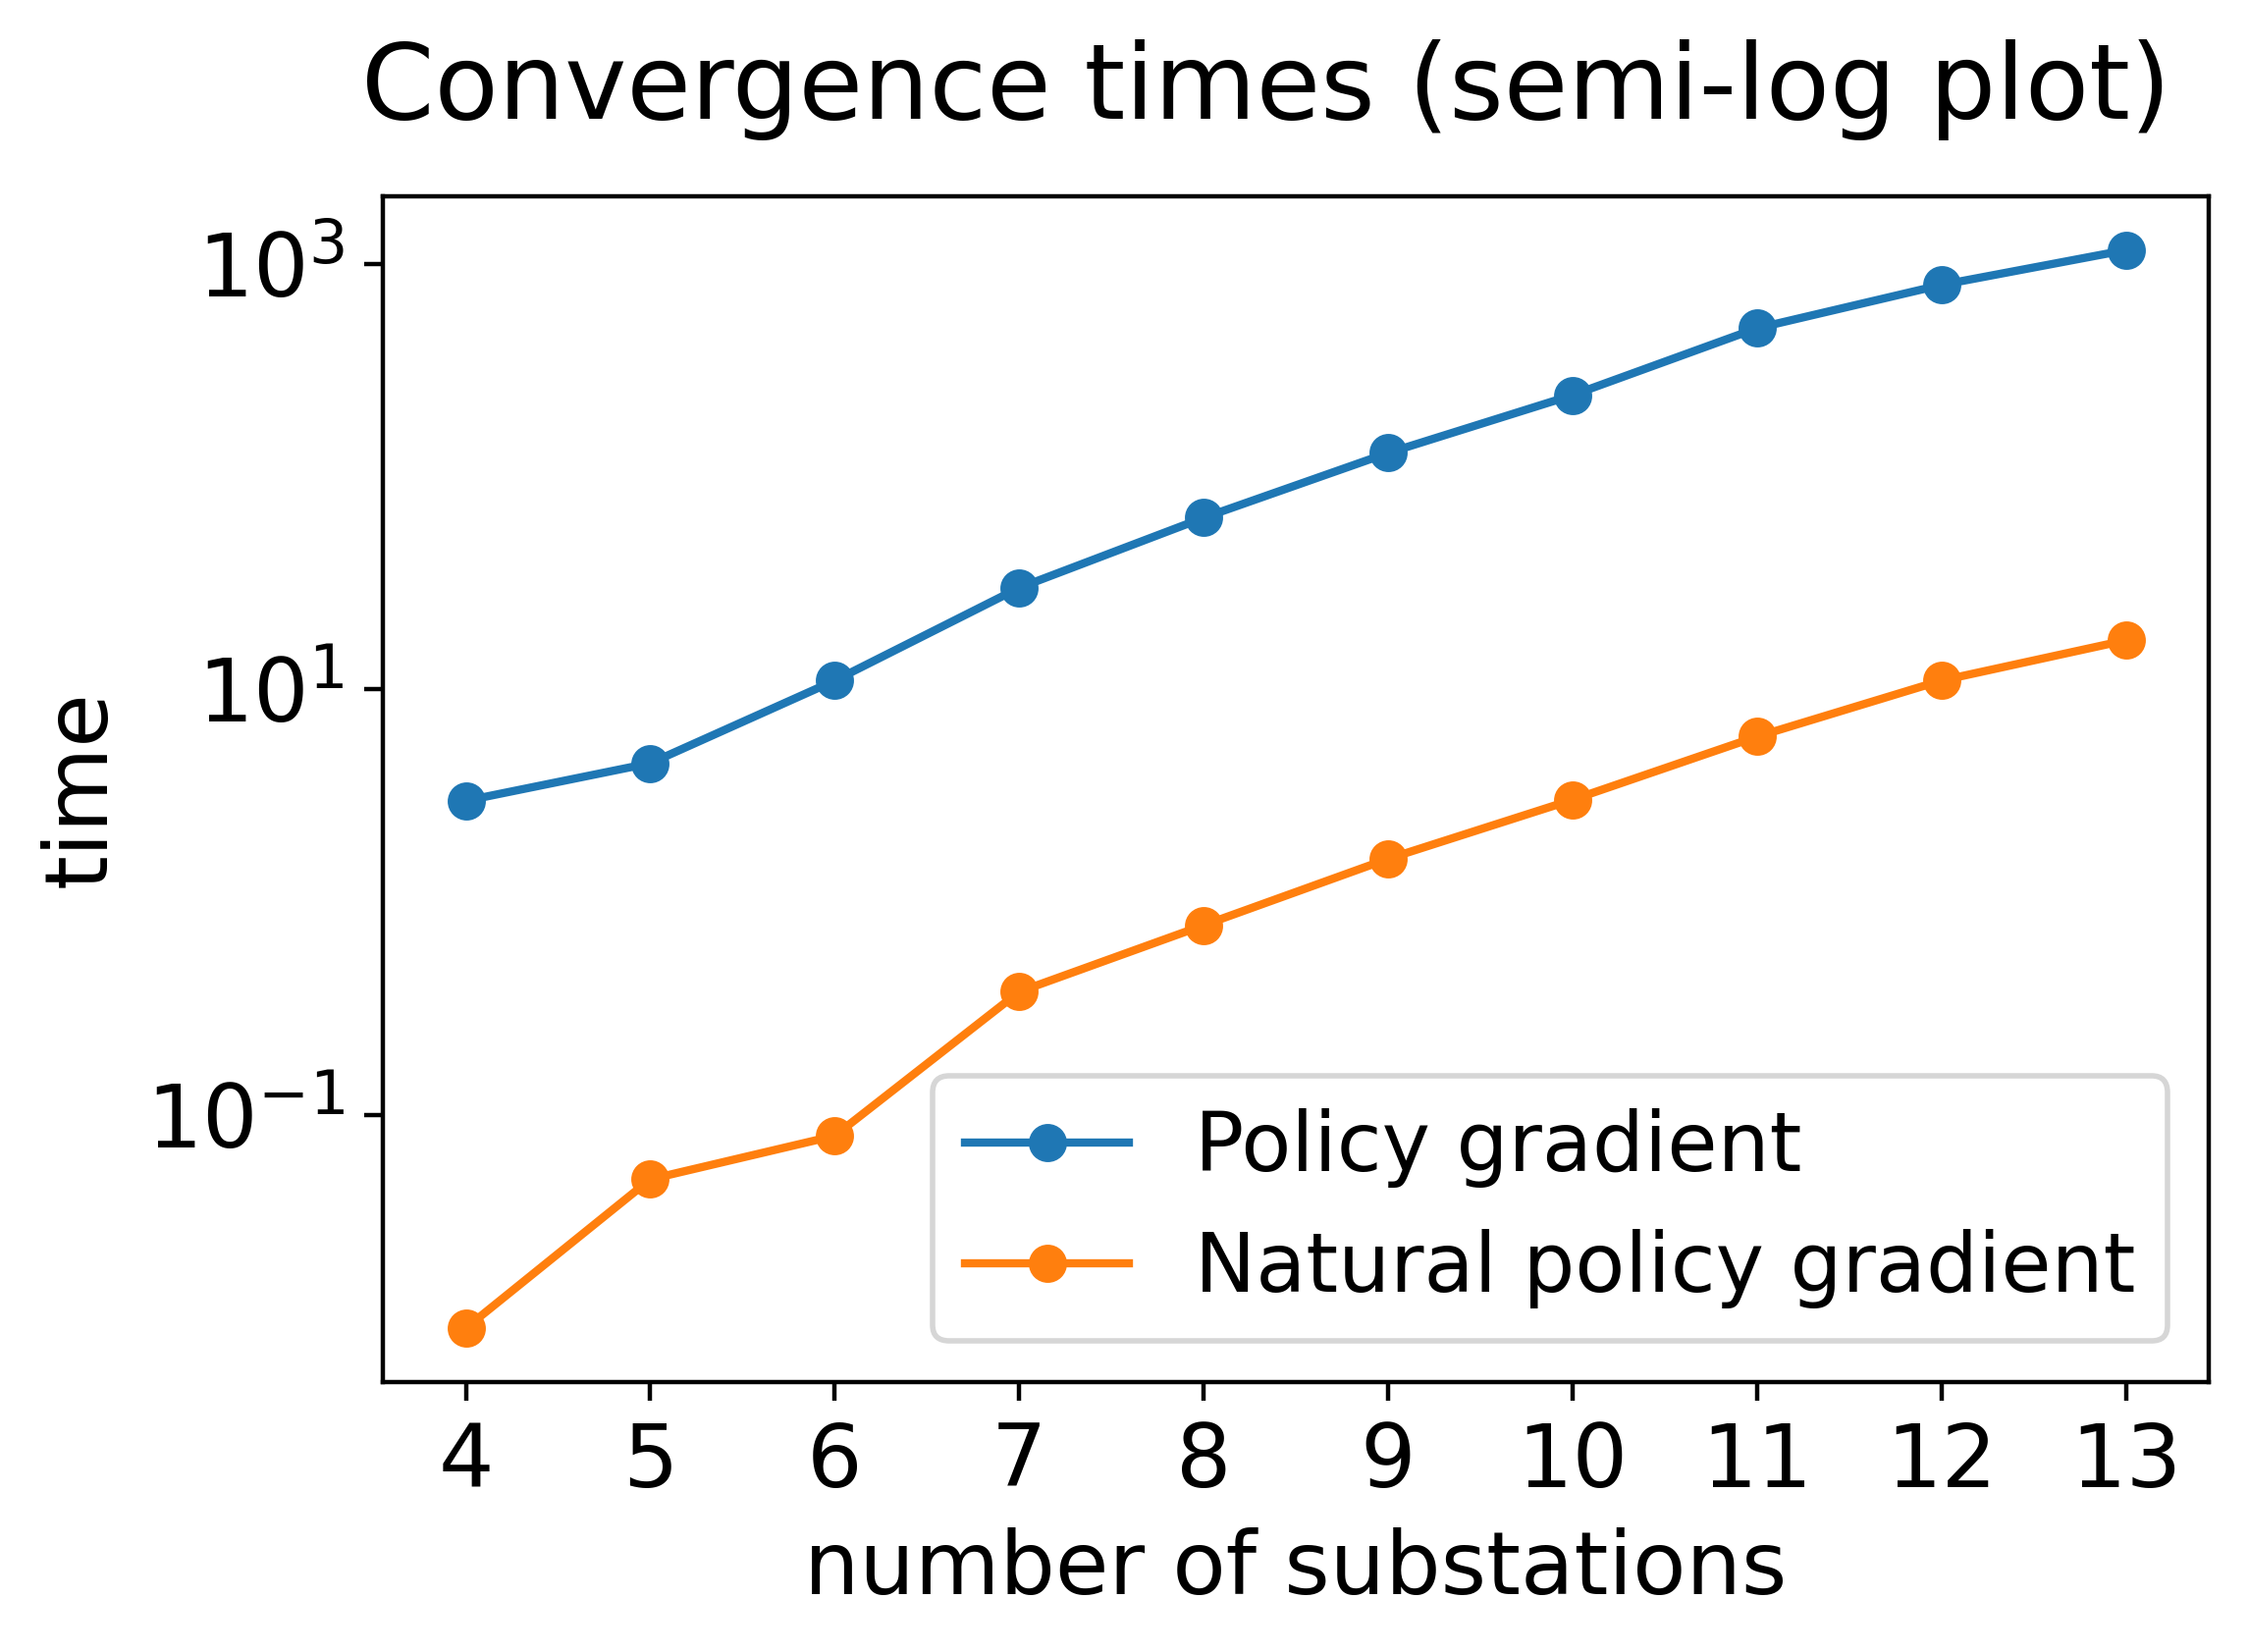
\includegraphics[scale=0.5]{figures/times_graph_log.png}
        }
    \end{figure}
    
\end{frame}

\begin{frame}{PG errors vs. NPG errors}

    \begin{figure}
        \centering
        \mbox{
            \hspace*{-10pt}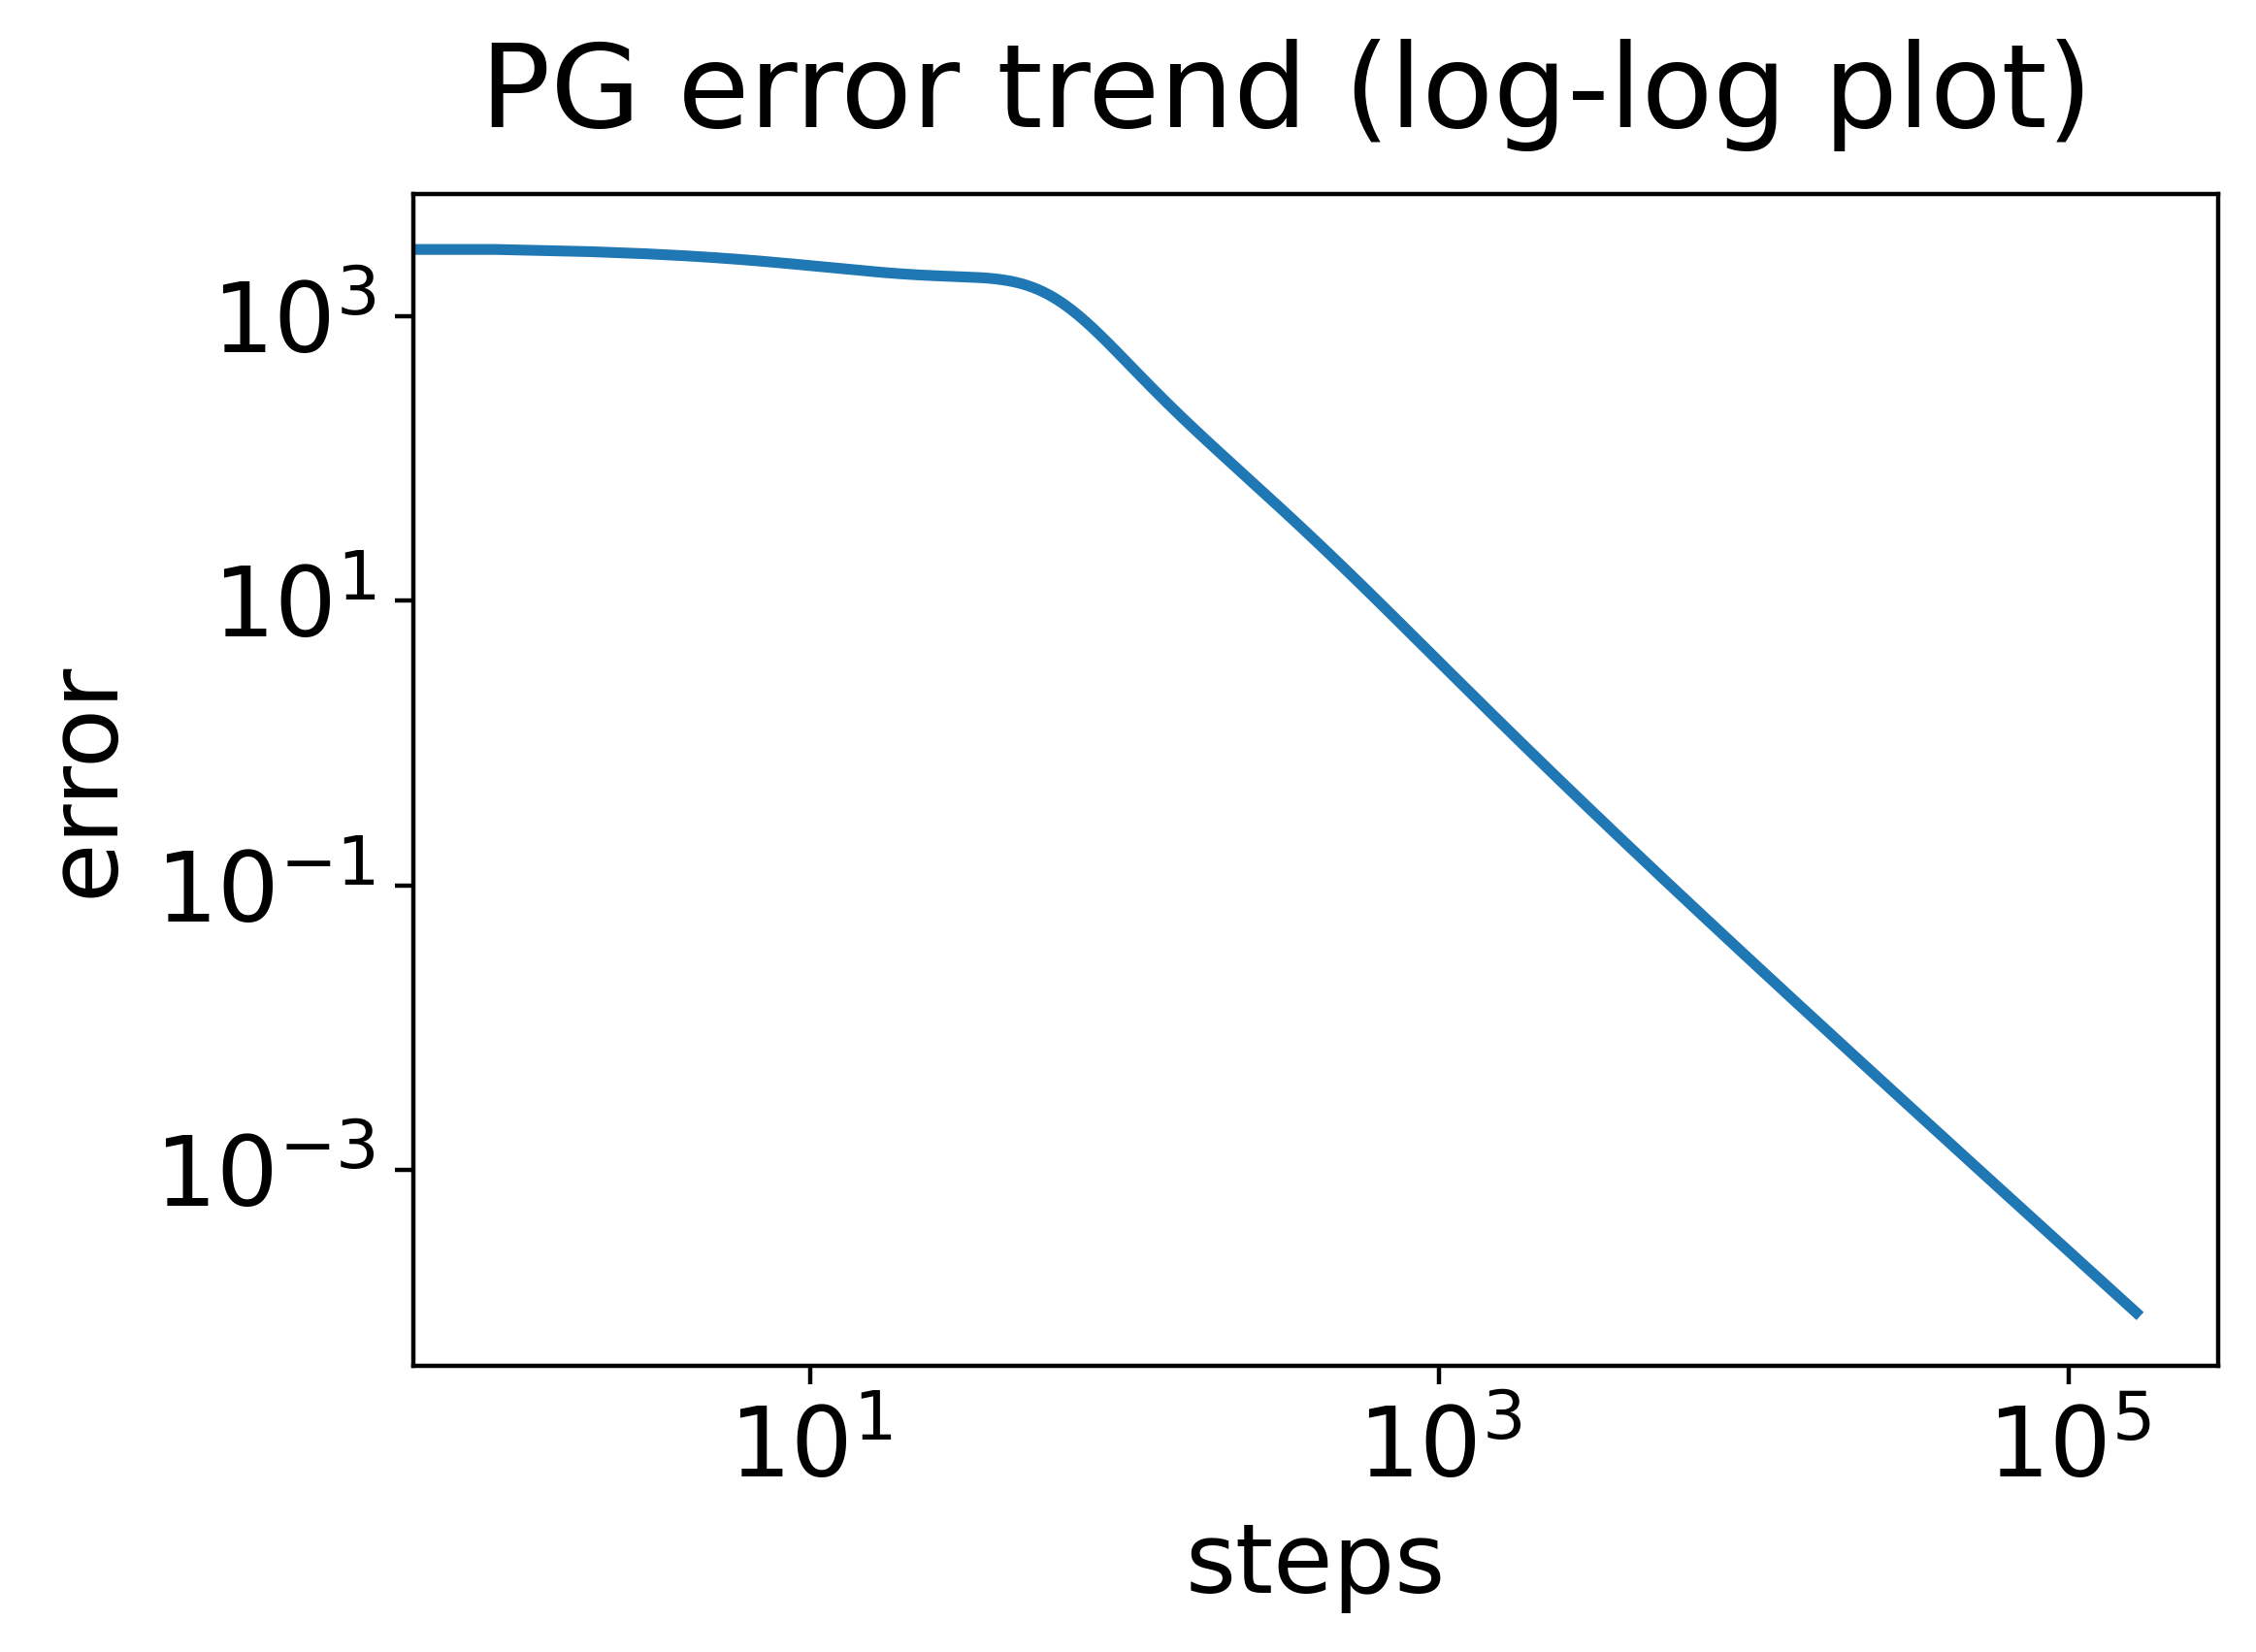
\includegraphics[scale=0.5]{figures/errors_log_log_PG.png}
            \hspace*{-5pt}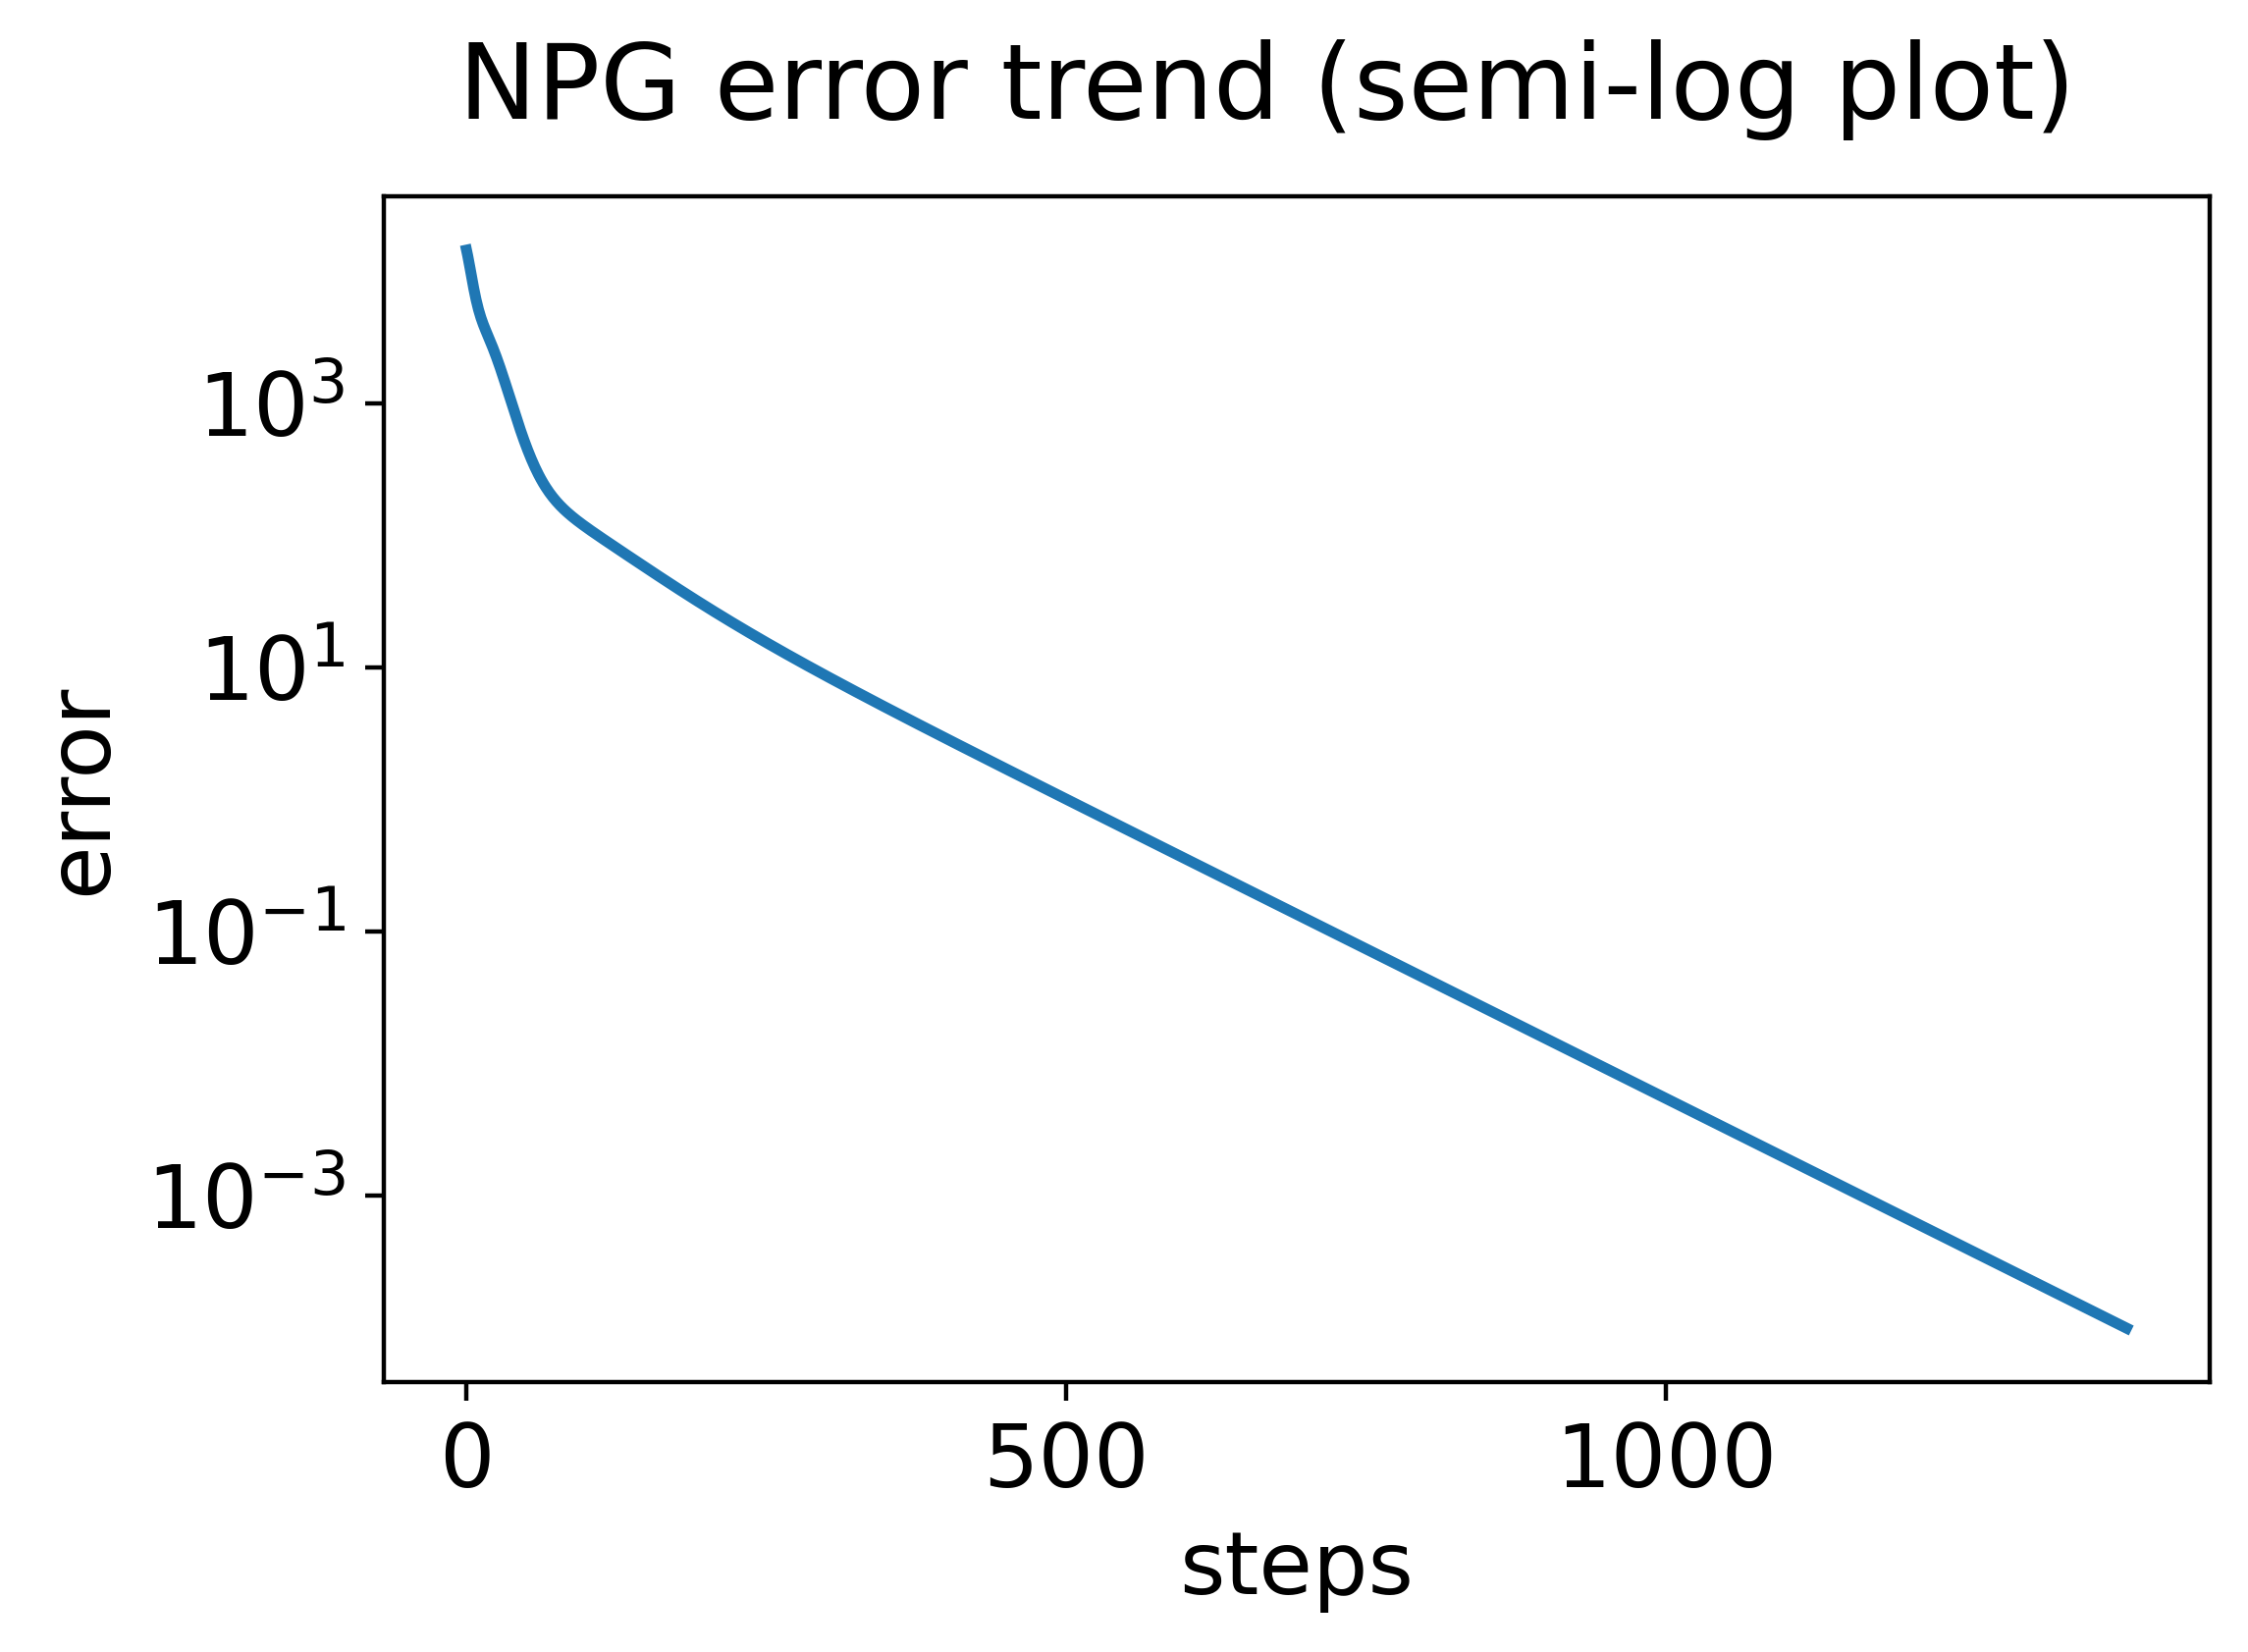
\includegraphics[scale=0.5]{figures/errors_log_NPG.png}
        }
    \end{figure}
    
\end{frame}

\begin{frame}{Trajectories of the parameters $\boldsymbol \theta$ for PG}
    
    \begin{figure}
        \centering
        \begin{tabular}{cc}
            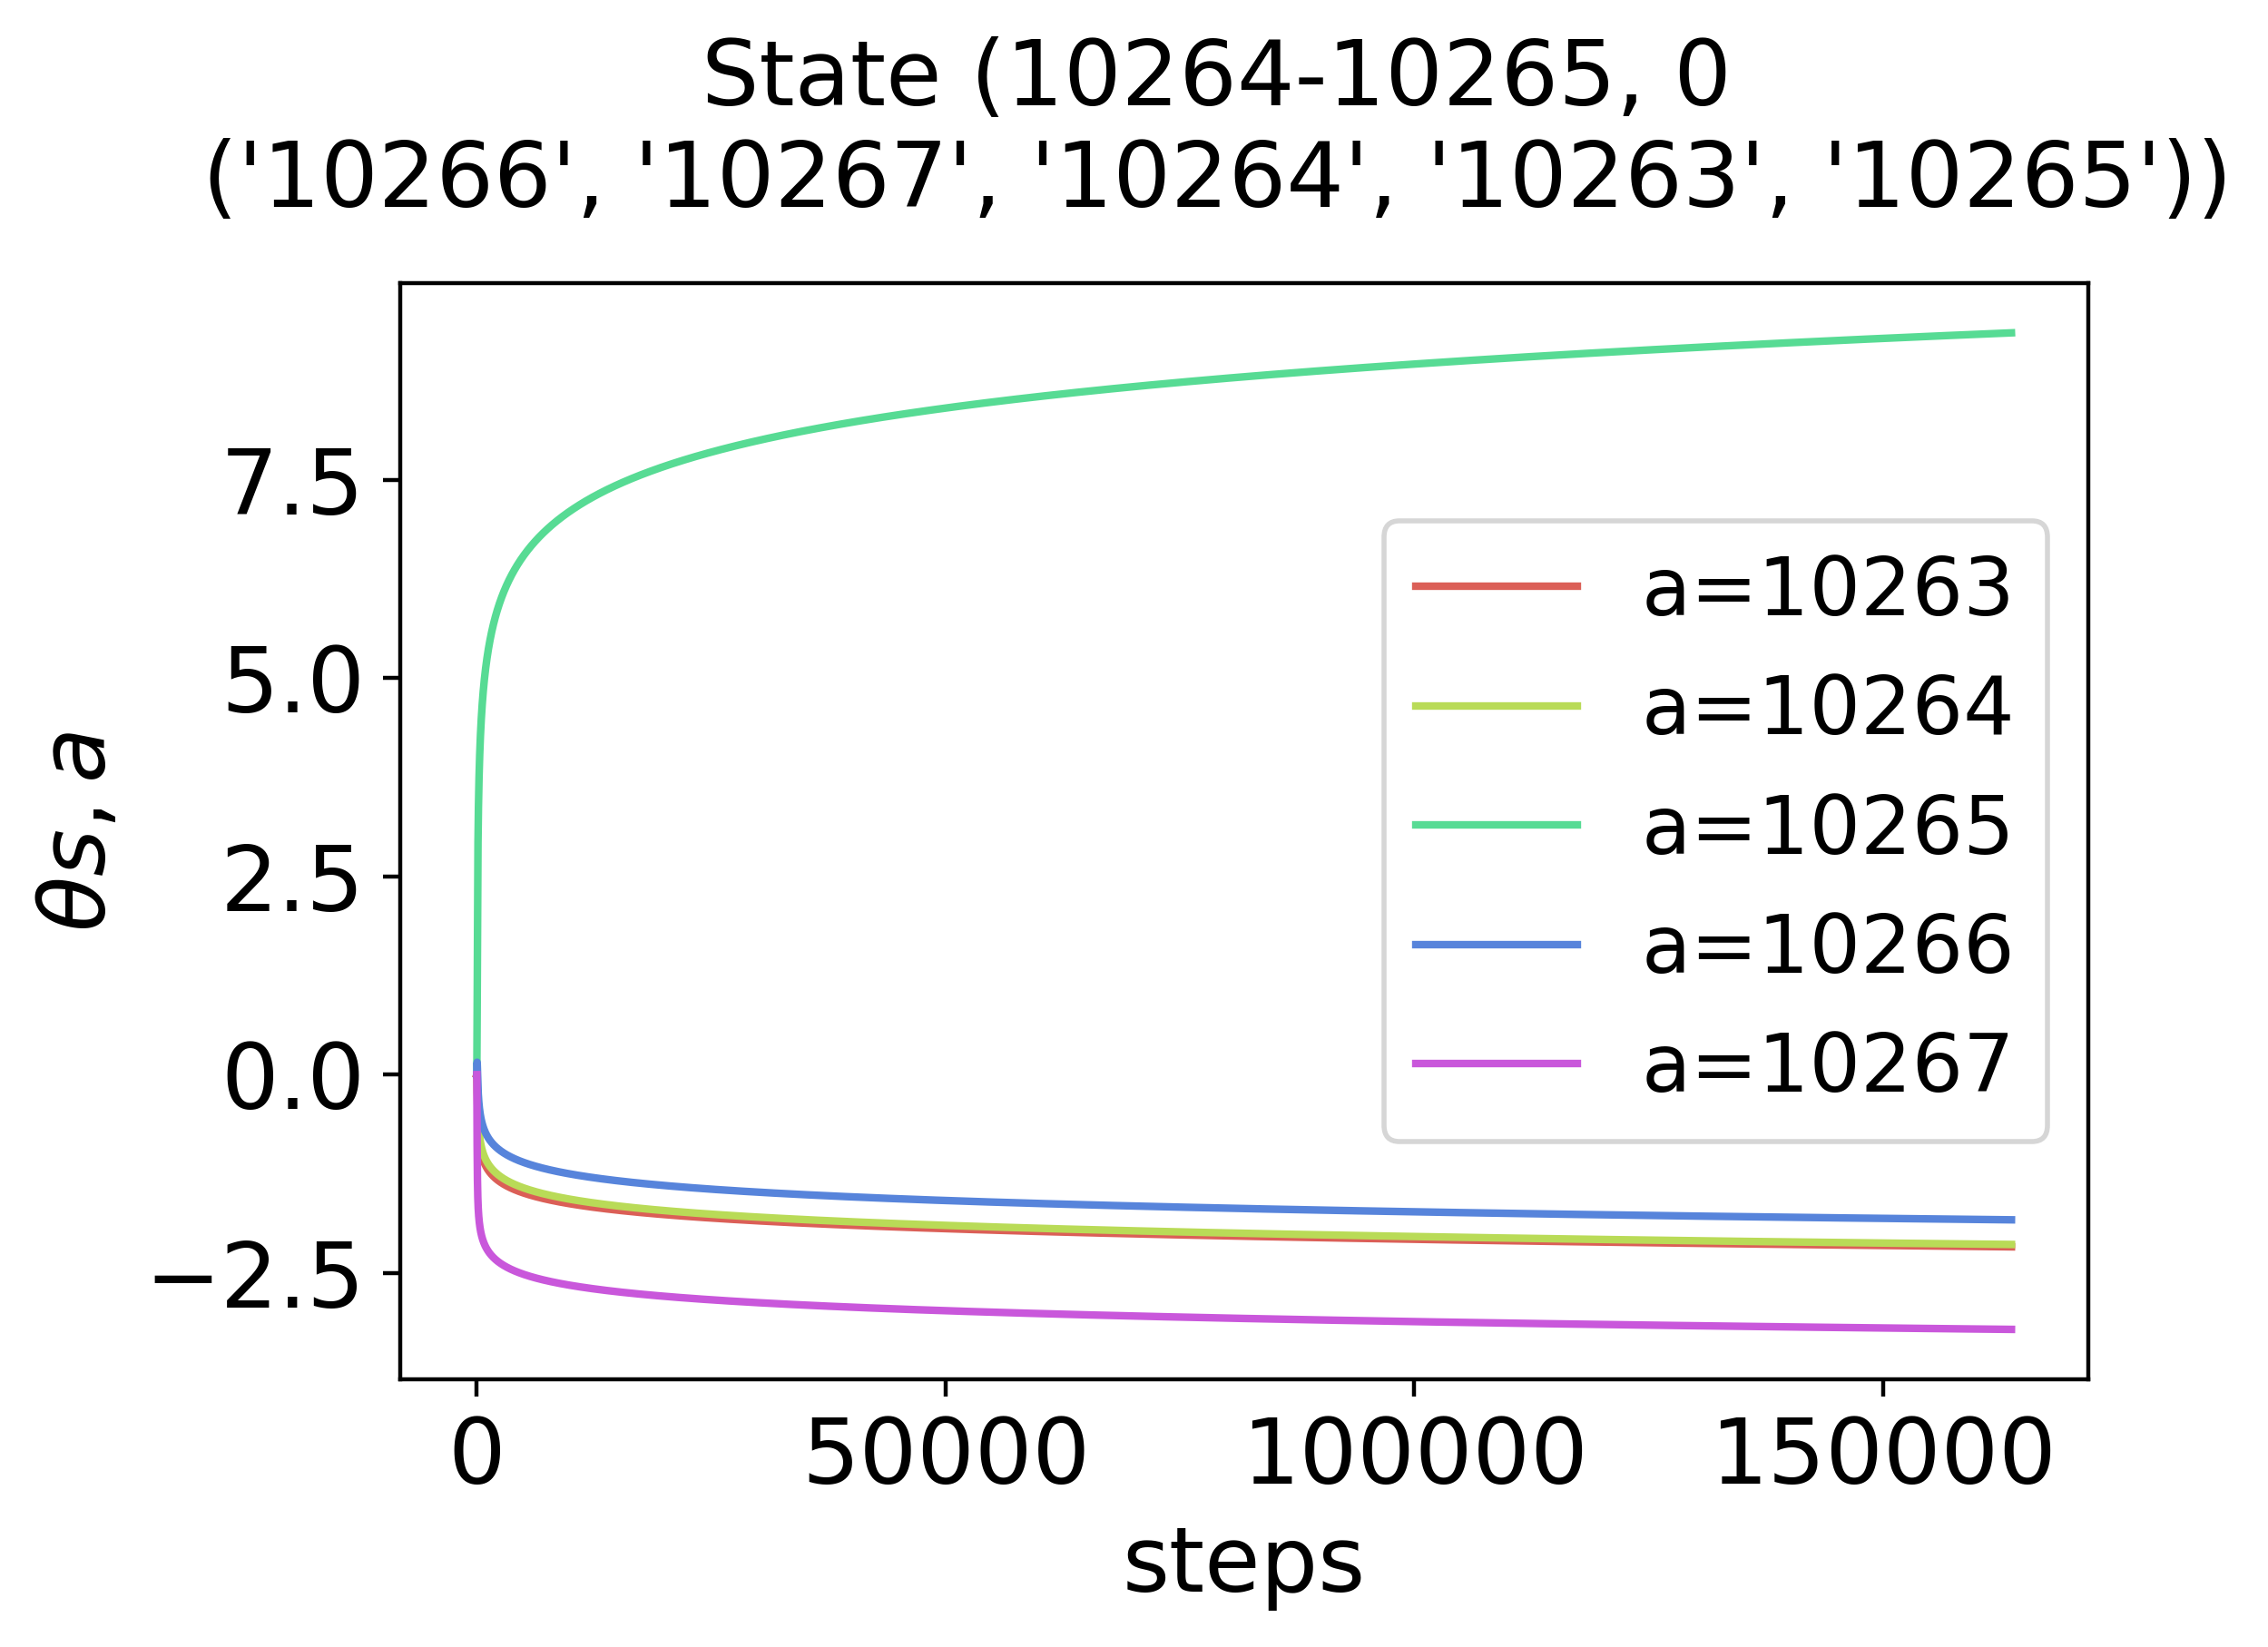
\includegraphics[scale=0.34,valign=b]{figures/theta_PG_state_0.png} &
            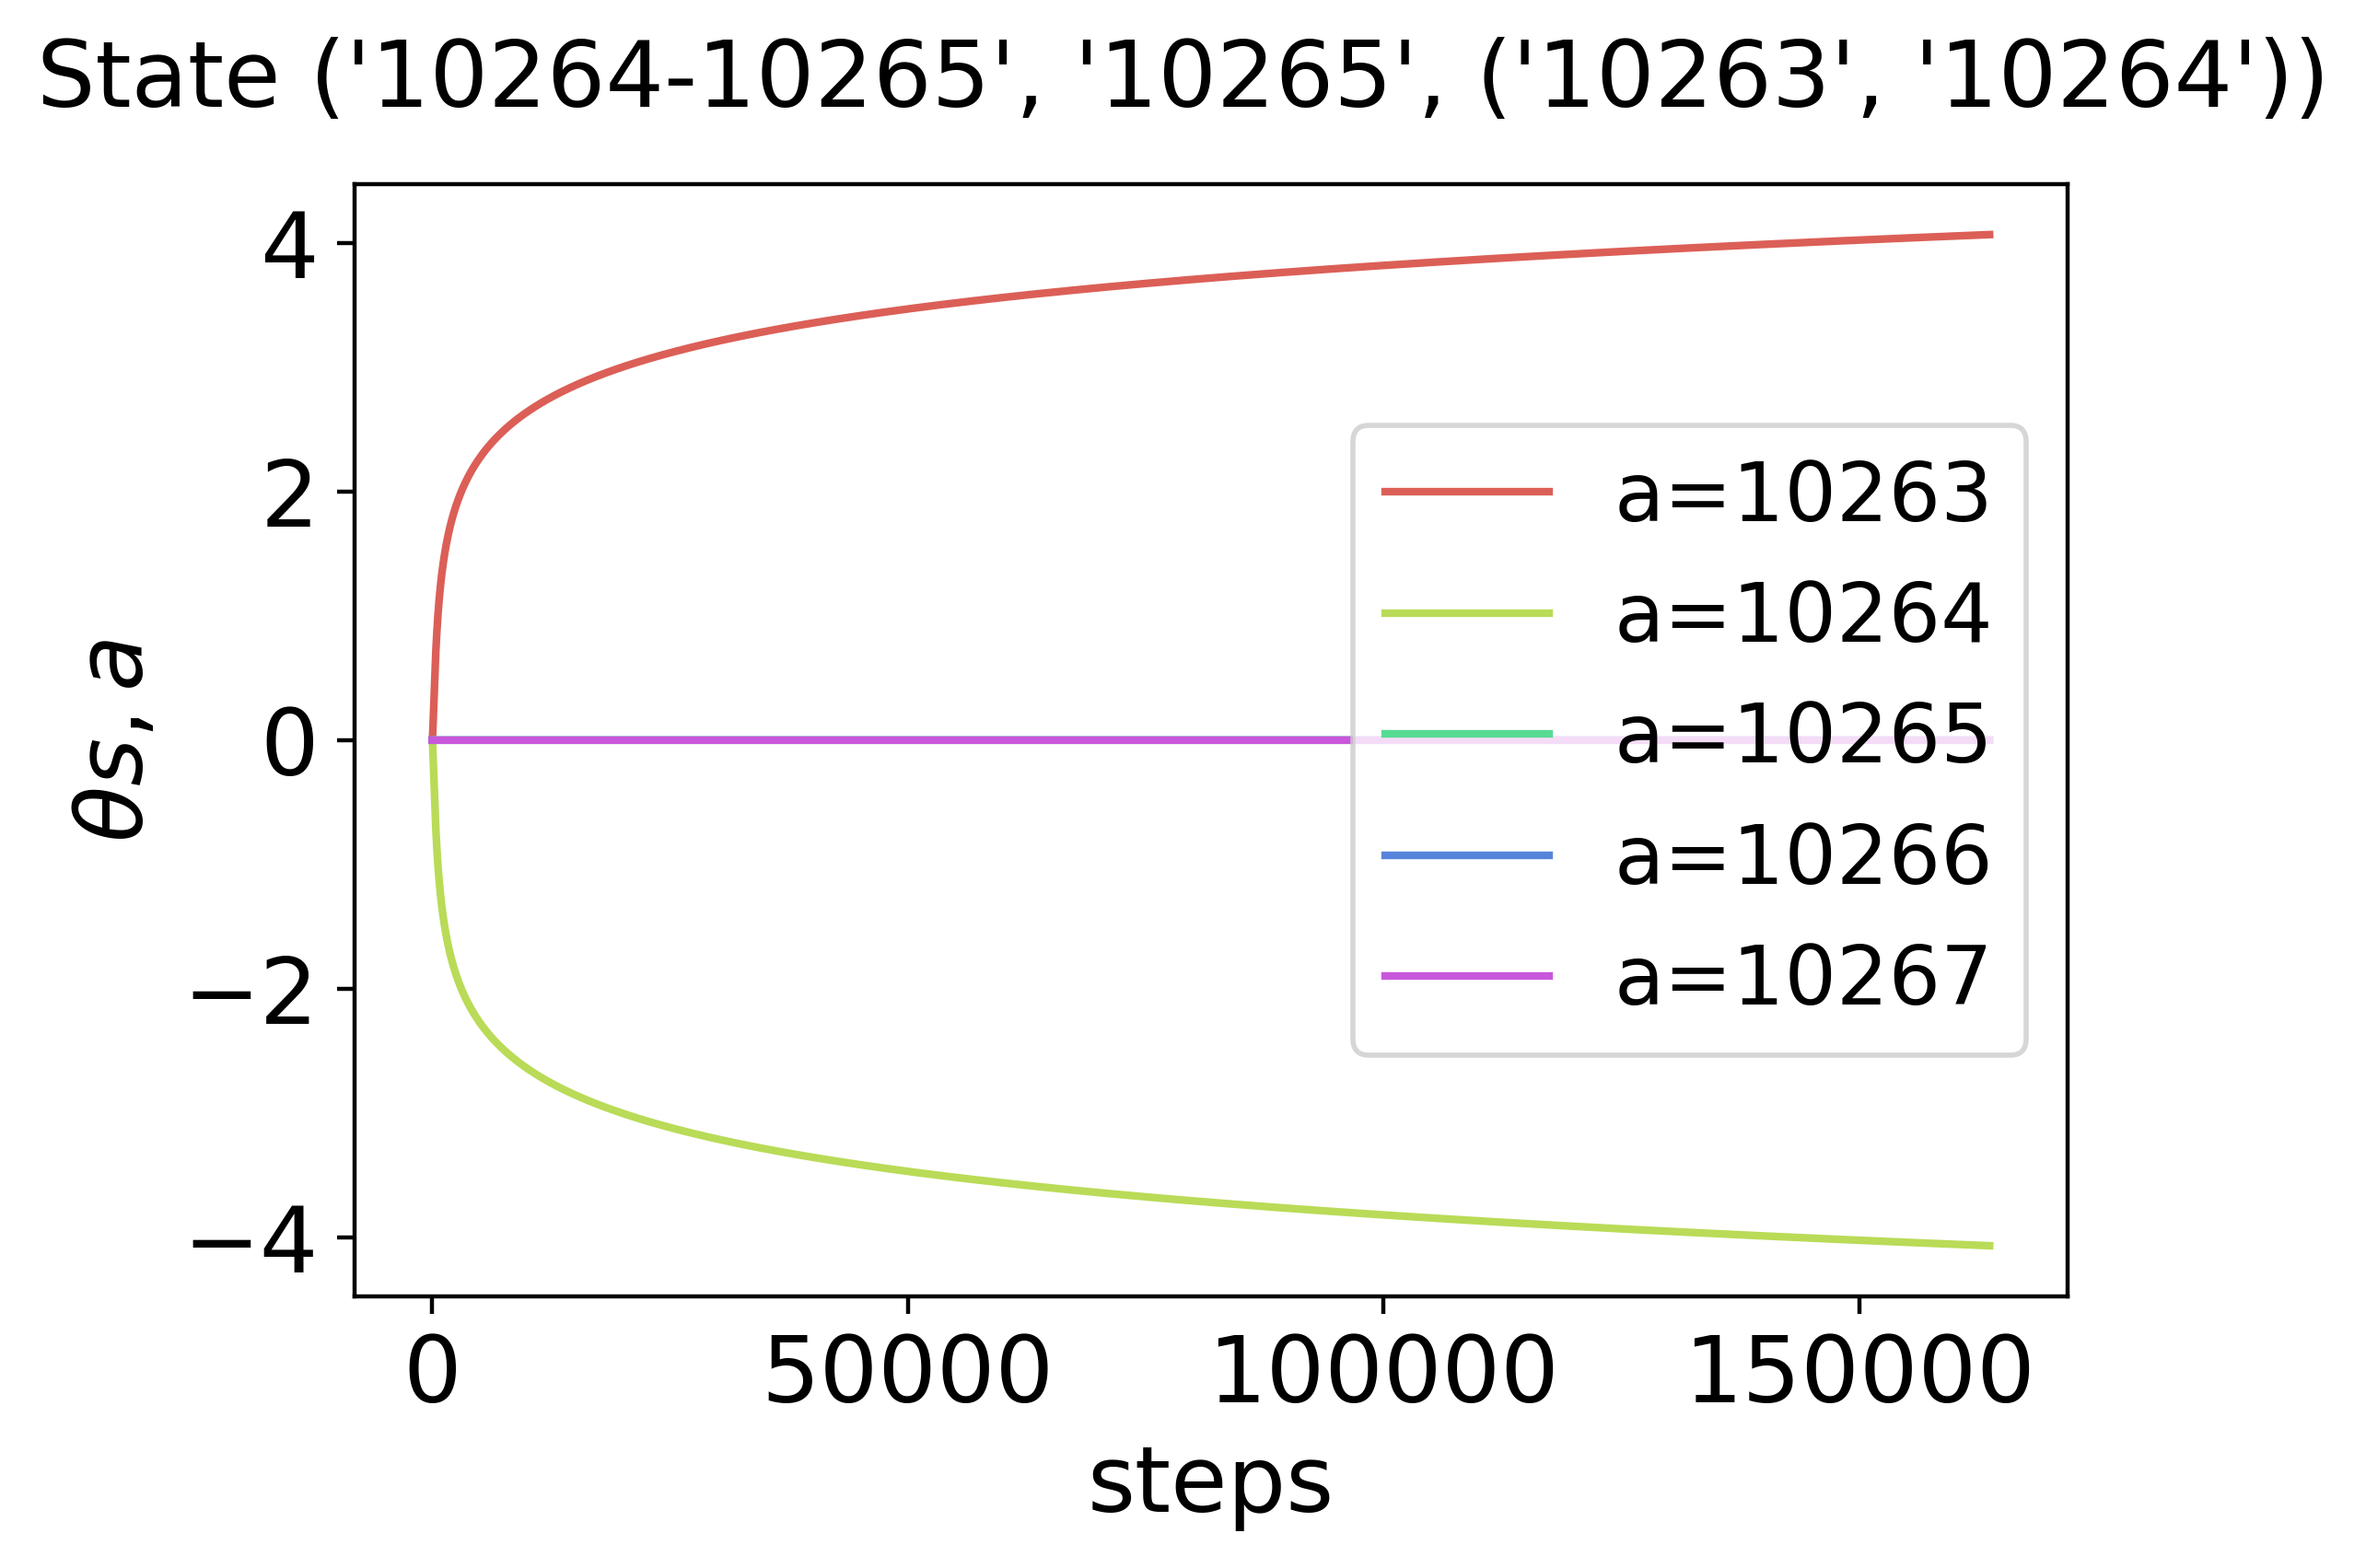
\includegraphics[scale=0.34,valign=b]{figures/theta_PG_state_1.png} \\
            \hspace*{-10pt}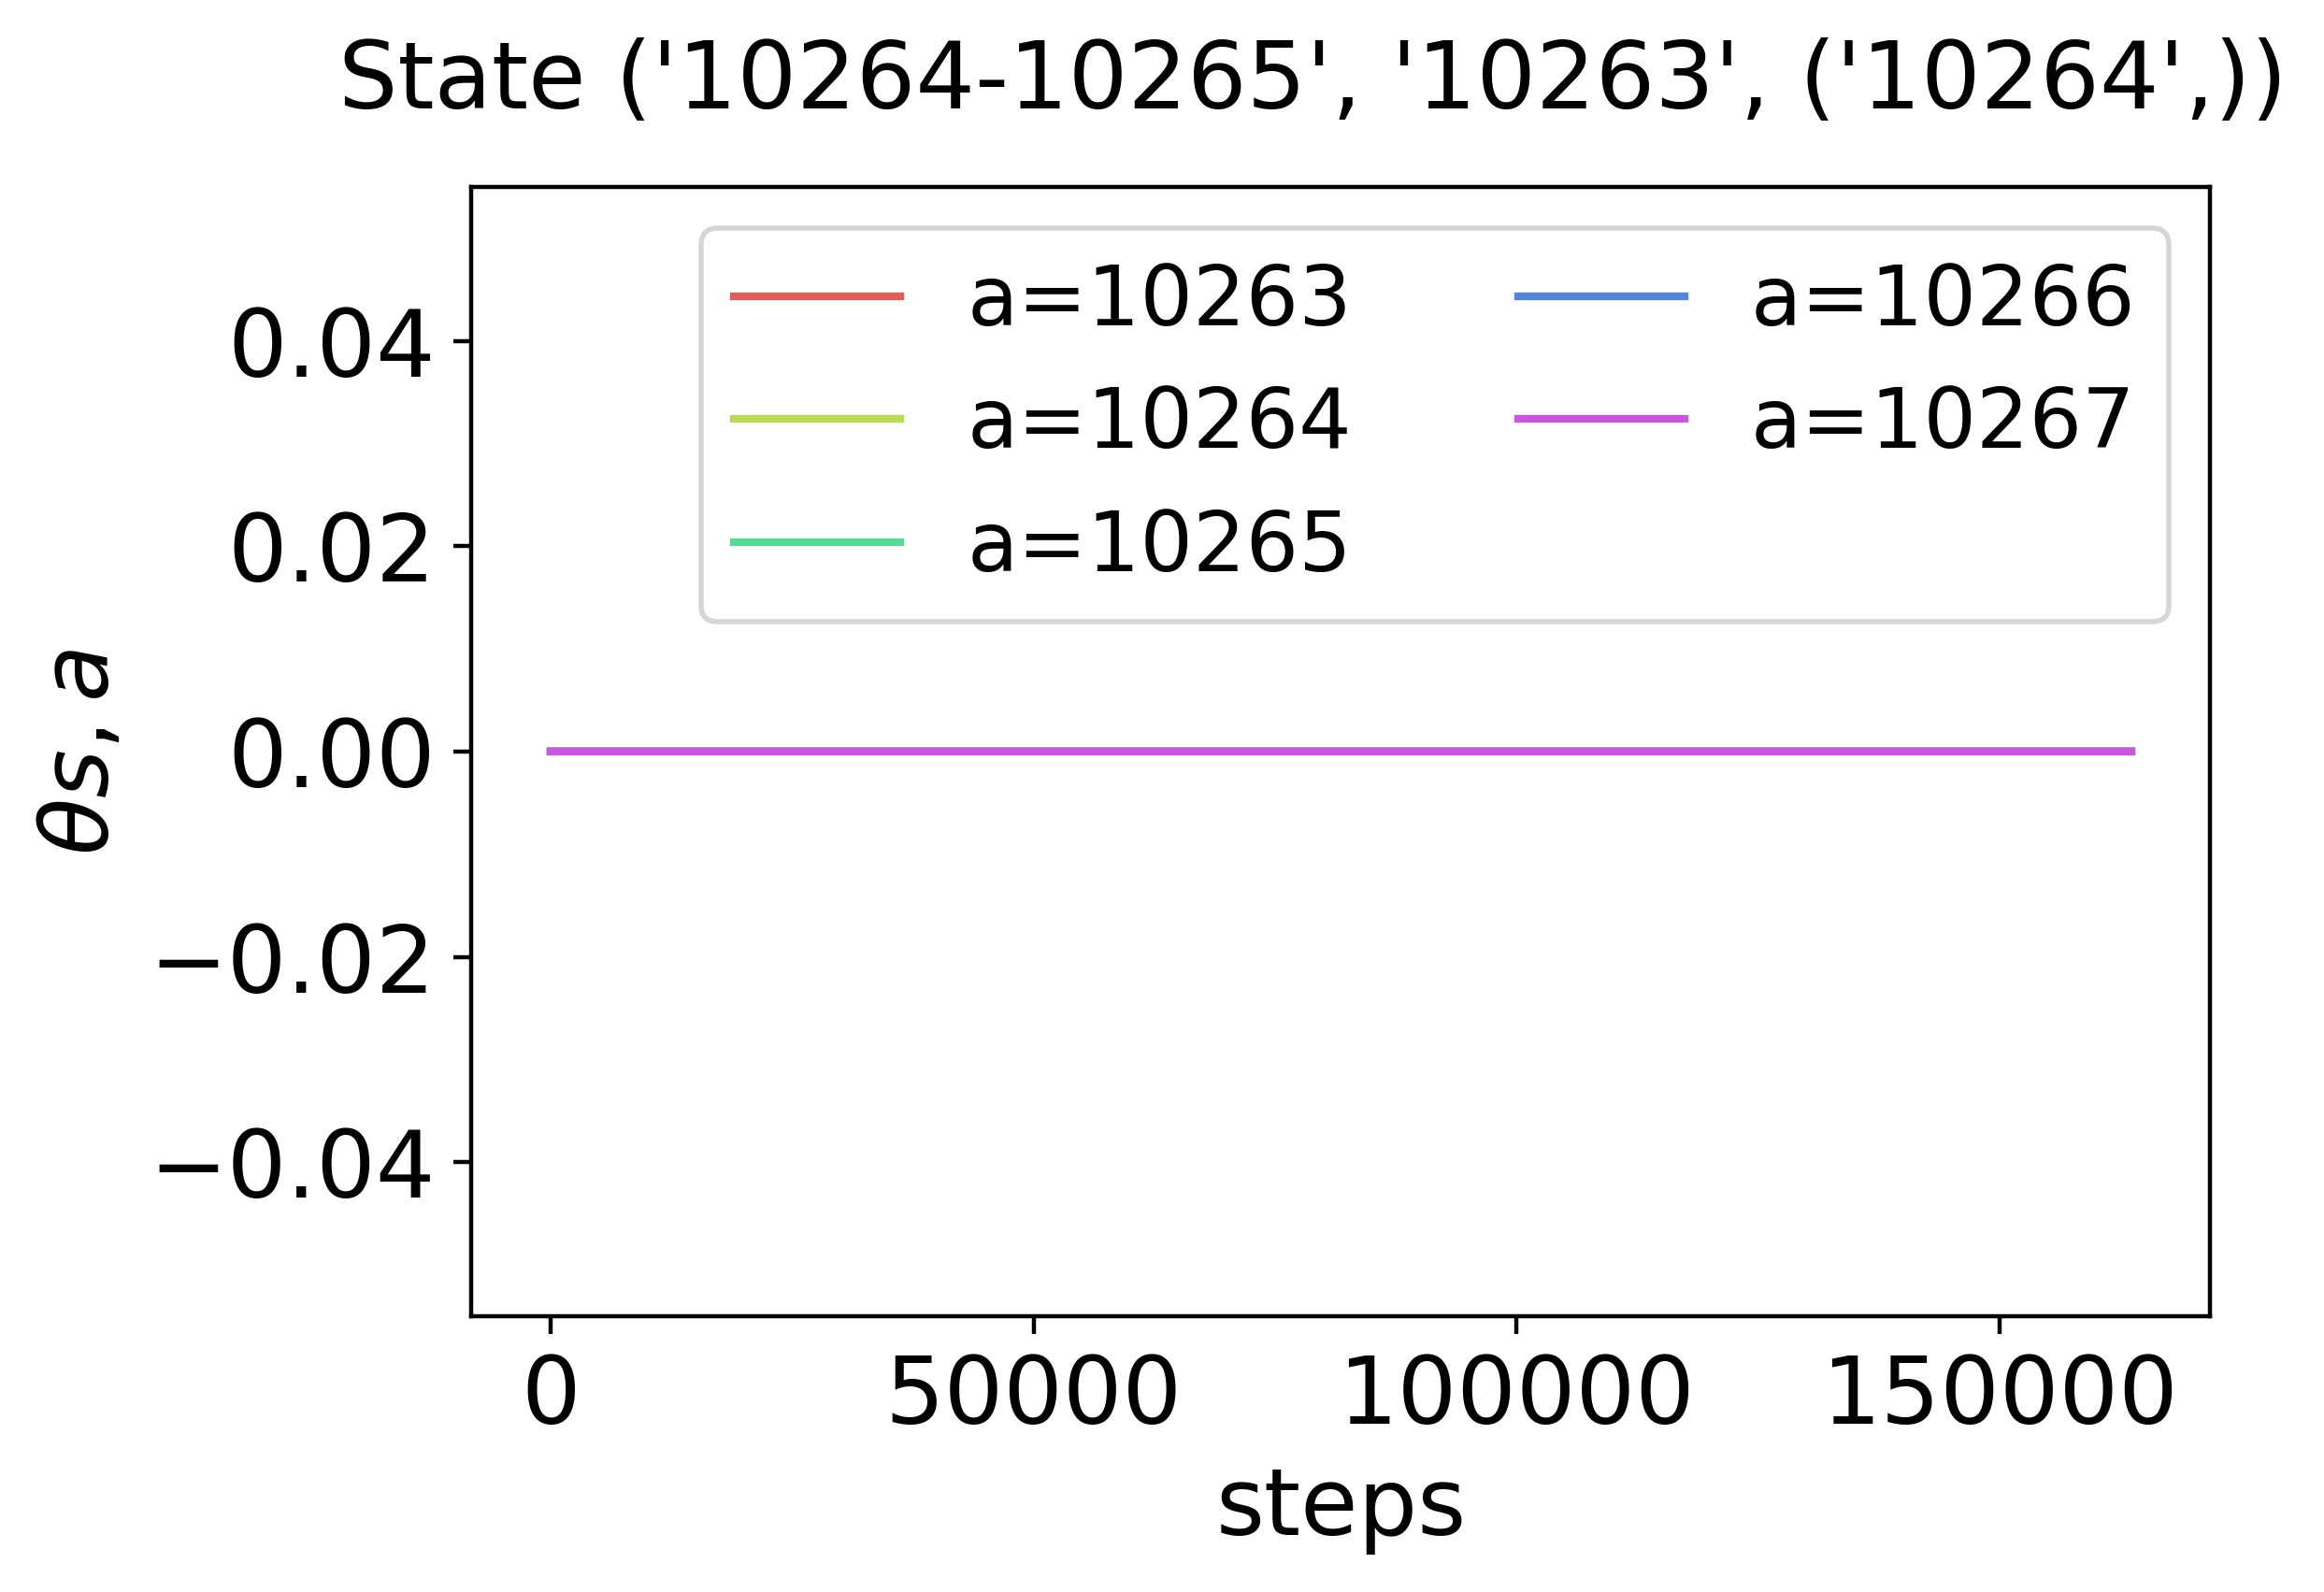
\includegraphics[scale=0.34,valign=b]{figures/theta_PG_state_2.png} &
            \hspace*{-28pt}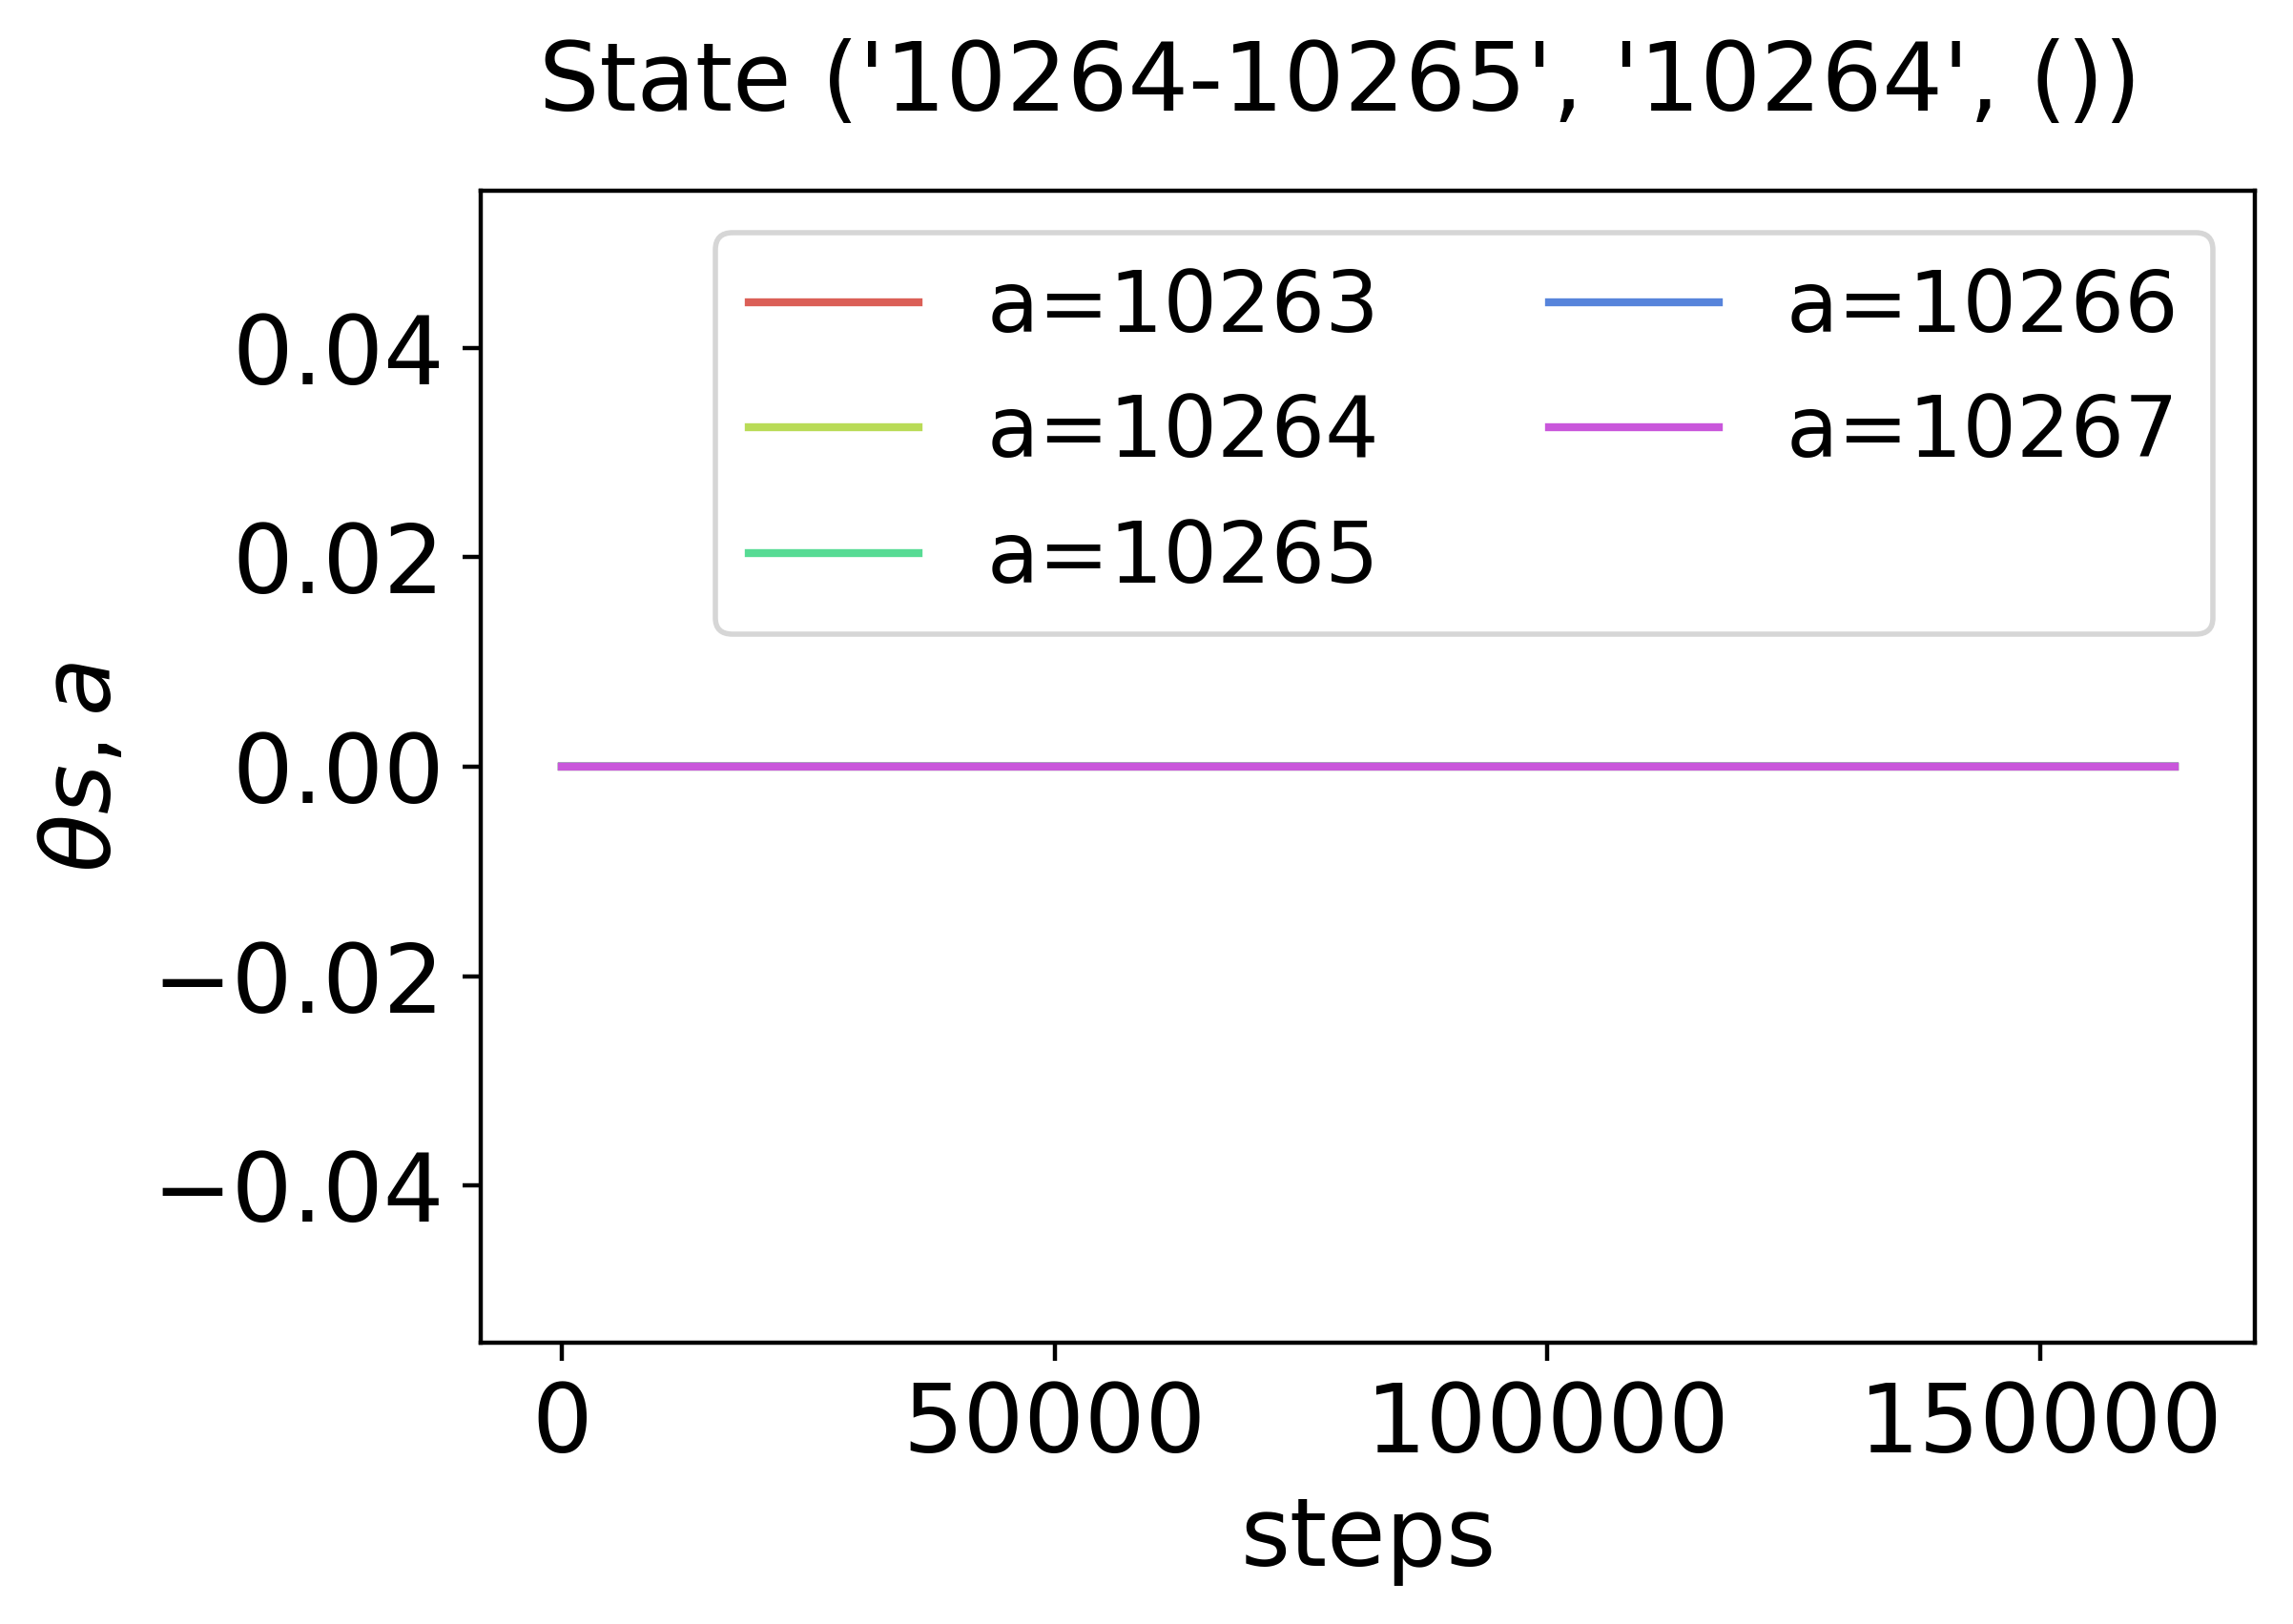
\includegraphics[scale=0.34,valign=b]{figures/theta_PG_state_3.png}
        \end{tabular}
    \end{figure}
\end{frame}

\begin{frame}{Trajectories of the policies $\pi_{\boldsymbol \theta}$ for PG}

    \begin{figure}
        \centering
        \begin{tabular}{cc}
            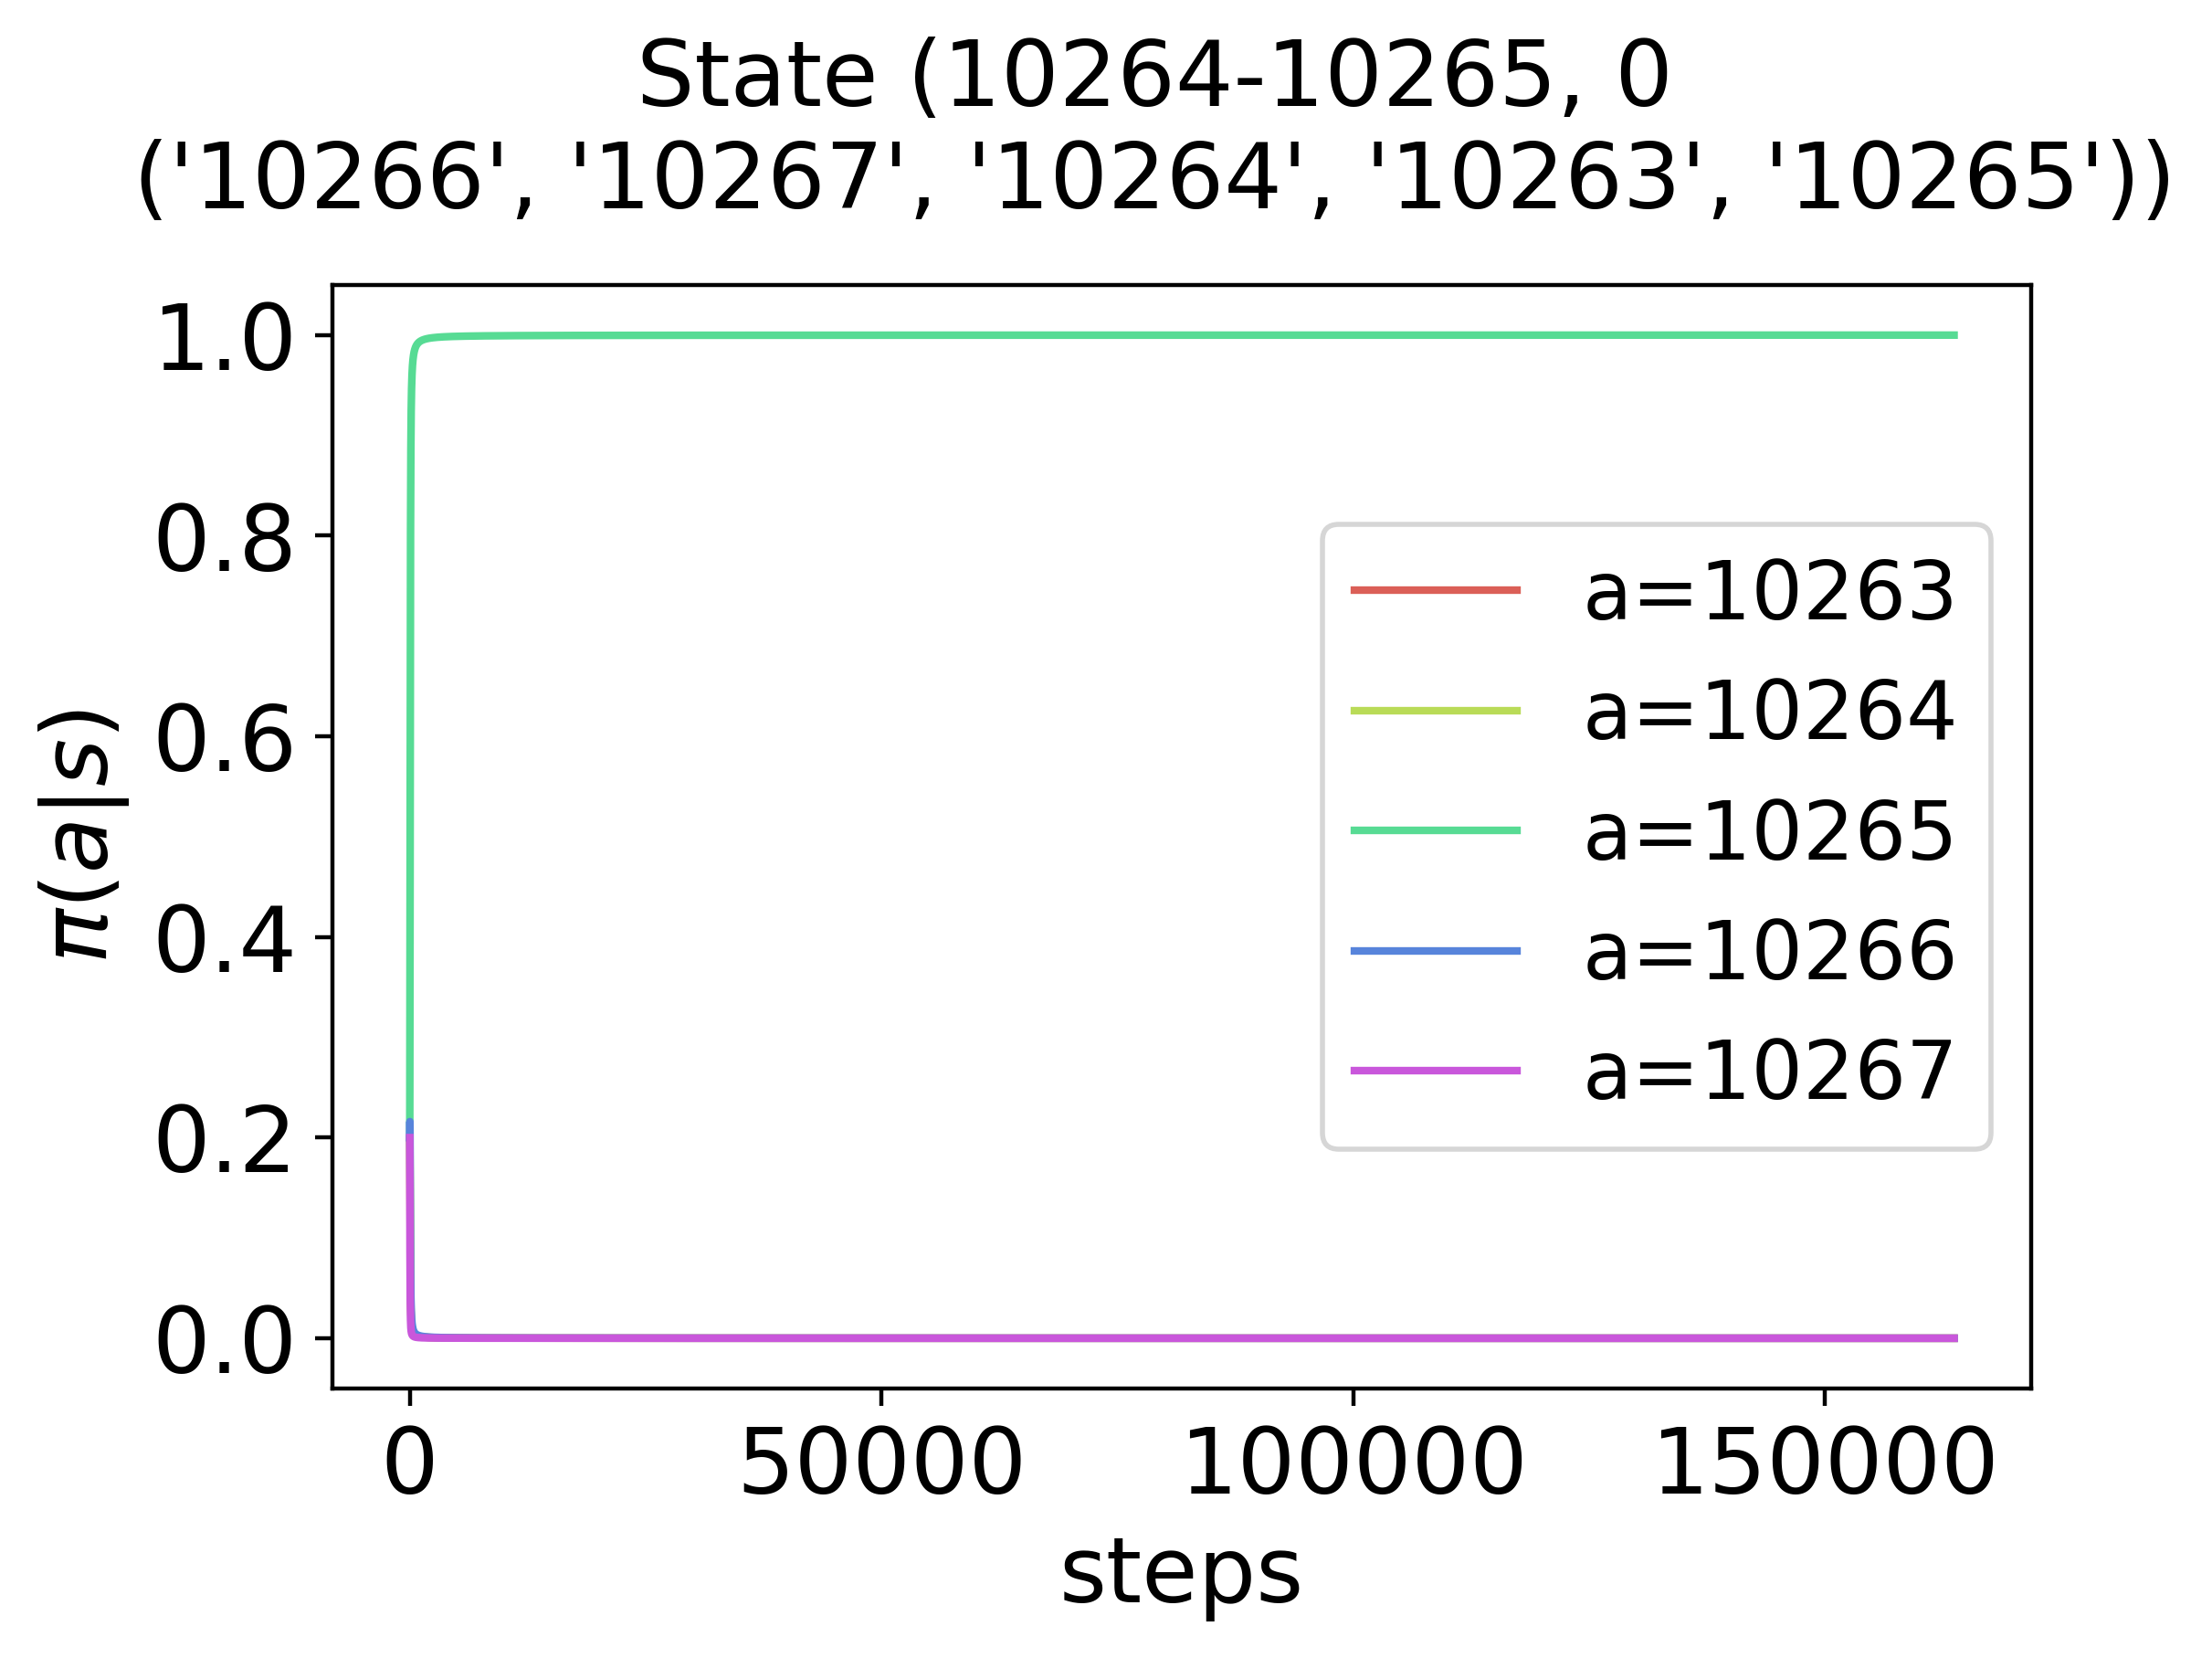
\includegraphics[scale=0.34,valign=b]{figures/policy_PG_state_0.png} &
            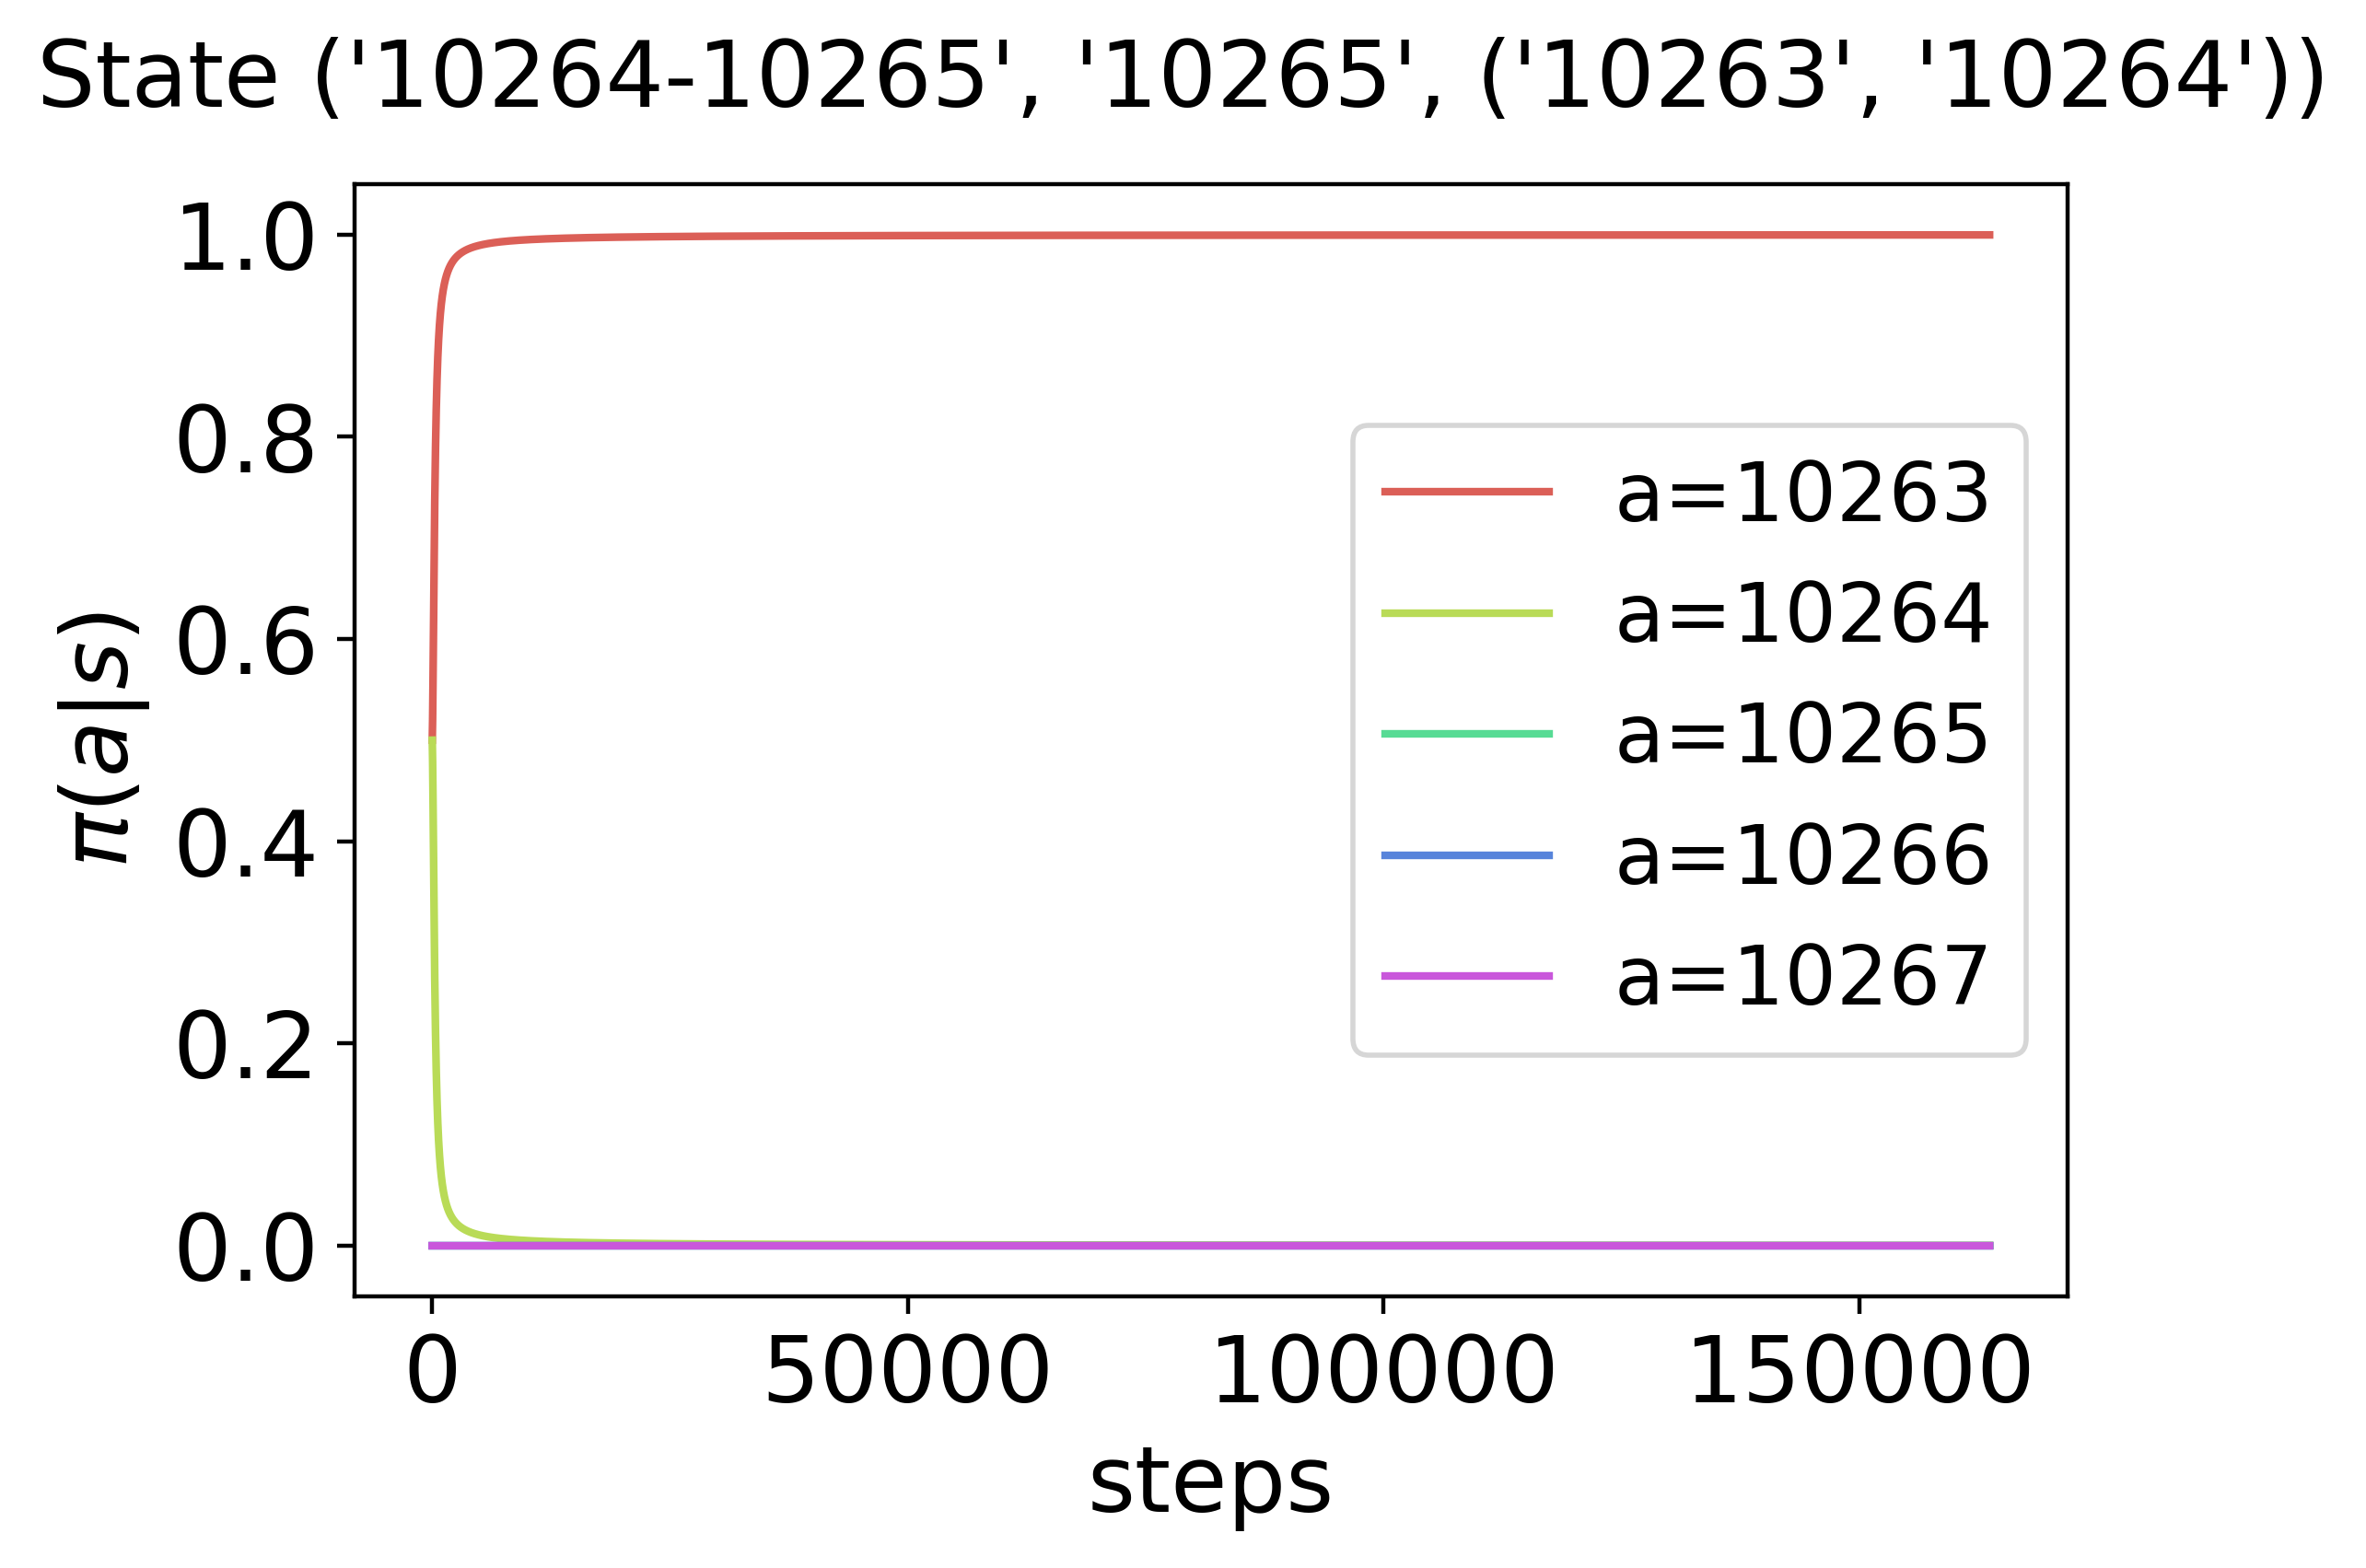
\includegraphics[scale=0.34,valign=b]{figures/policy_PG_state_1.png} \\
            \hspace*{-5pt}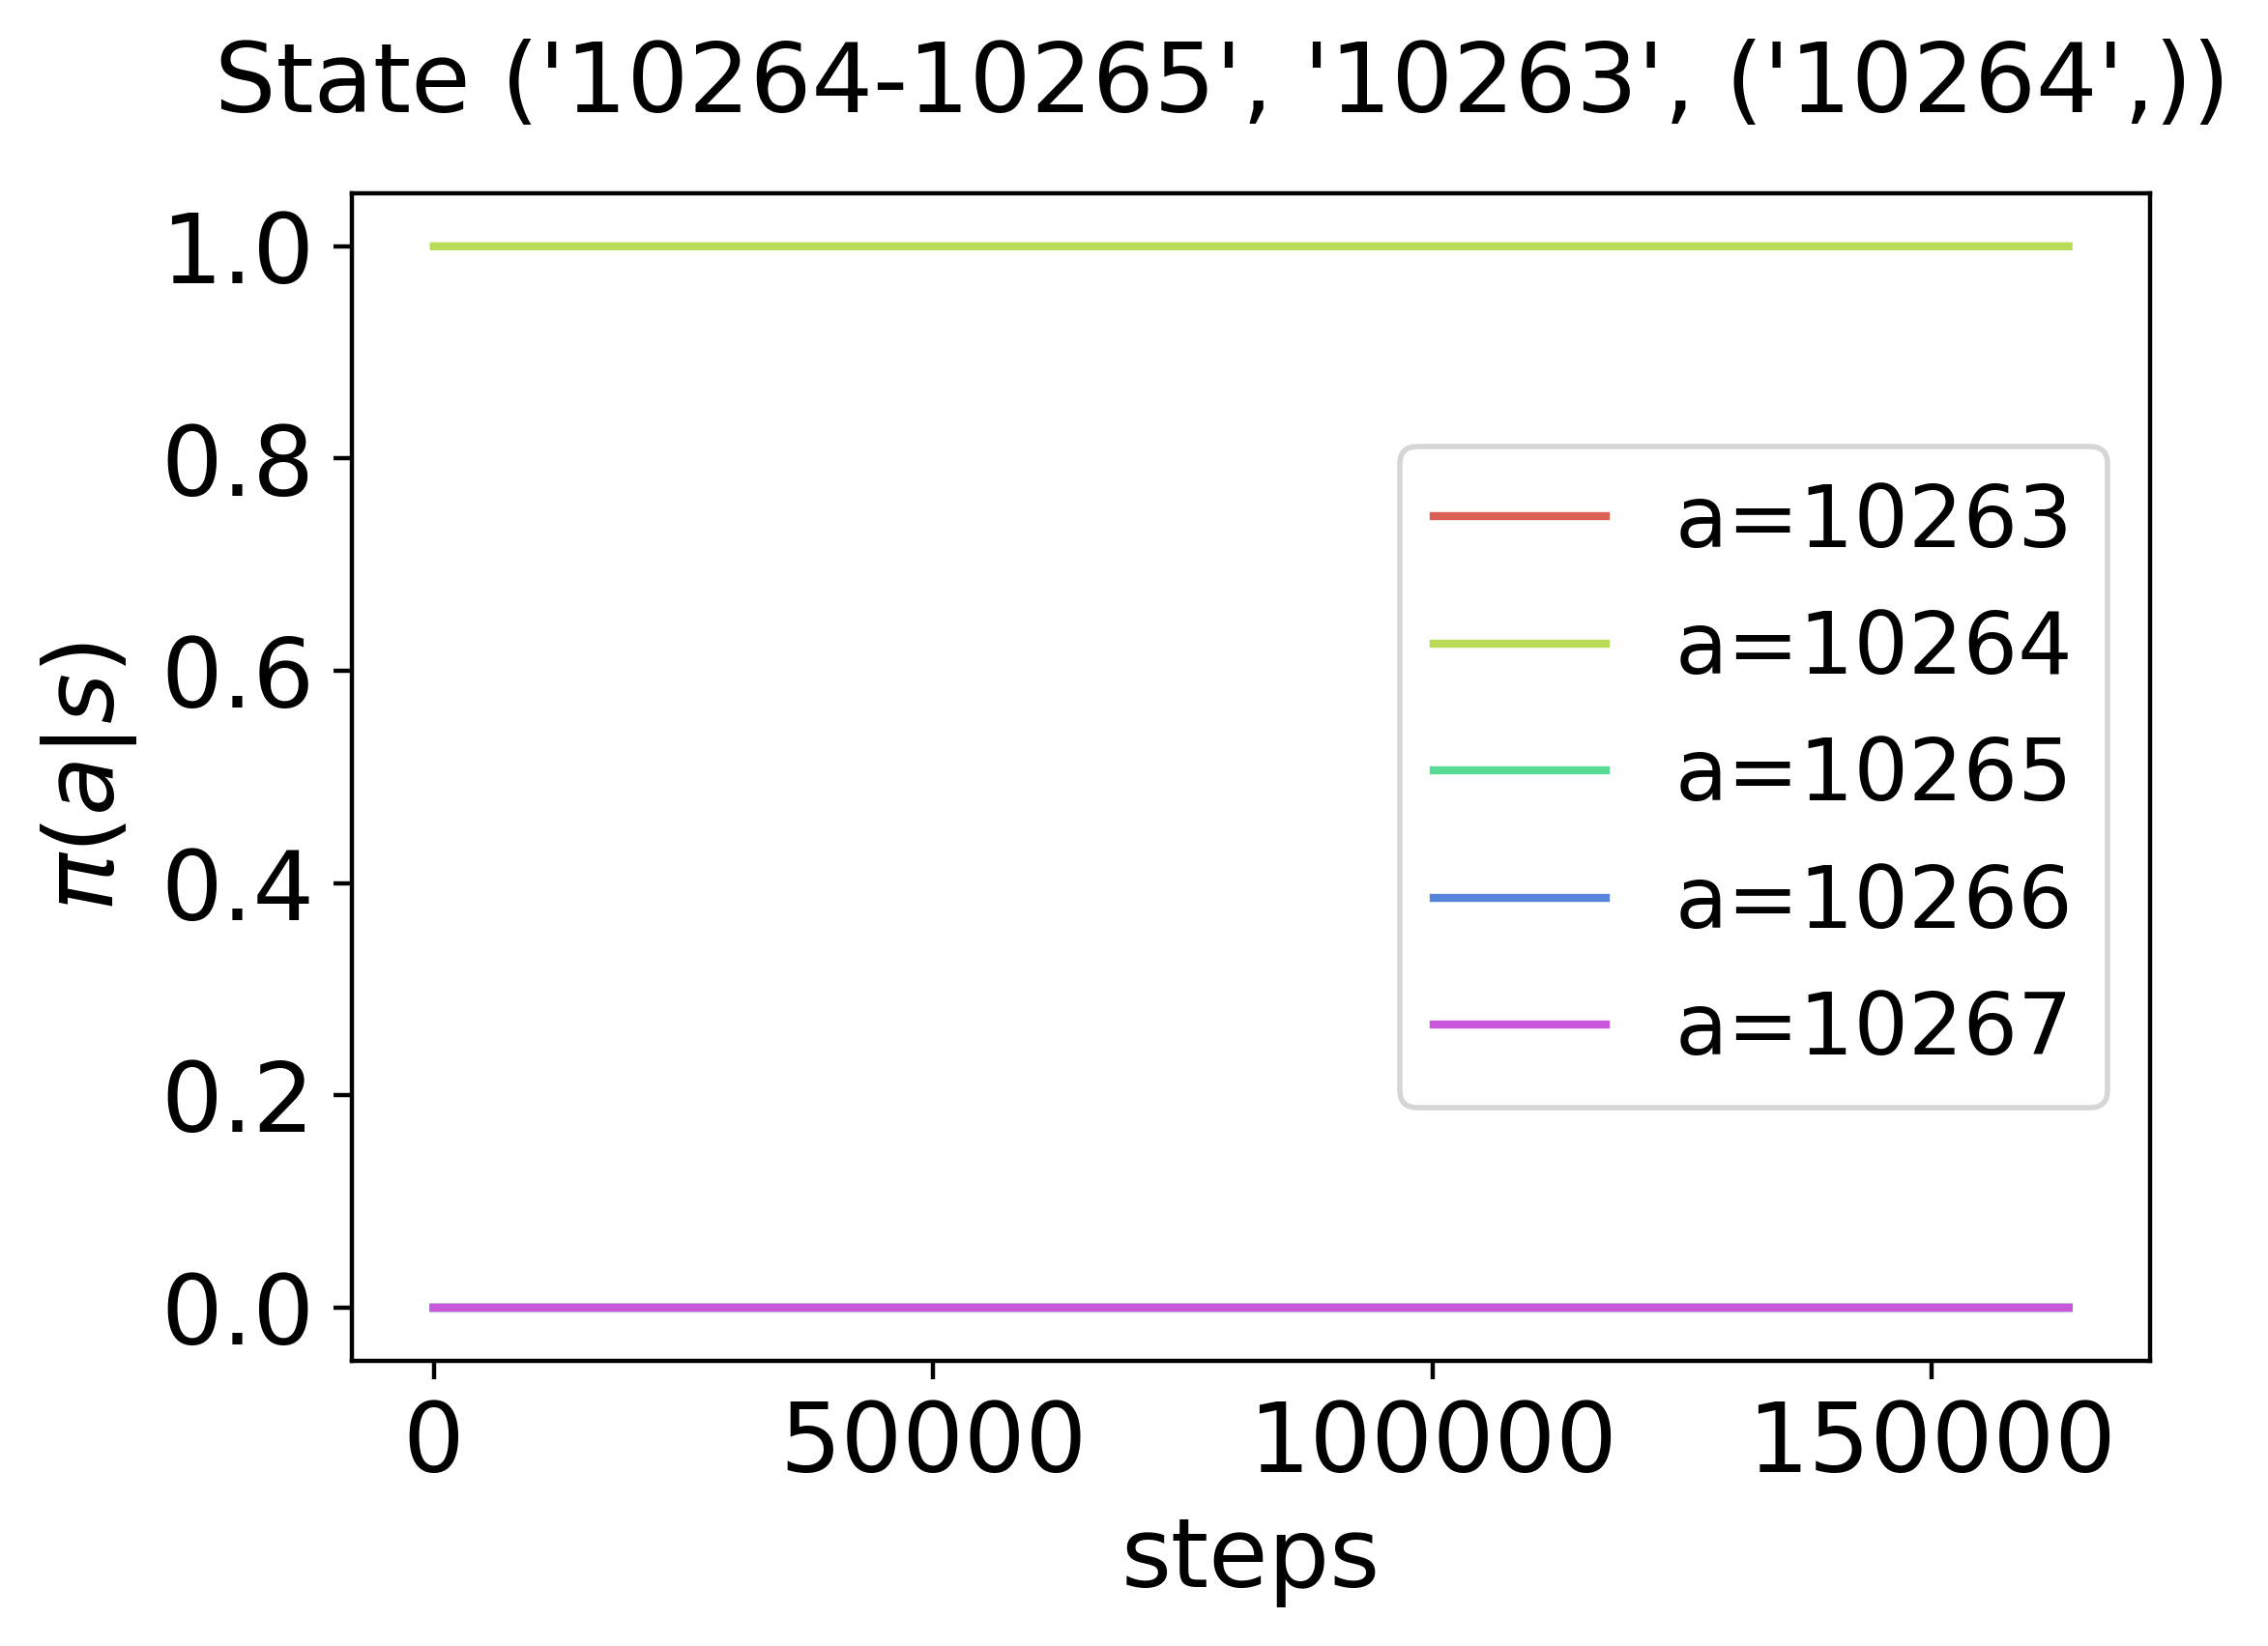
\includegraphics[scale=0.34,valign=b]{figures/policy_PG_state_2.png} &
            \hspace*{-18pt}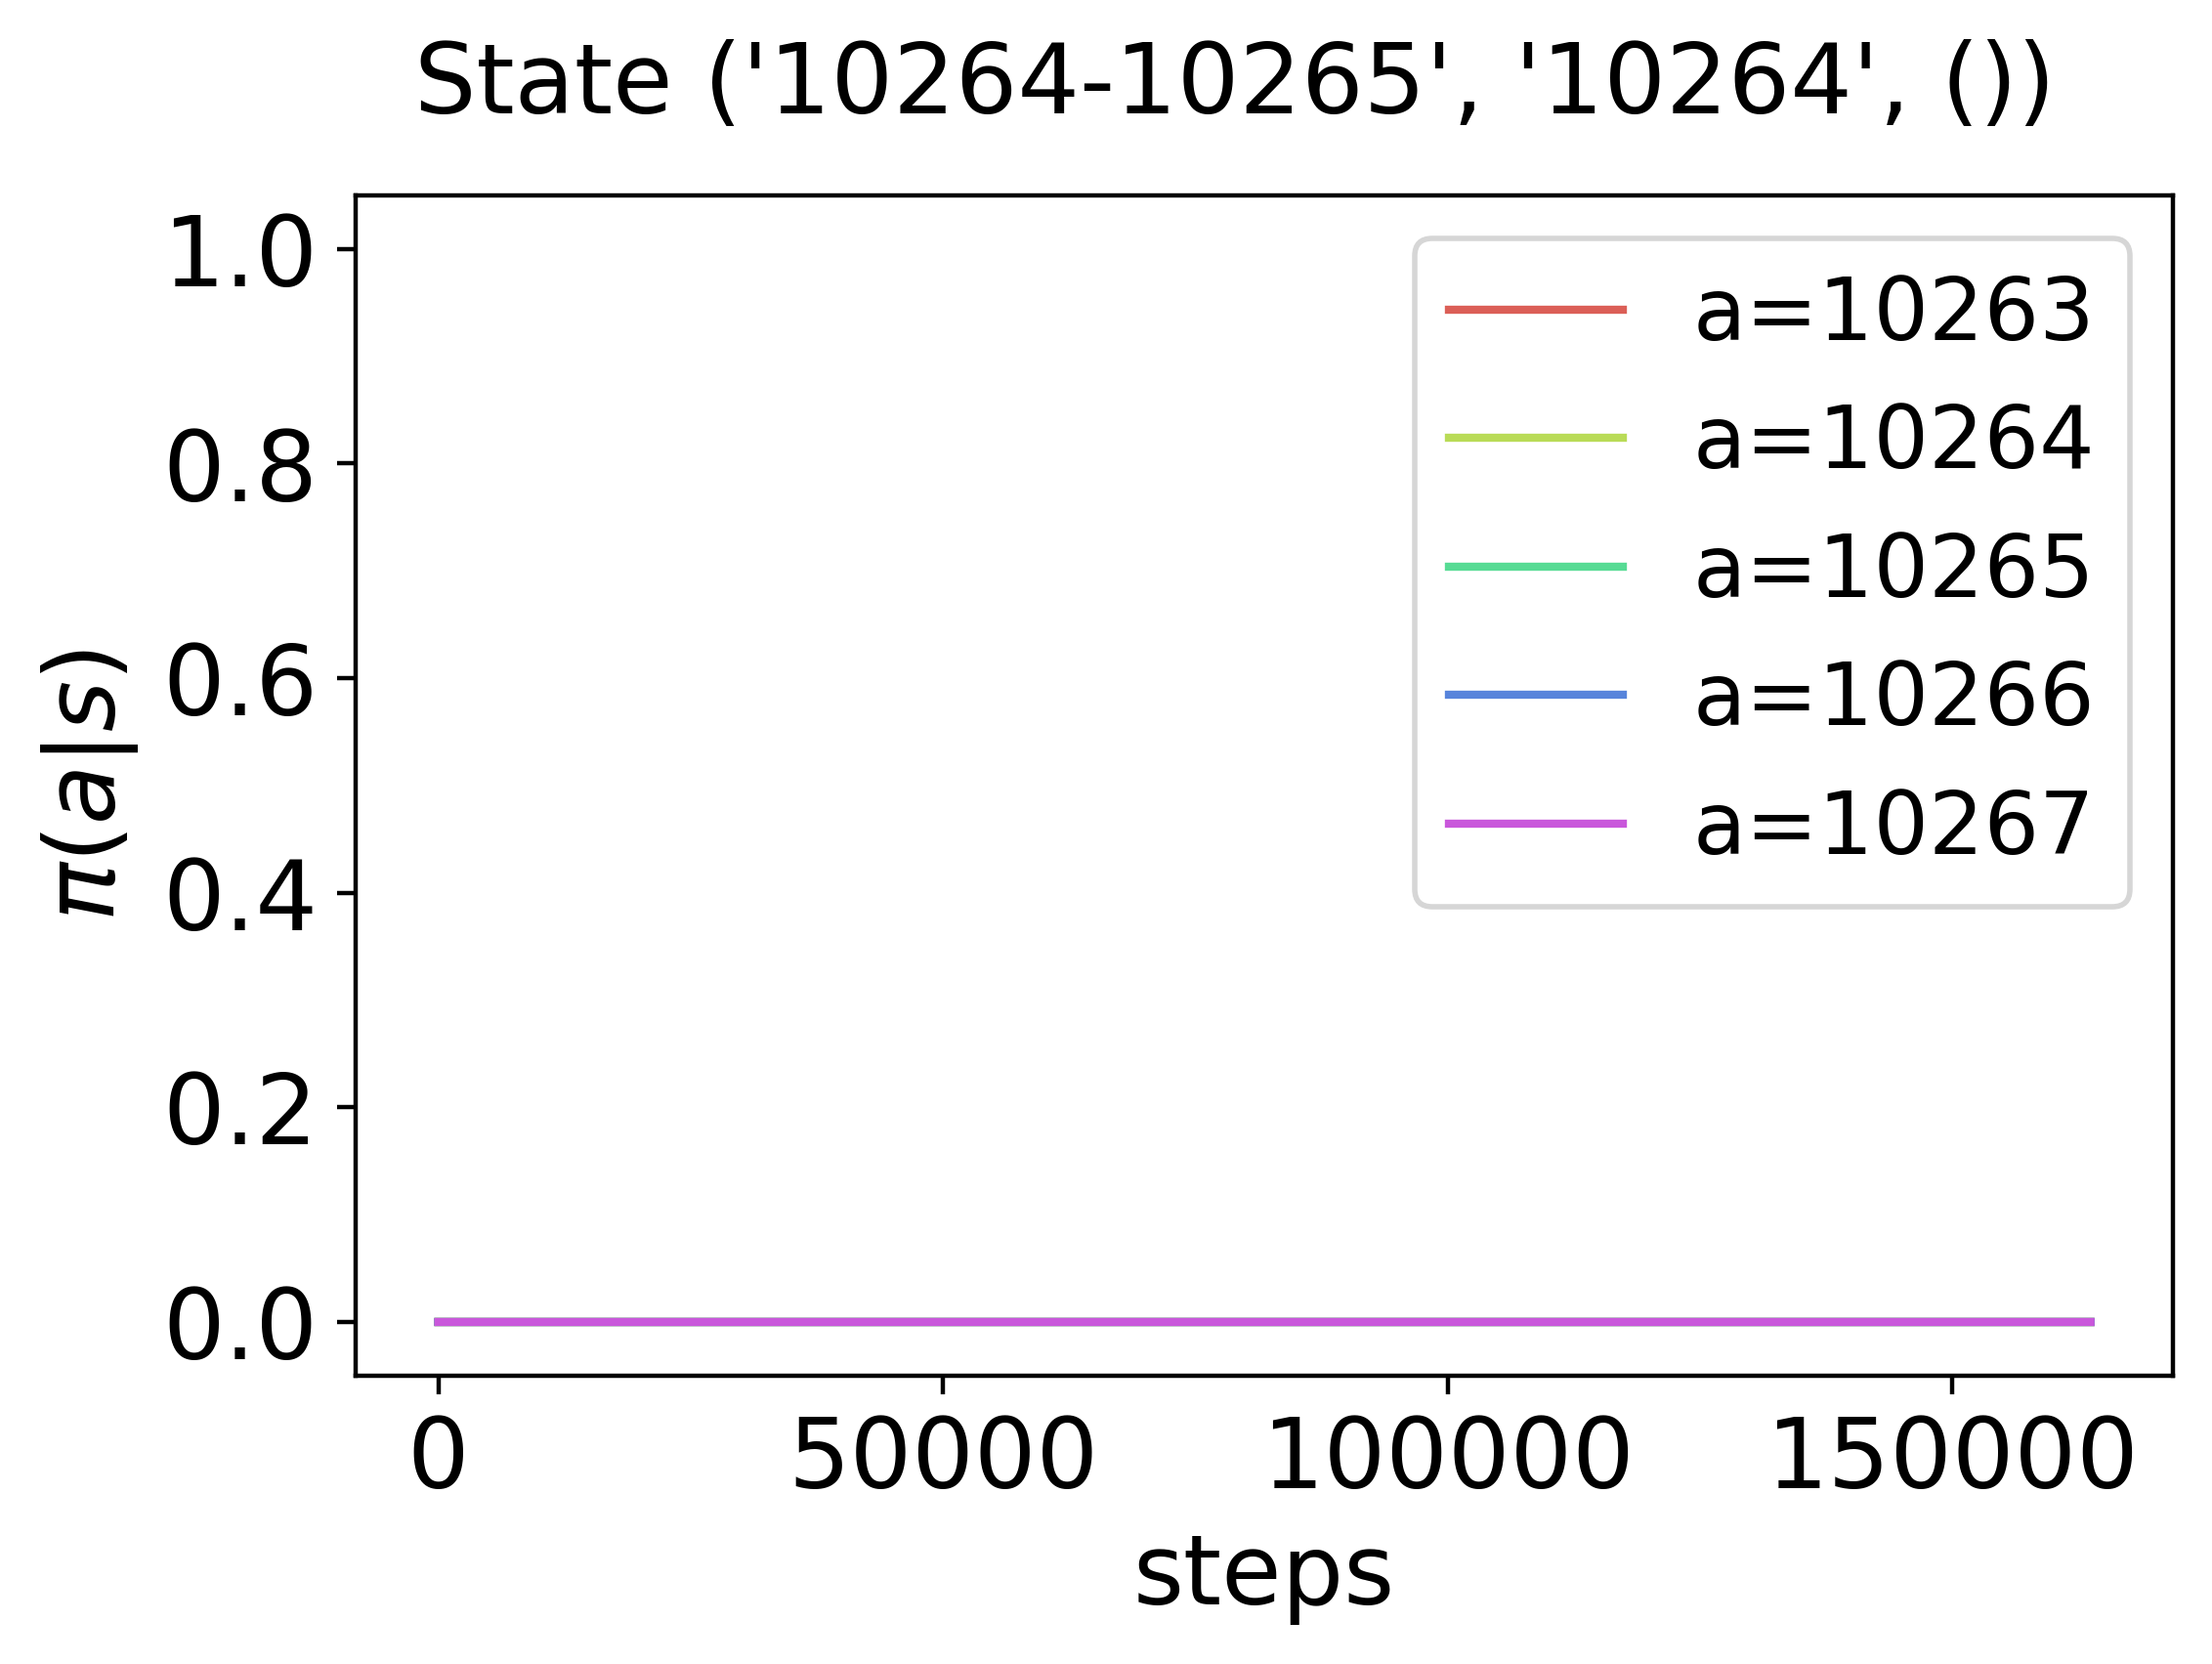
\includegraphics[scale=0.34,valign=b]{figures/policy_PG_state_3.png}
        \end{tabular}
    \end{figure}
    
\end{frame}

\begin{frame}{Trajectories of the parameters $\boldsymbol \theta$ for NPG}

    \begin{figure}
        \centering
        \begin{tabular}{cc}
            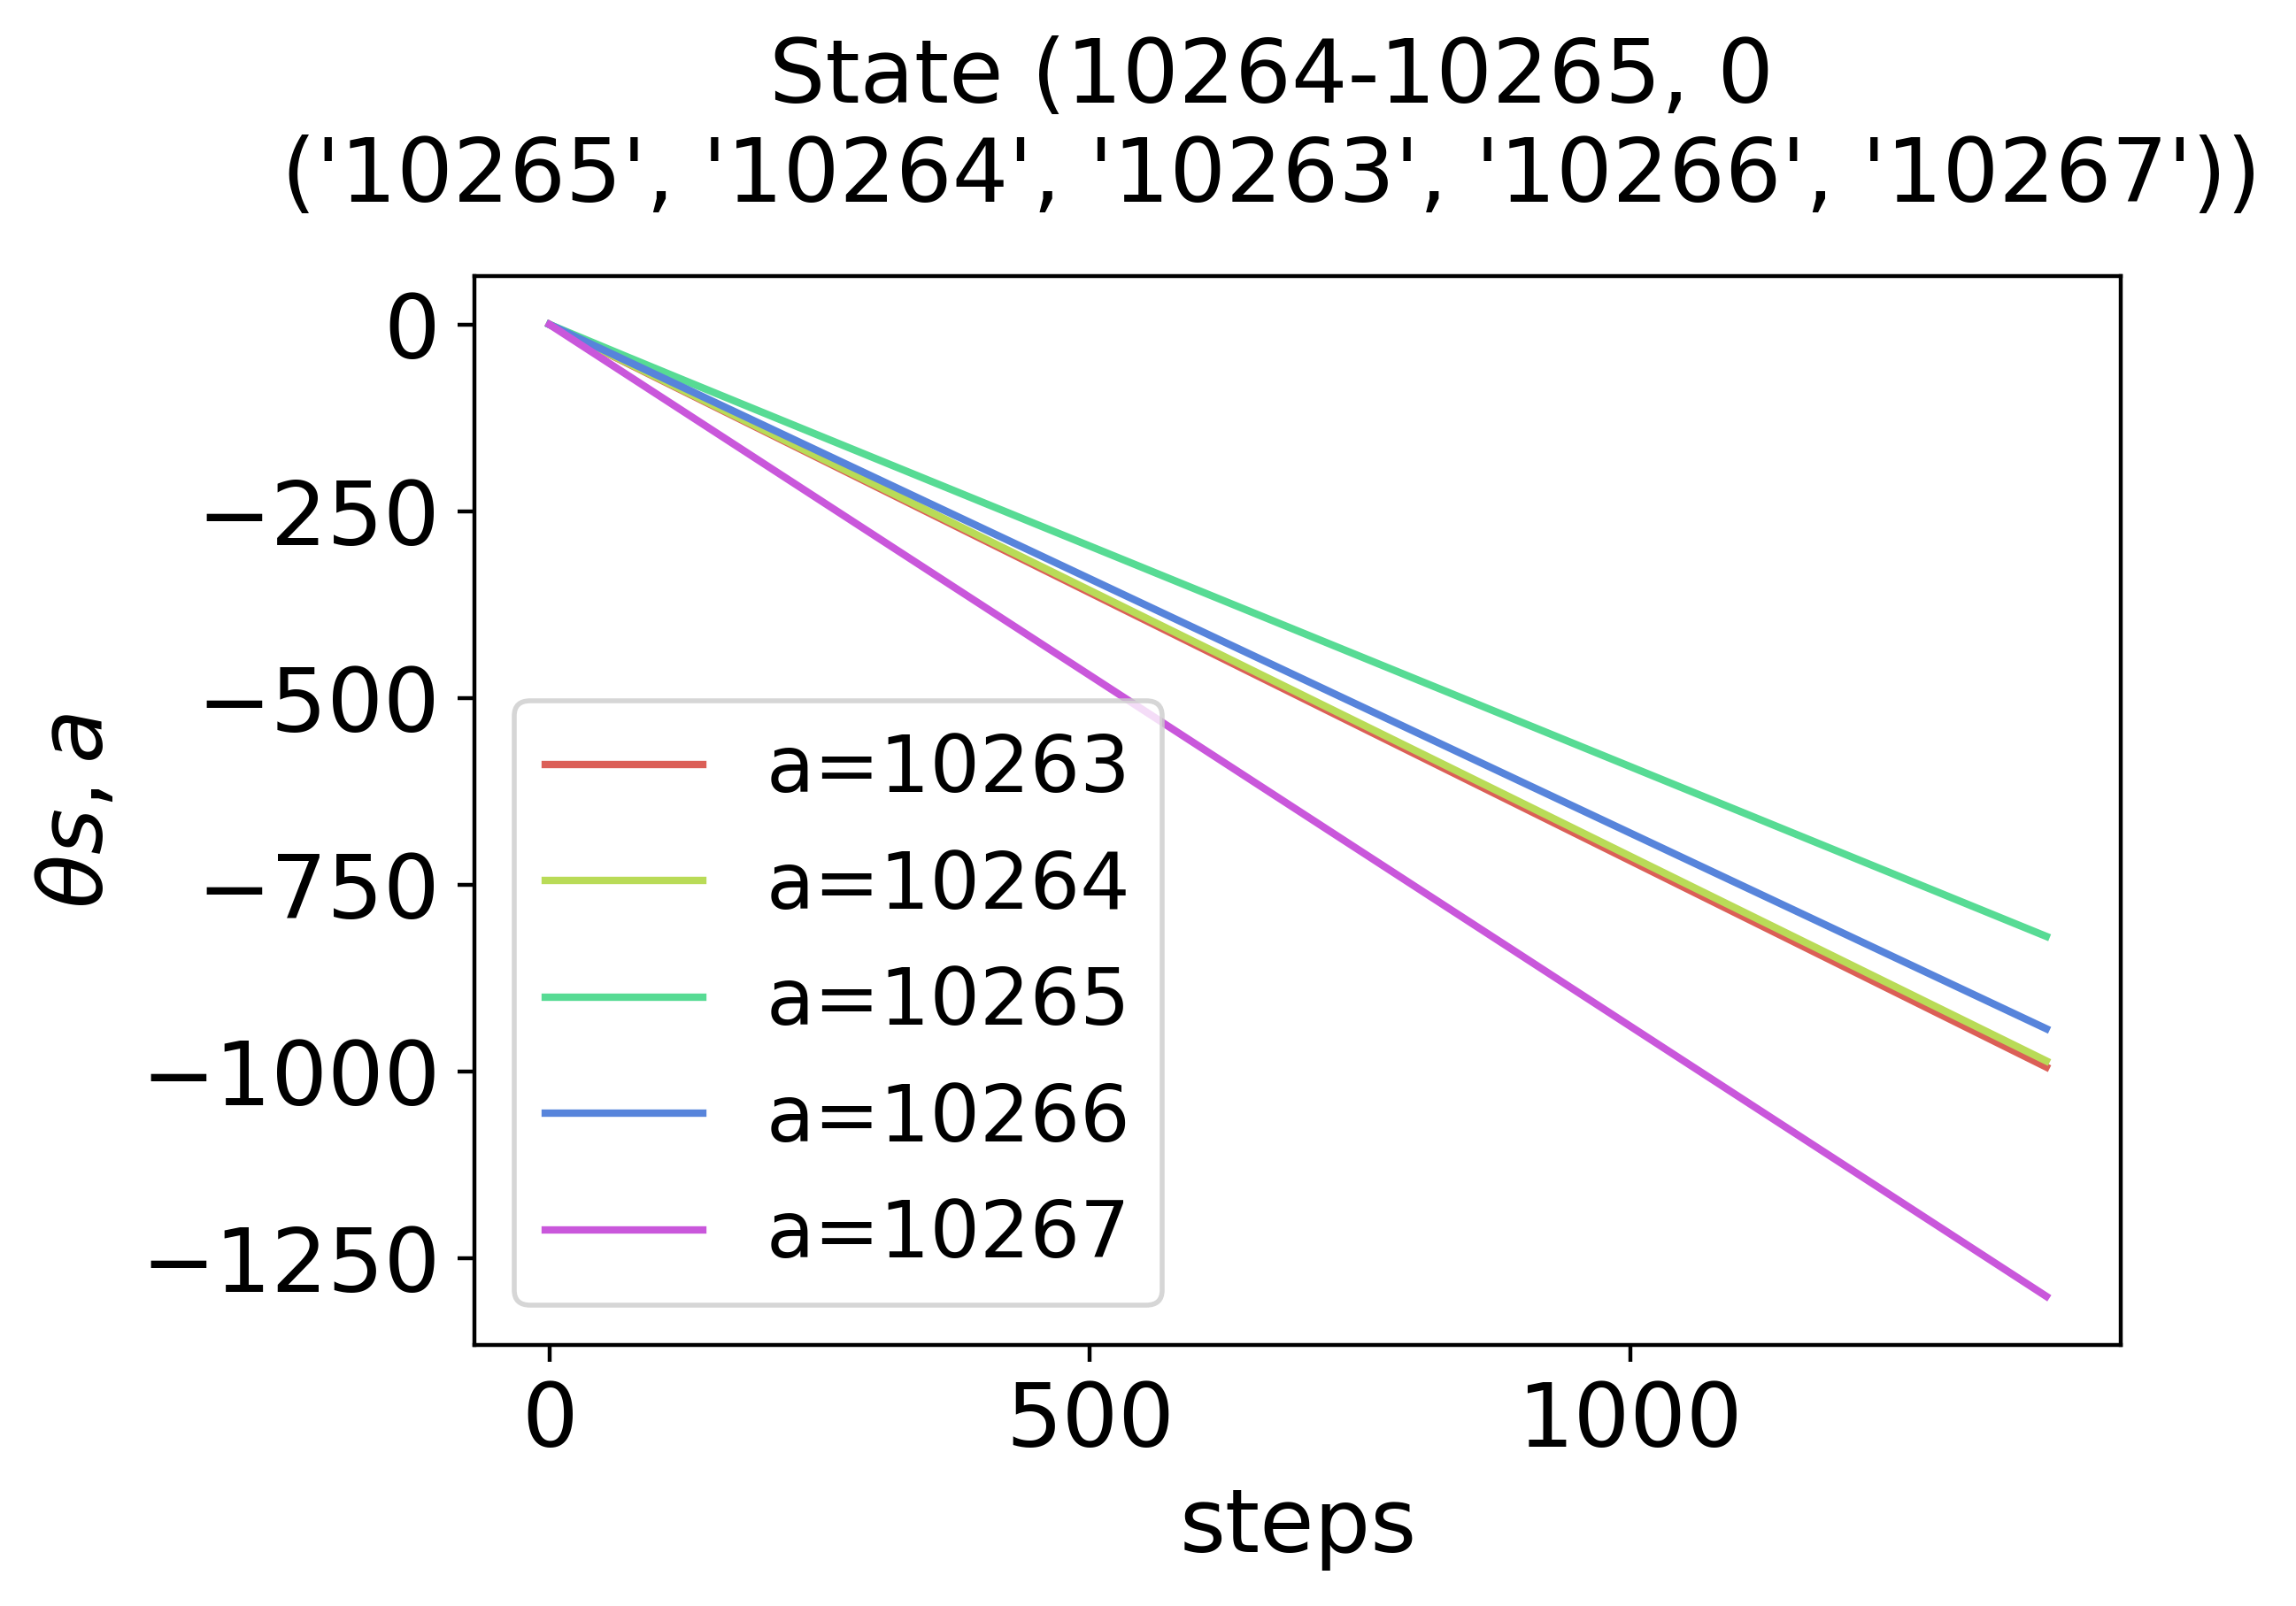
\includegraphics[scale=0.34,valign=b]{figures/theta_NPG_state_0.png} &
            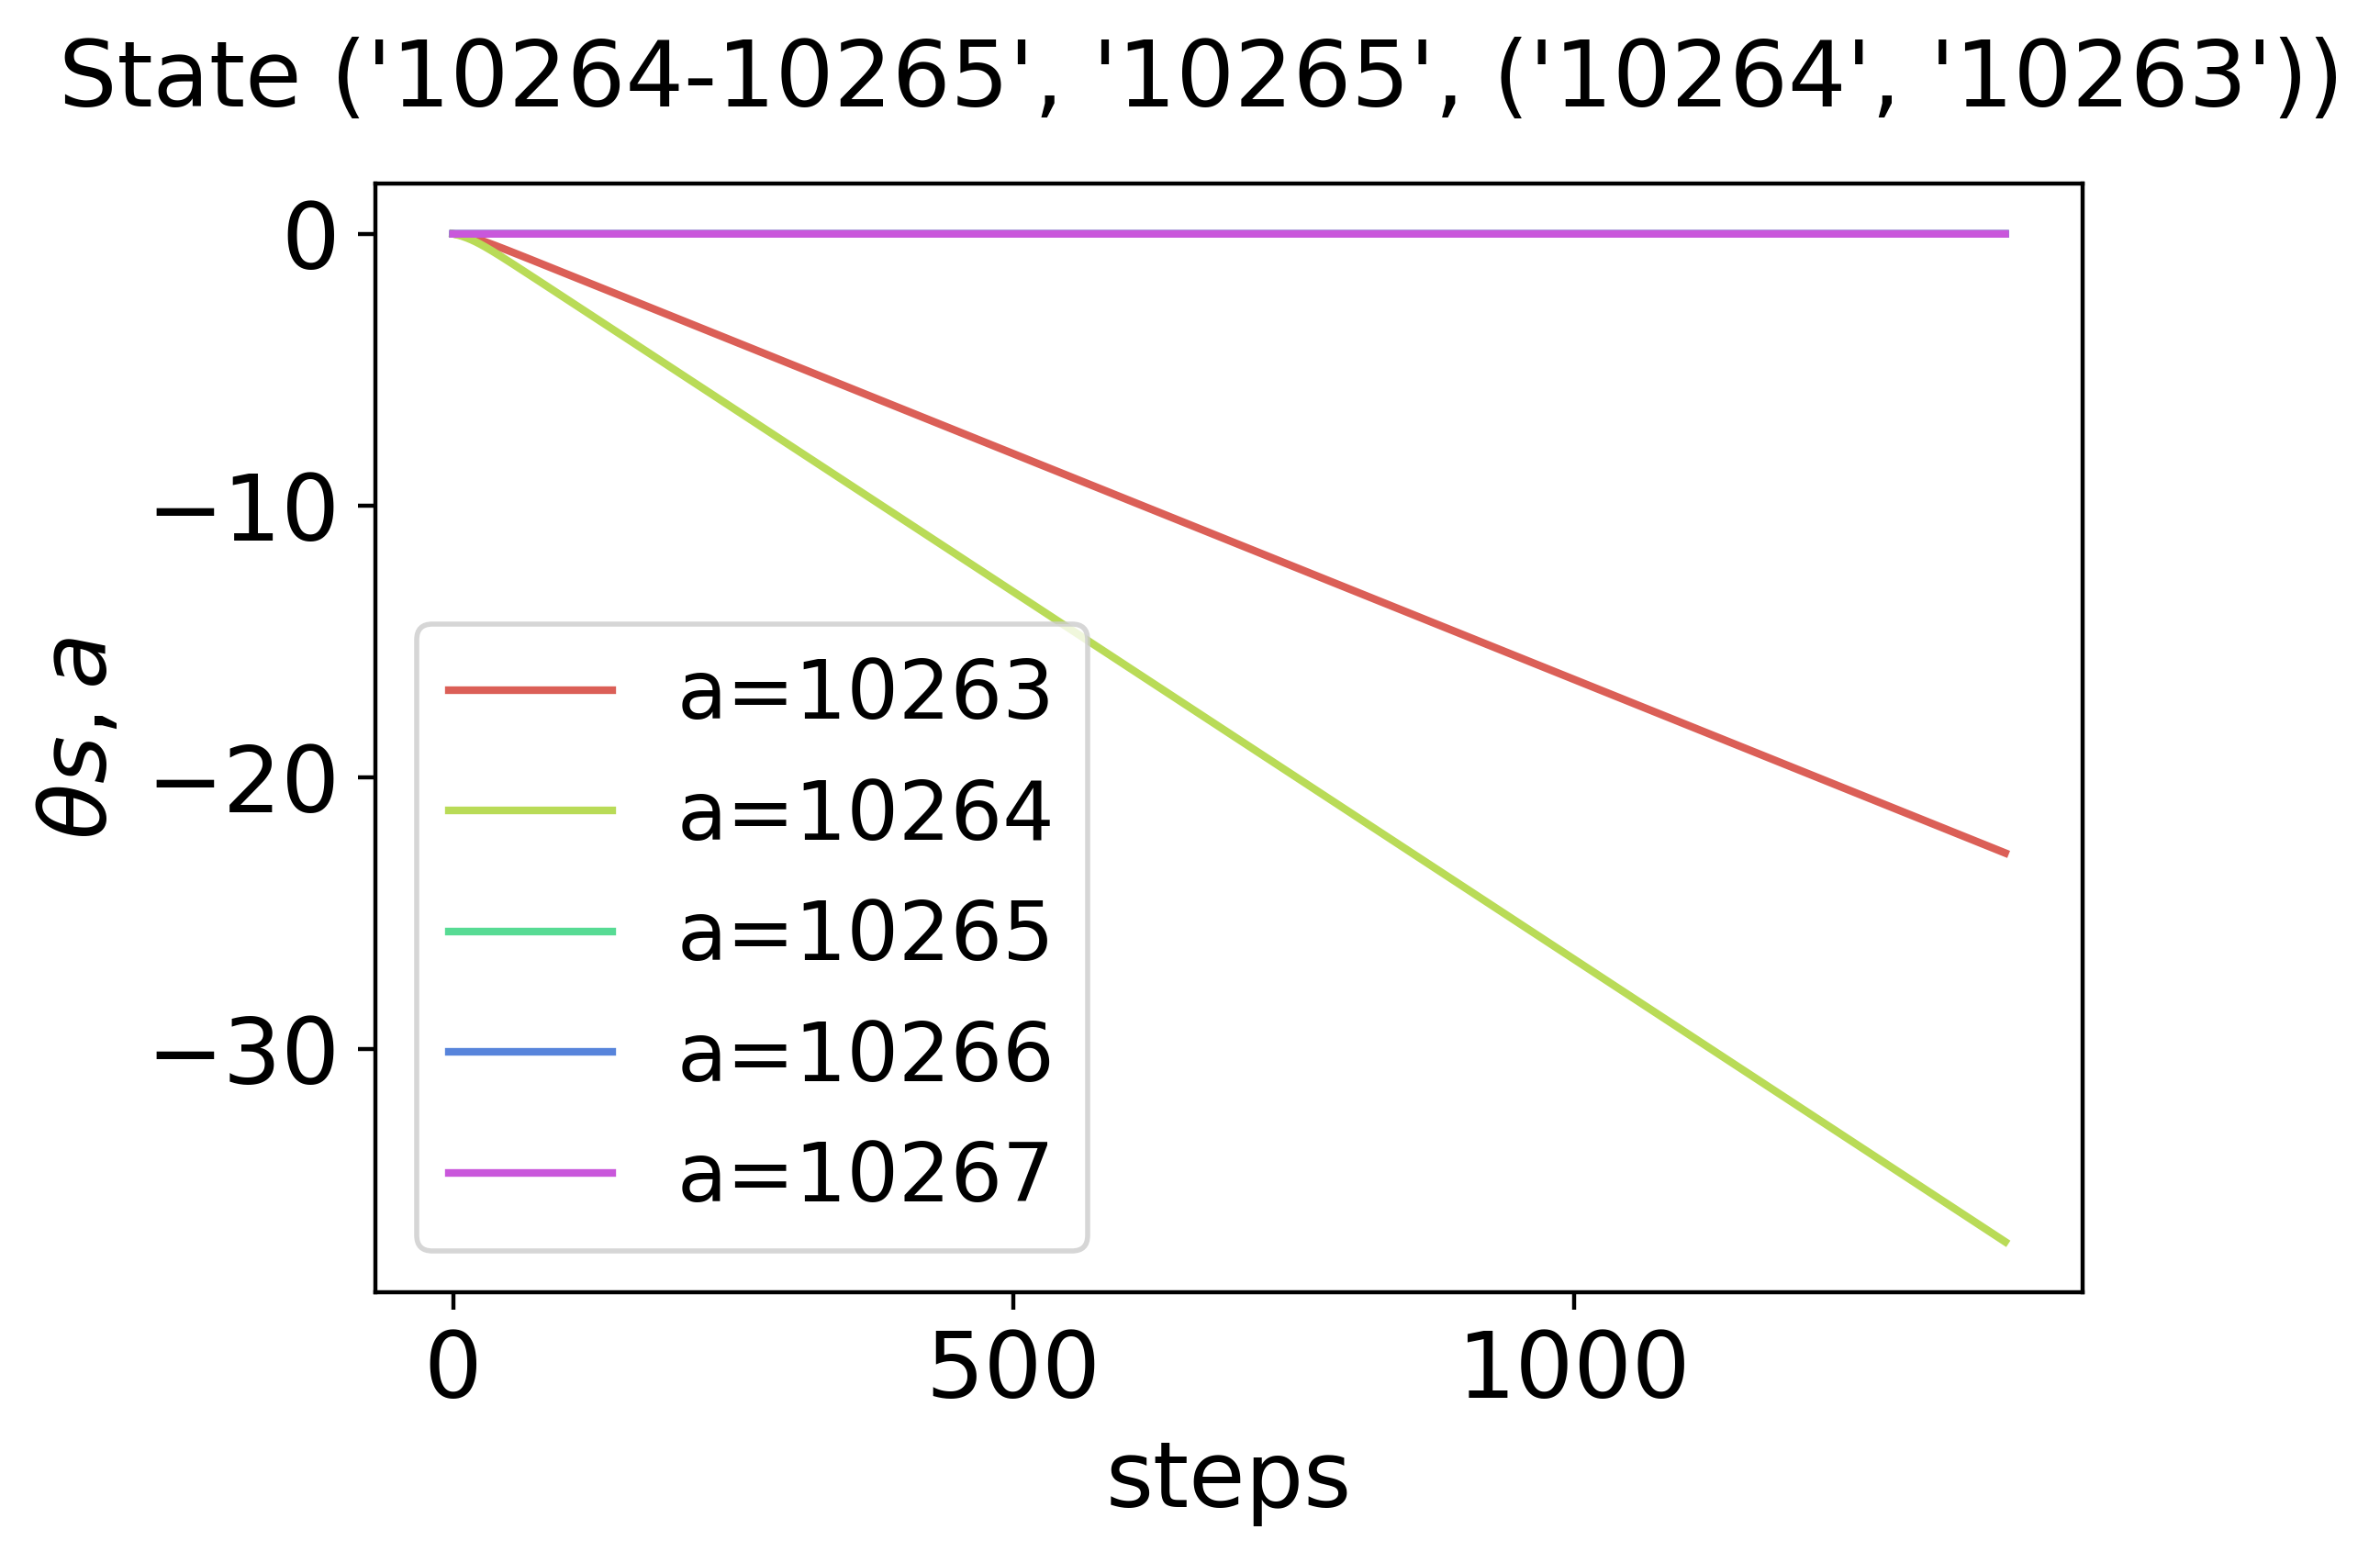
\includegraphics[scale=0.34,valign=b]{figures/theta_NPG_state_1.png} \\
            \hspace*{9pt}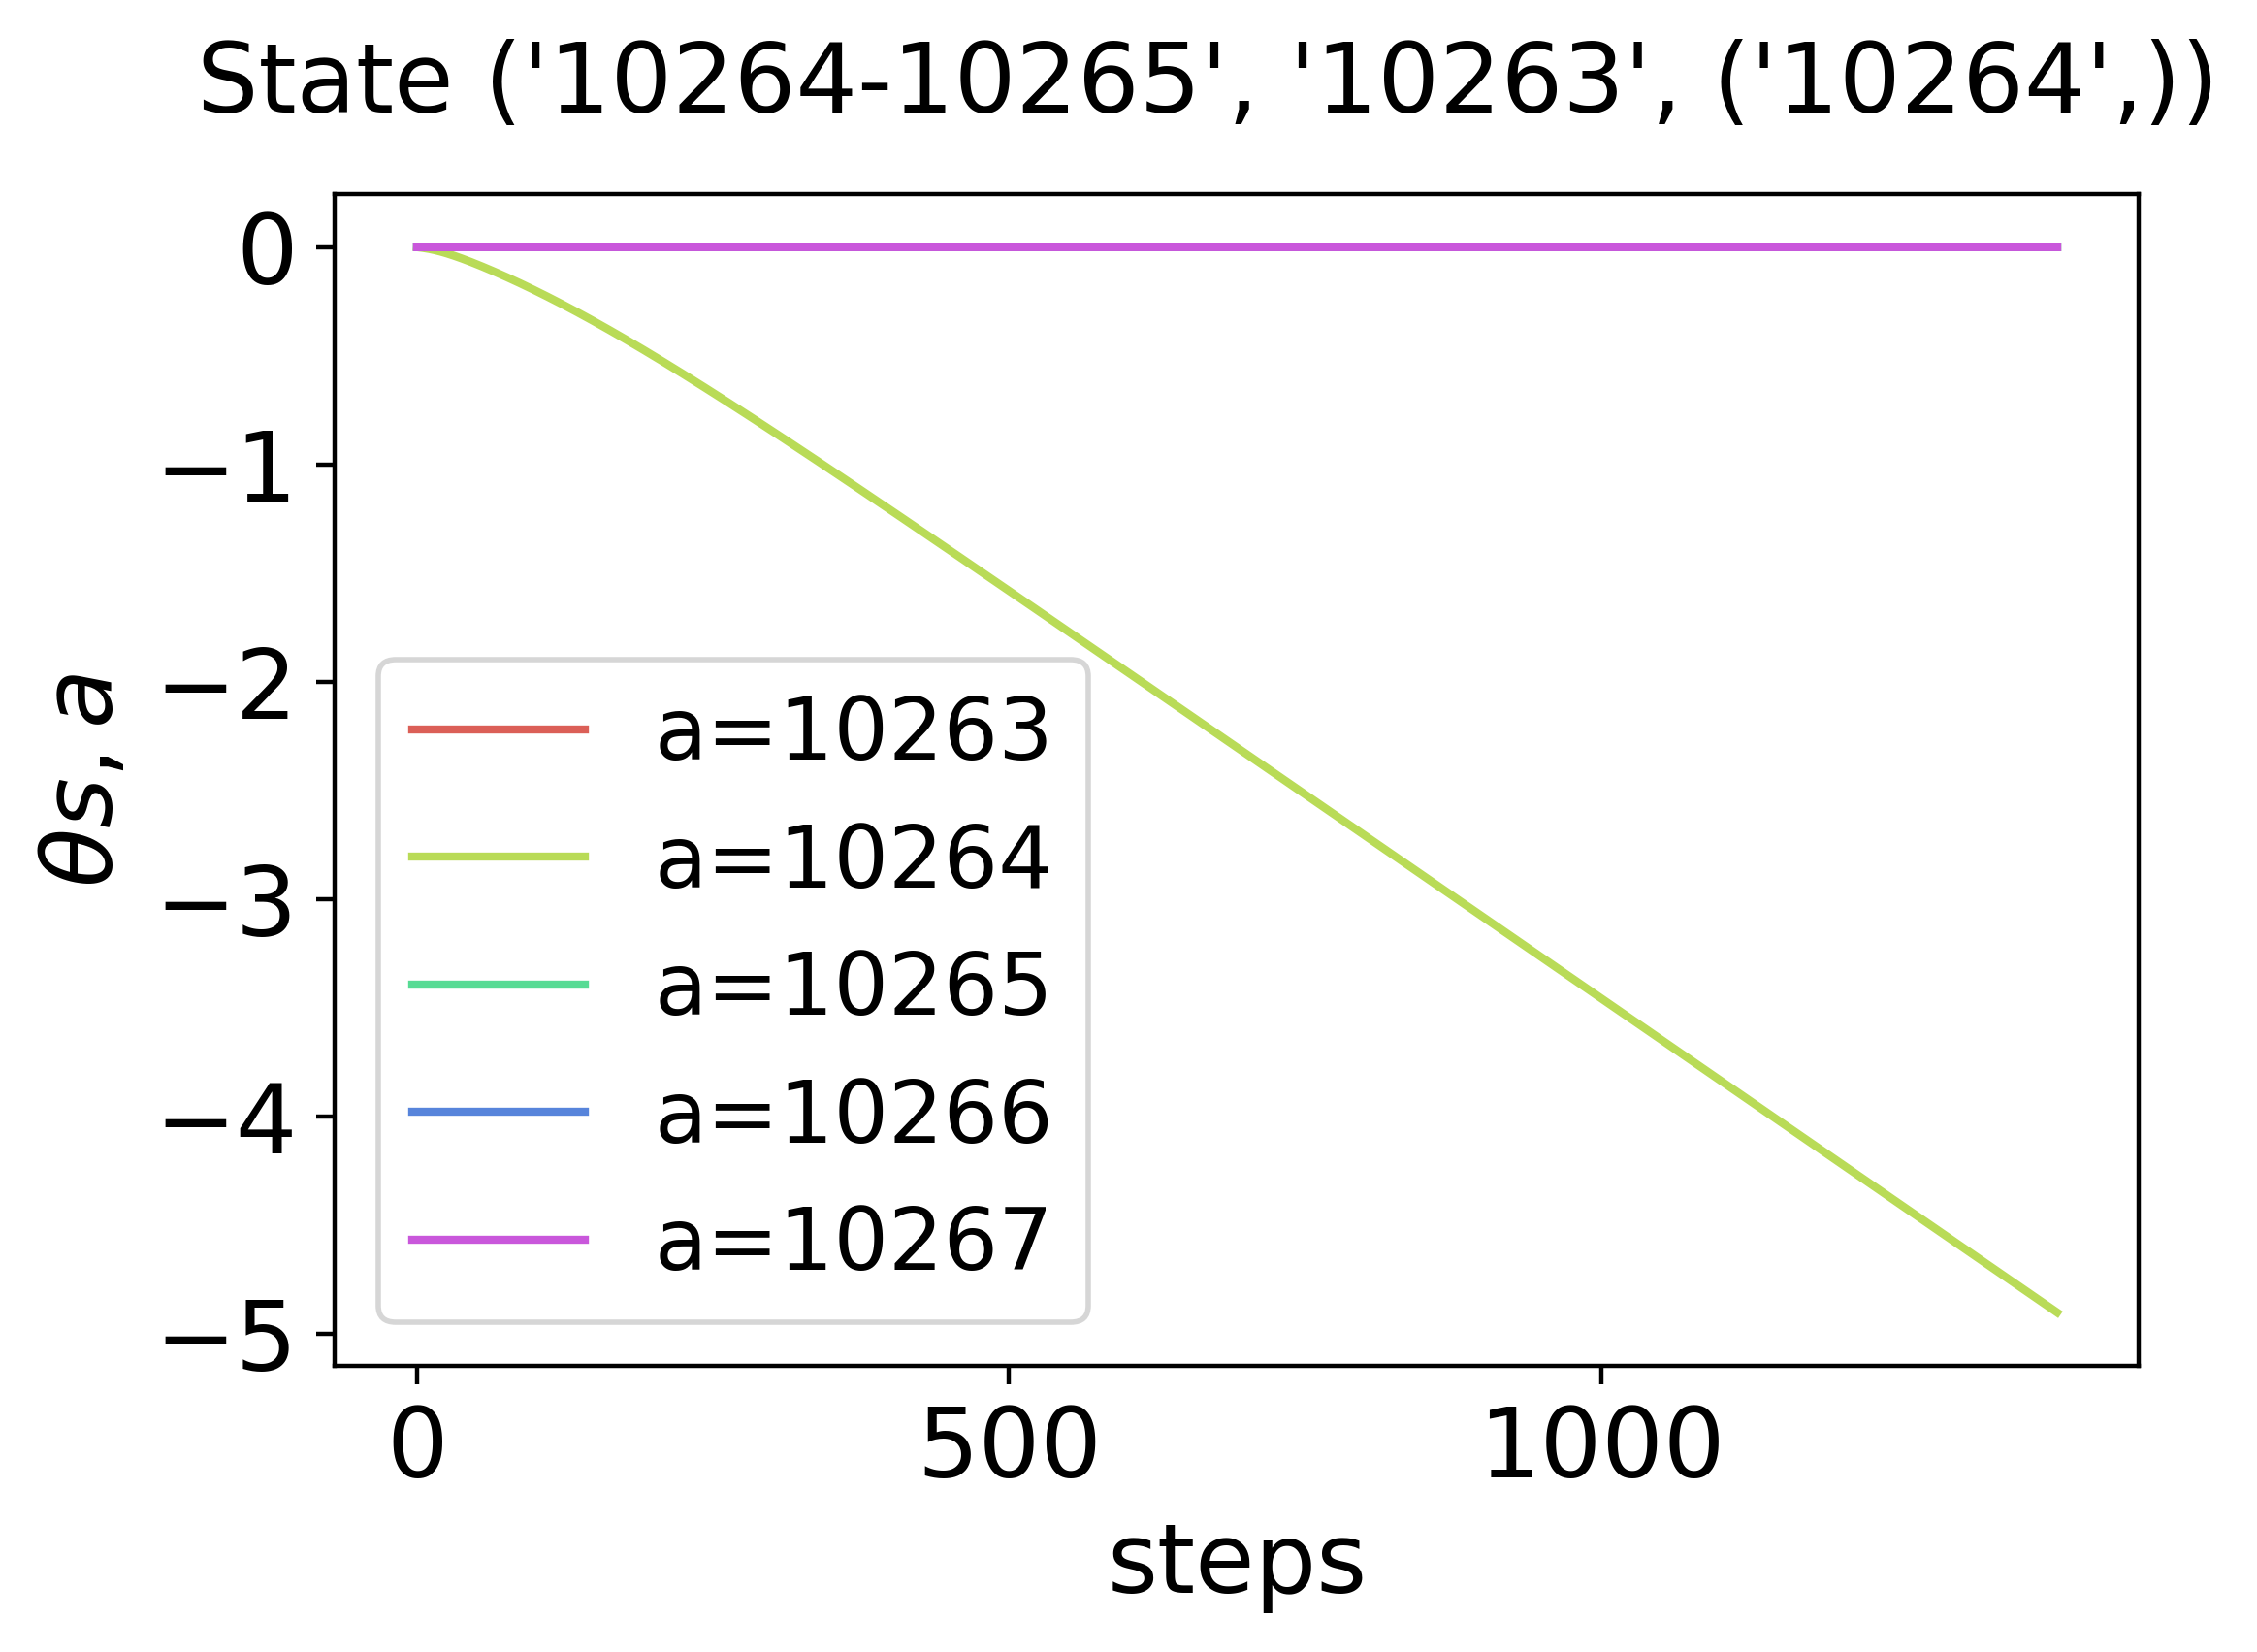
\includegraphics[scale=0.34,valign=b]{figures/theta_NPG_state_2.png} &
            \hspace*{-26.7pt}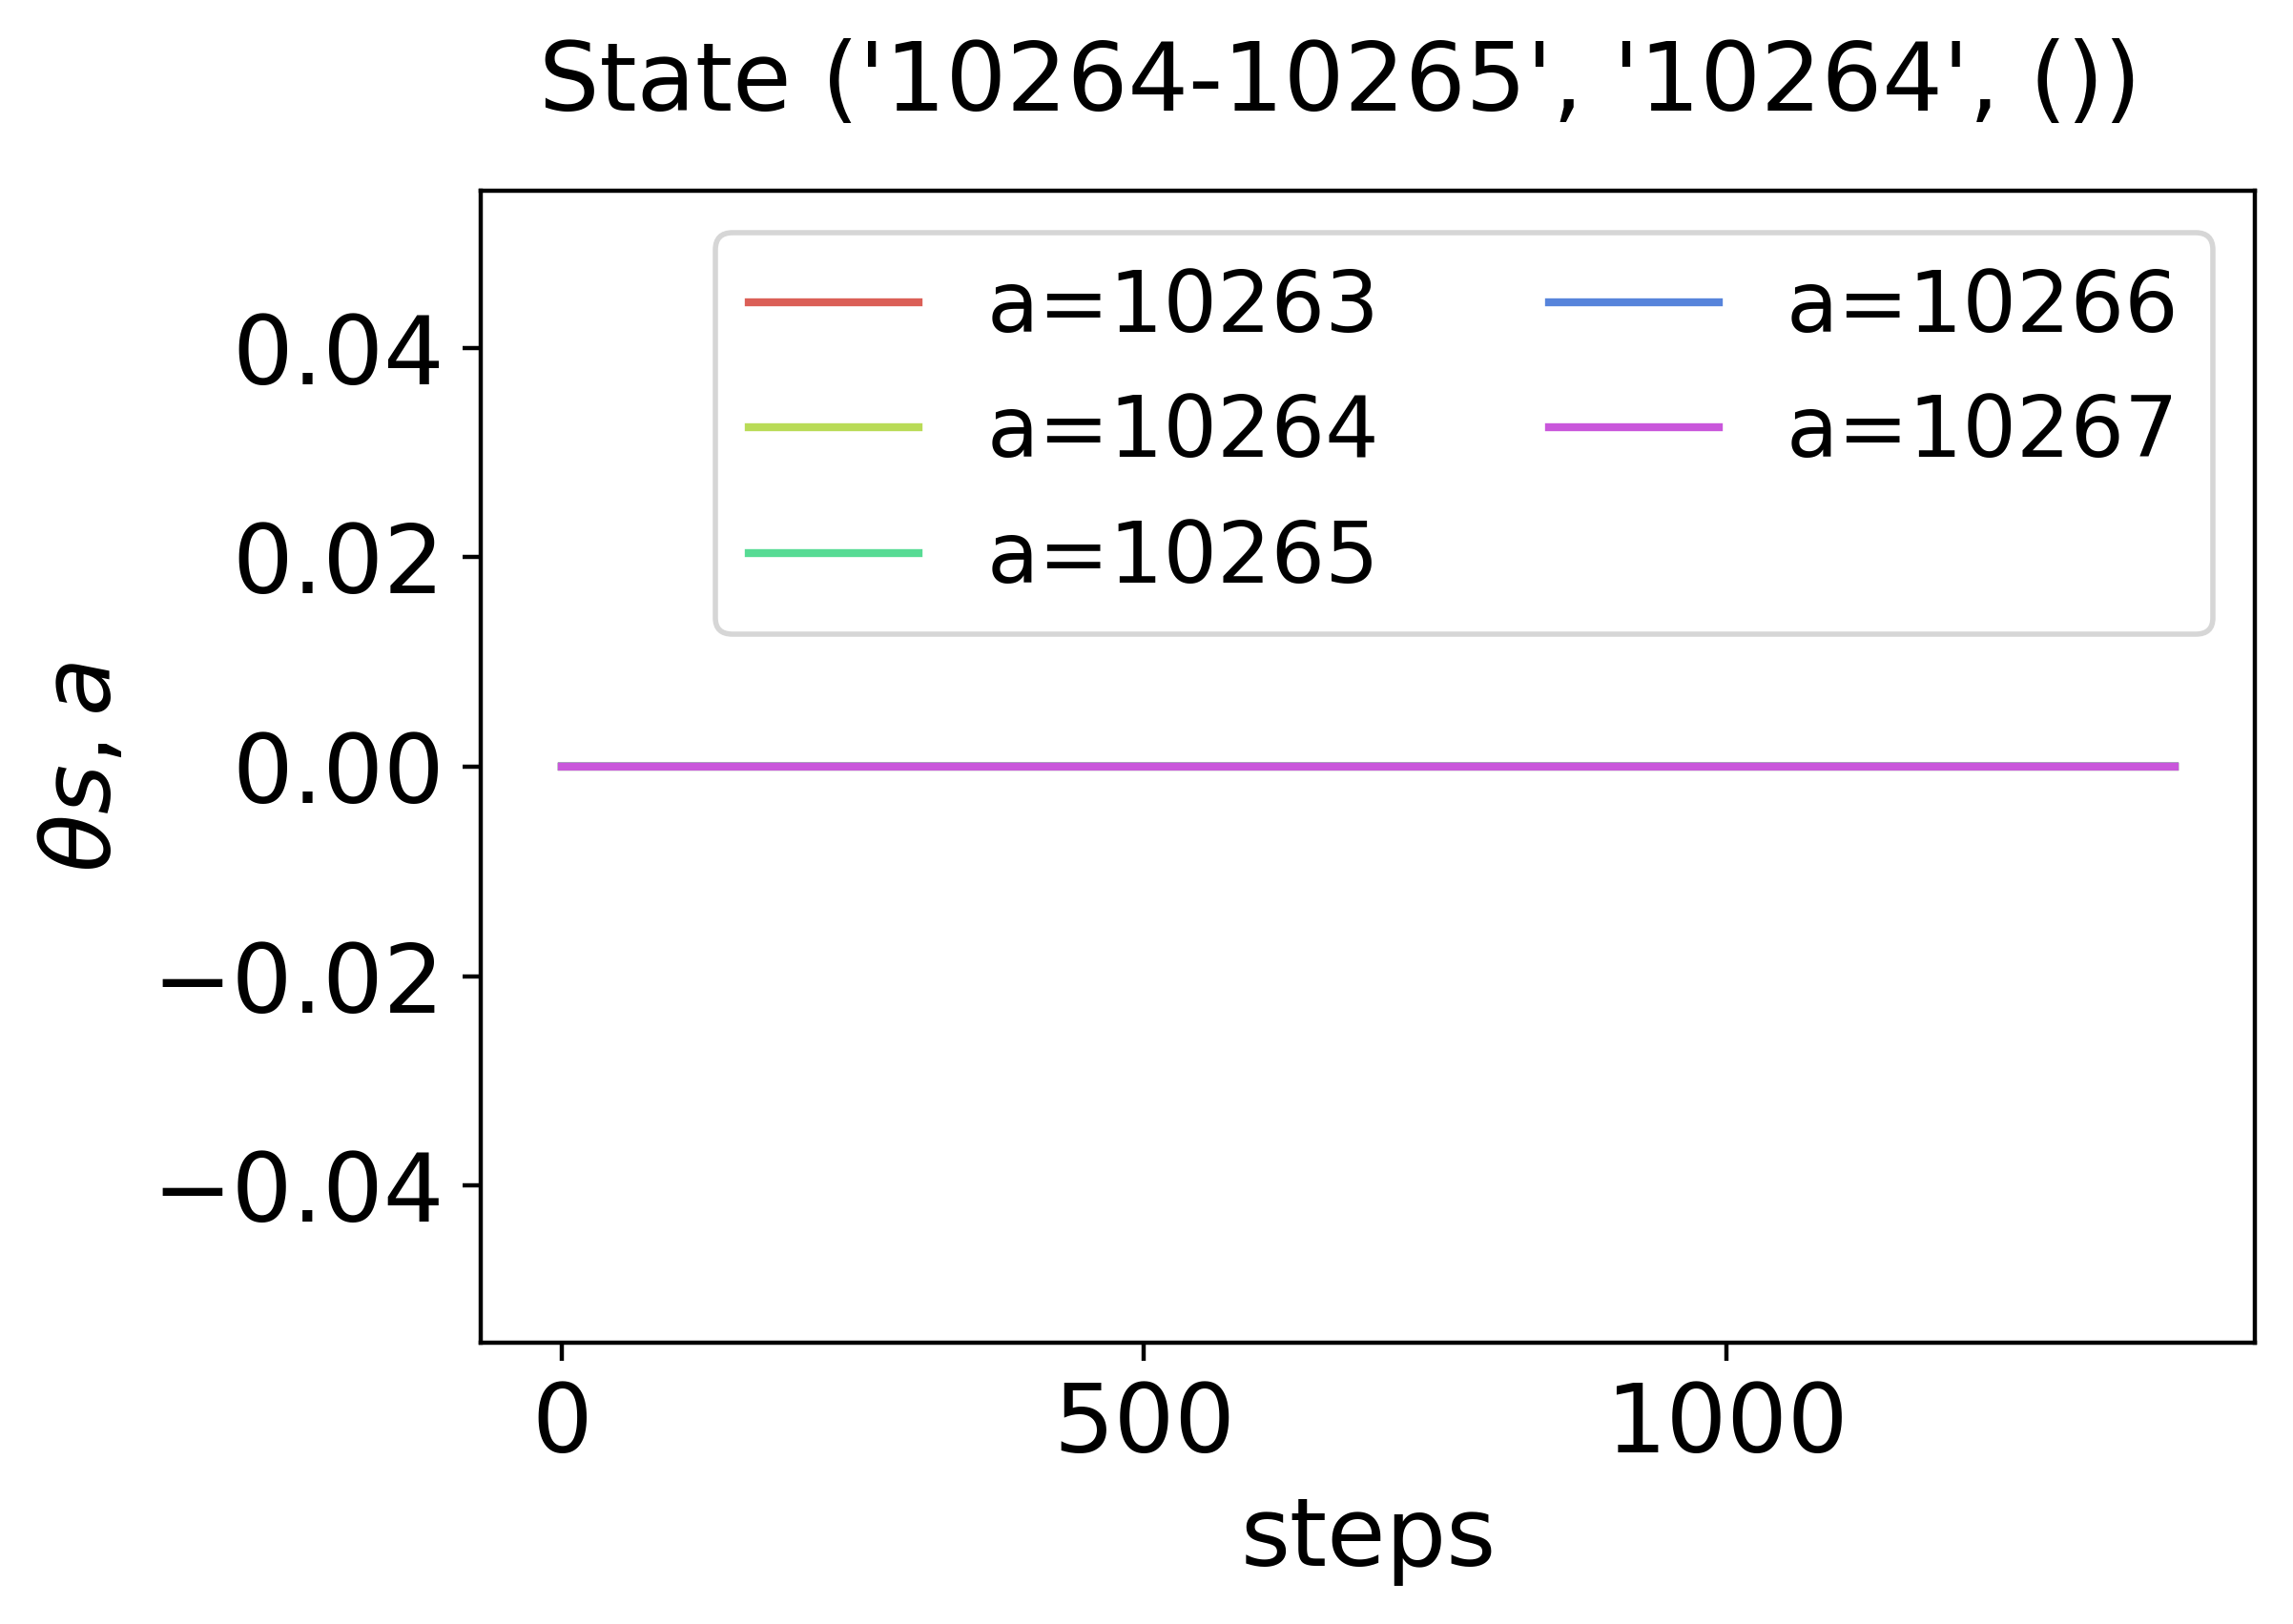
\includegraphics[scale=0.34,valign=b]{figures/theta_NPG_state_3.png}
        \end{tabular}
    \end{figure}
    
\end{frame}

\begin{frame}{Trajectories of the policies $\pi_{\boldsymbol \theta}$ for NPG}

    \begin{figure}
        \centering
        \begin{tabular}{cc}
            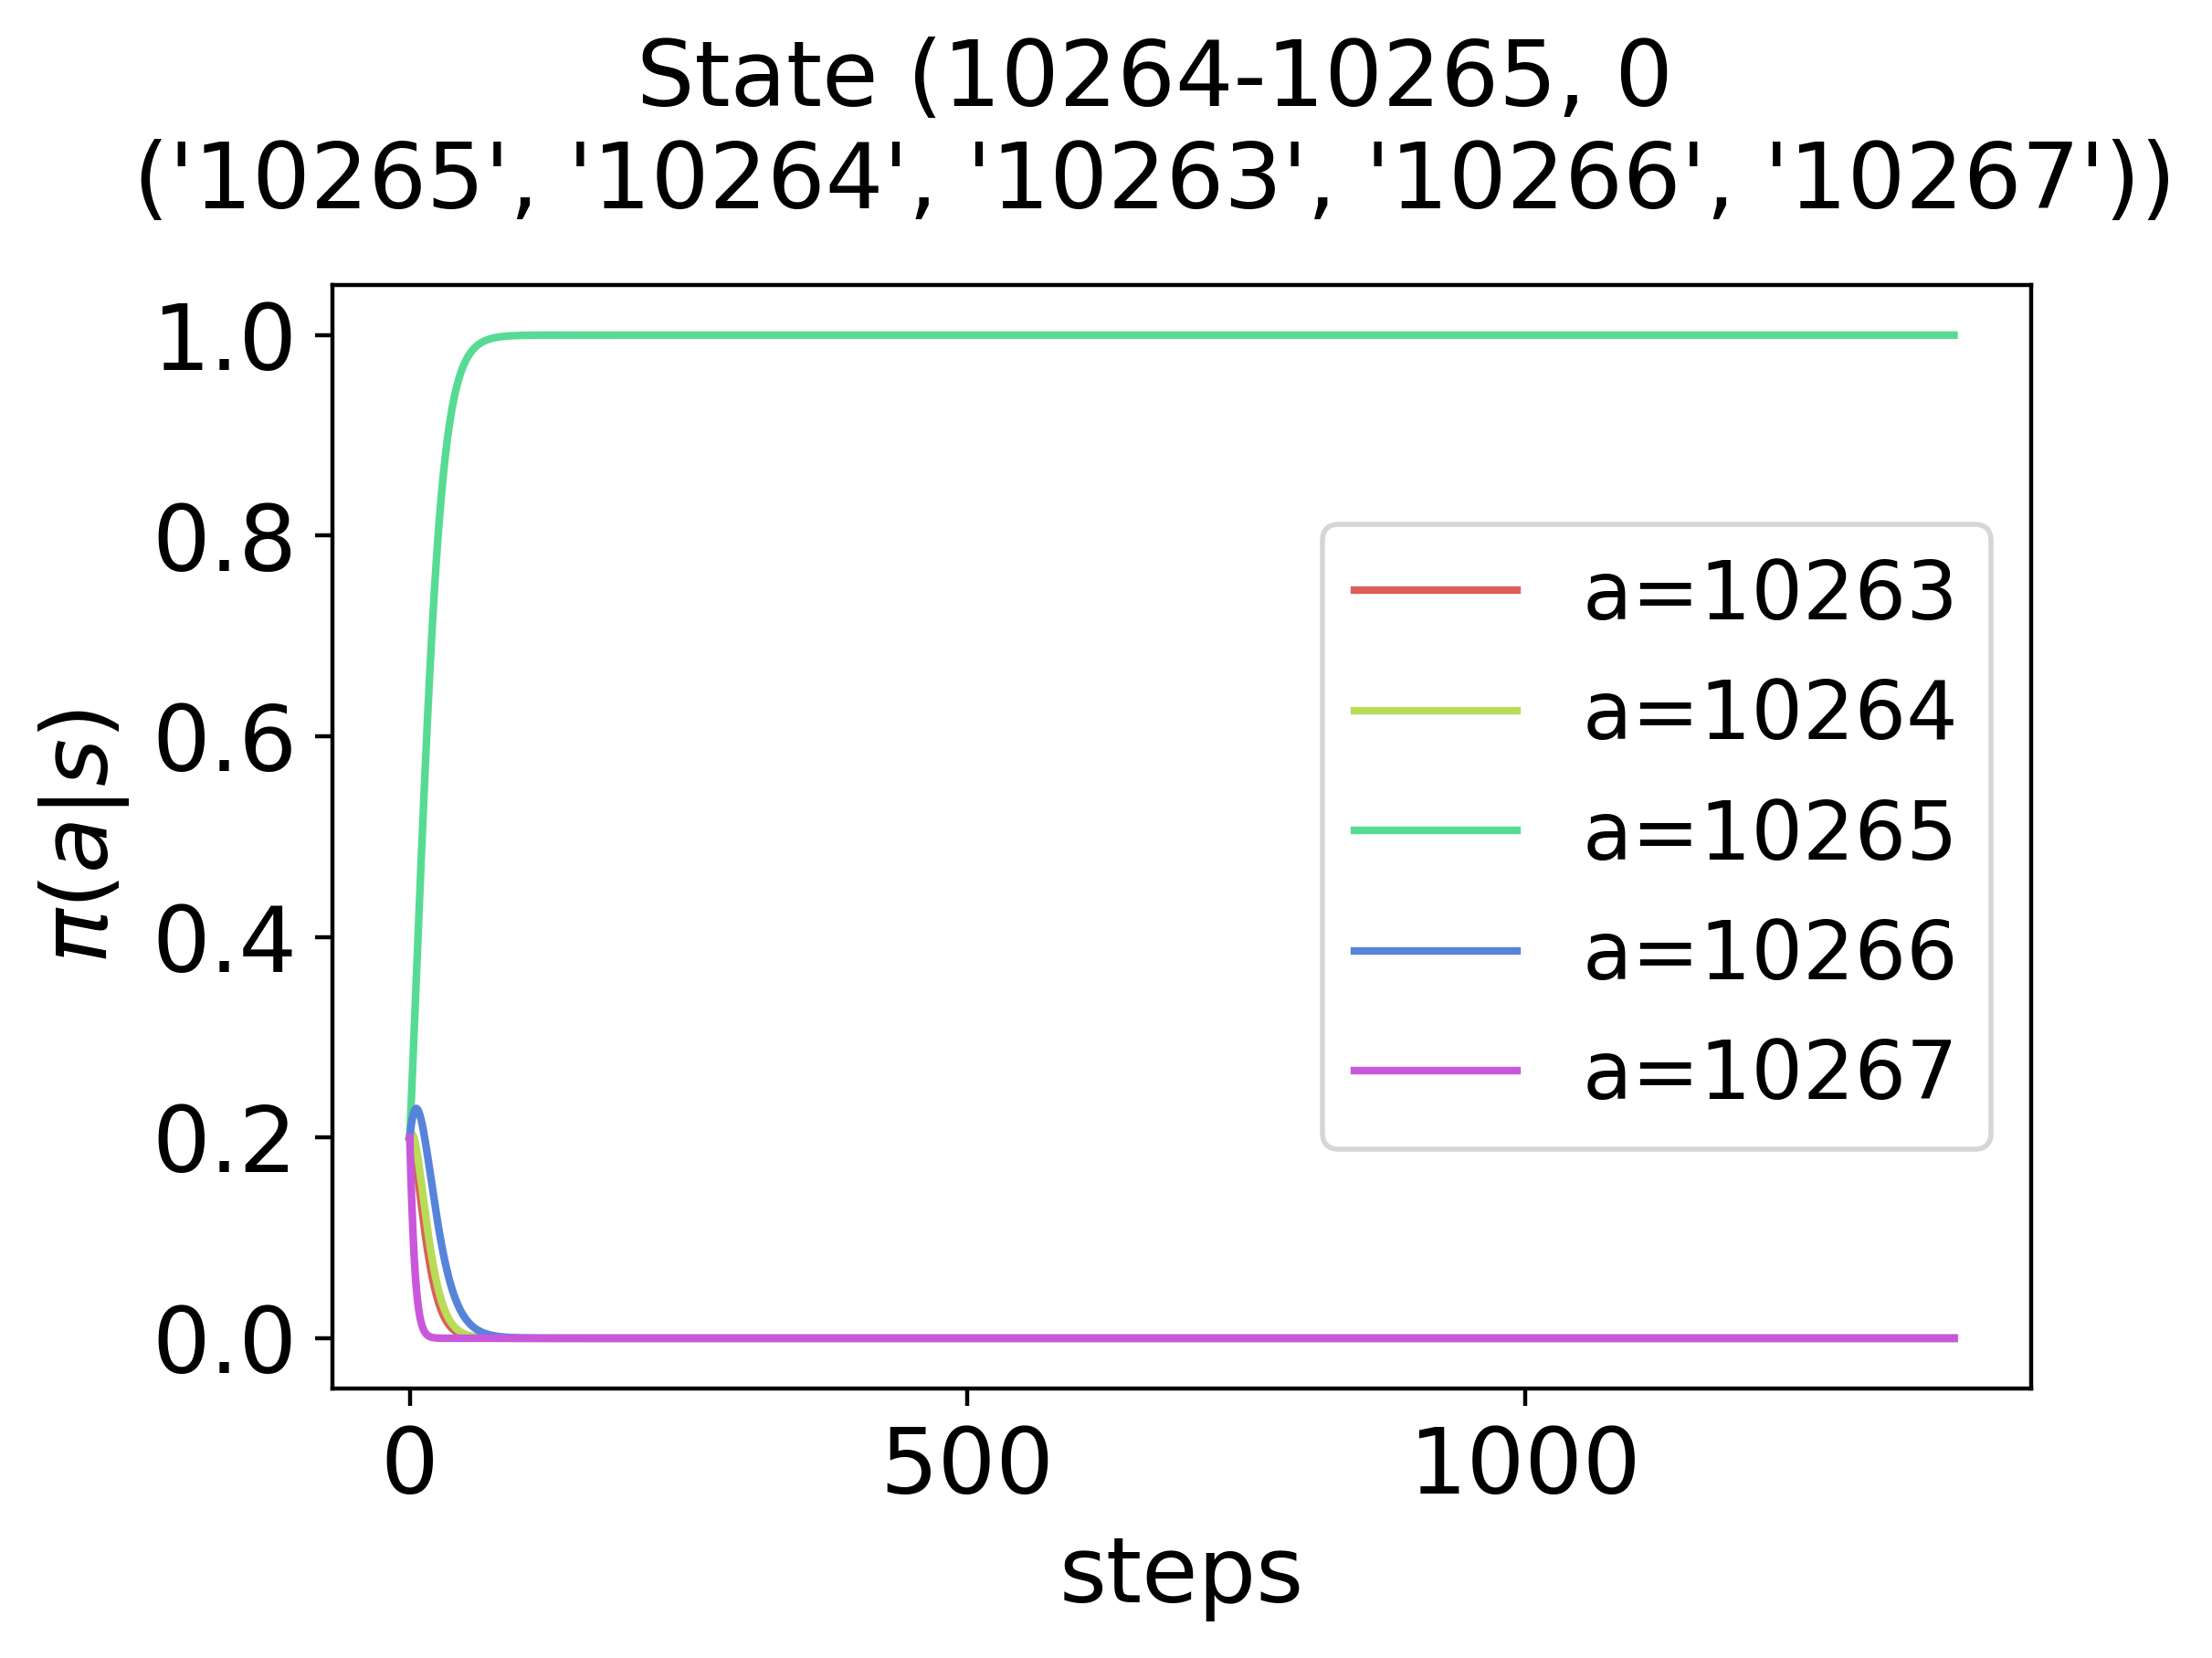
\includegraphics[scale=0.34,valign=b]{figures/policy_NPG_state_0.png} &
            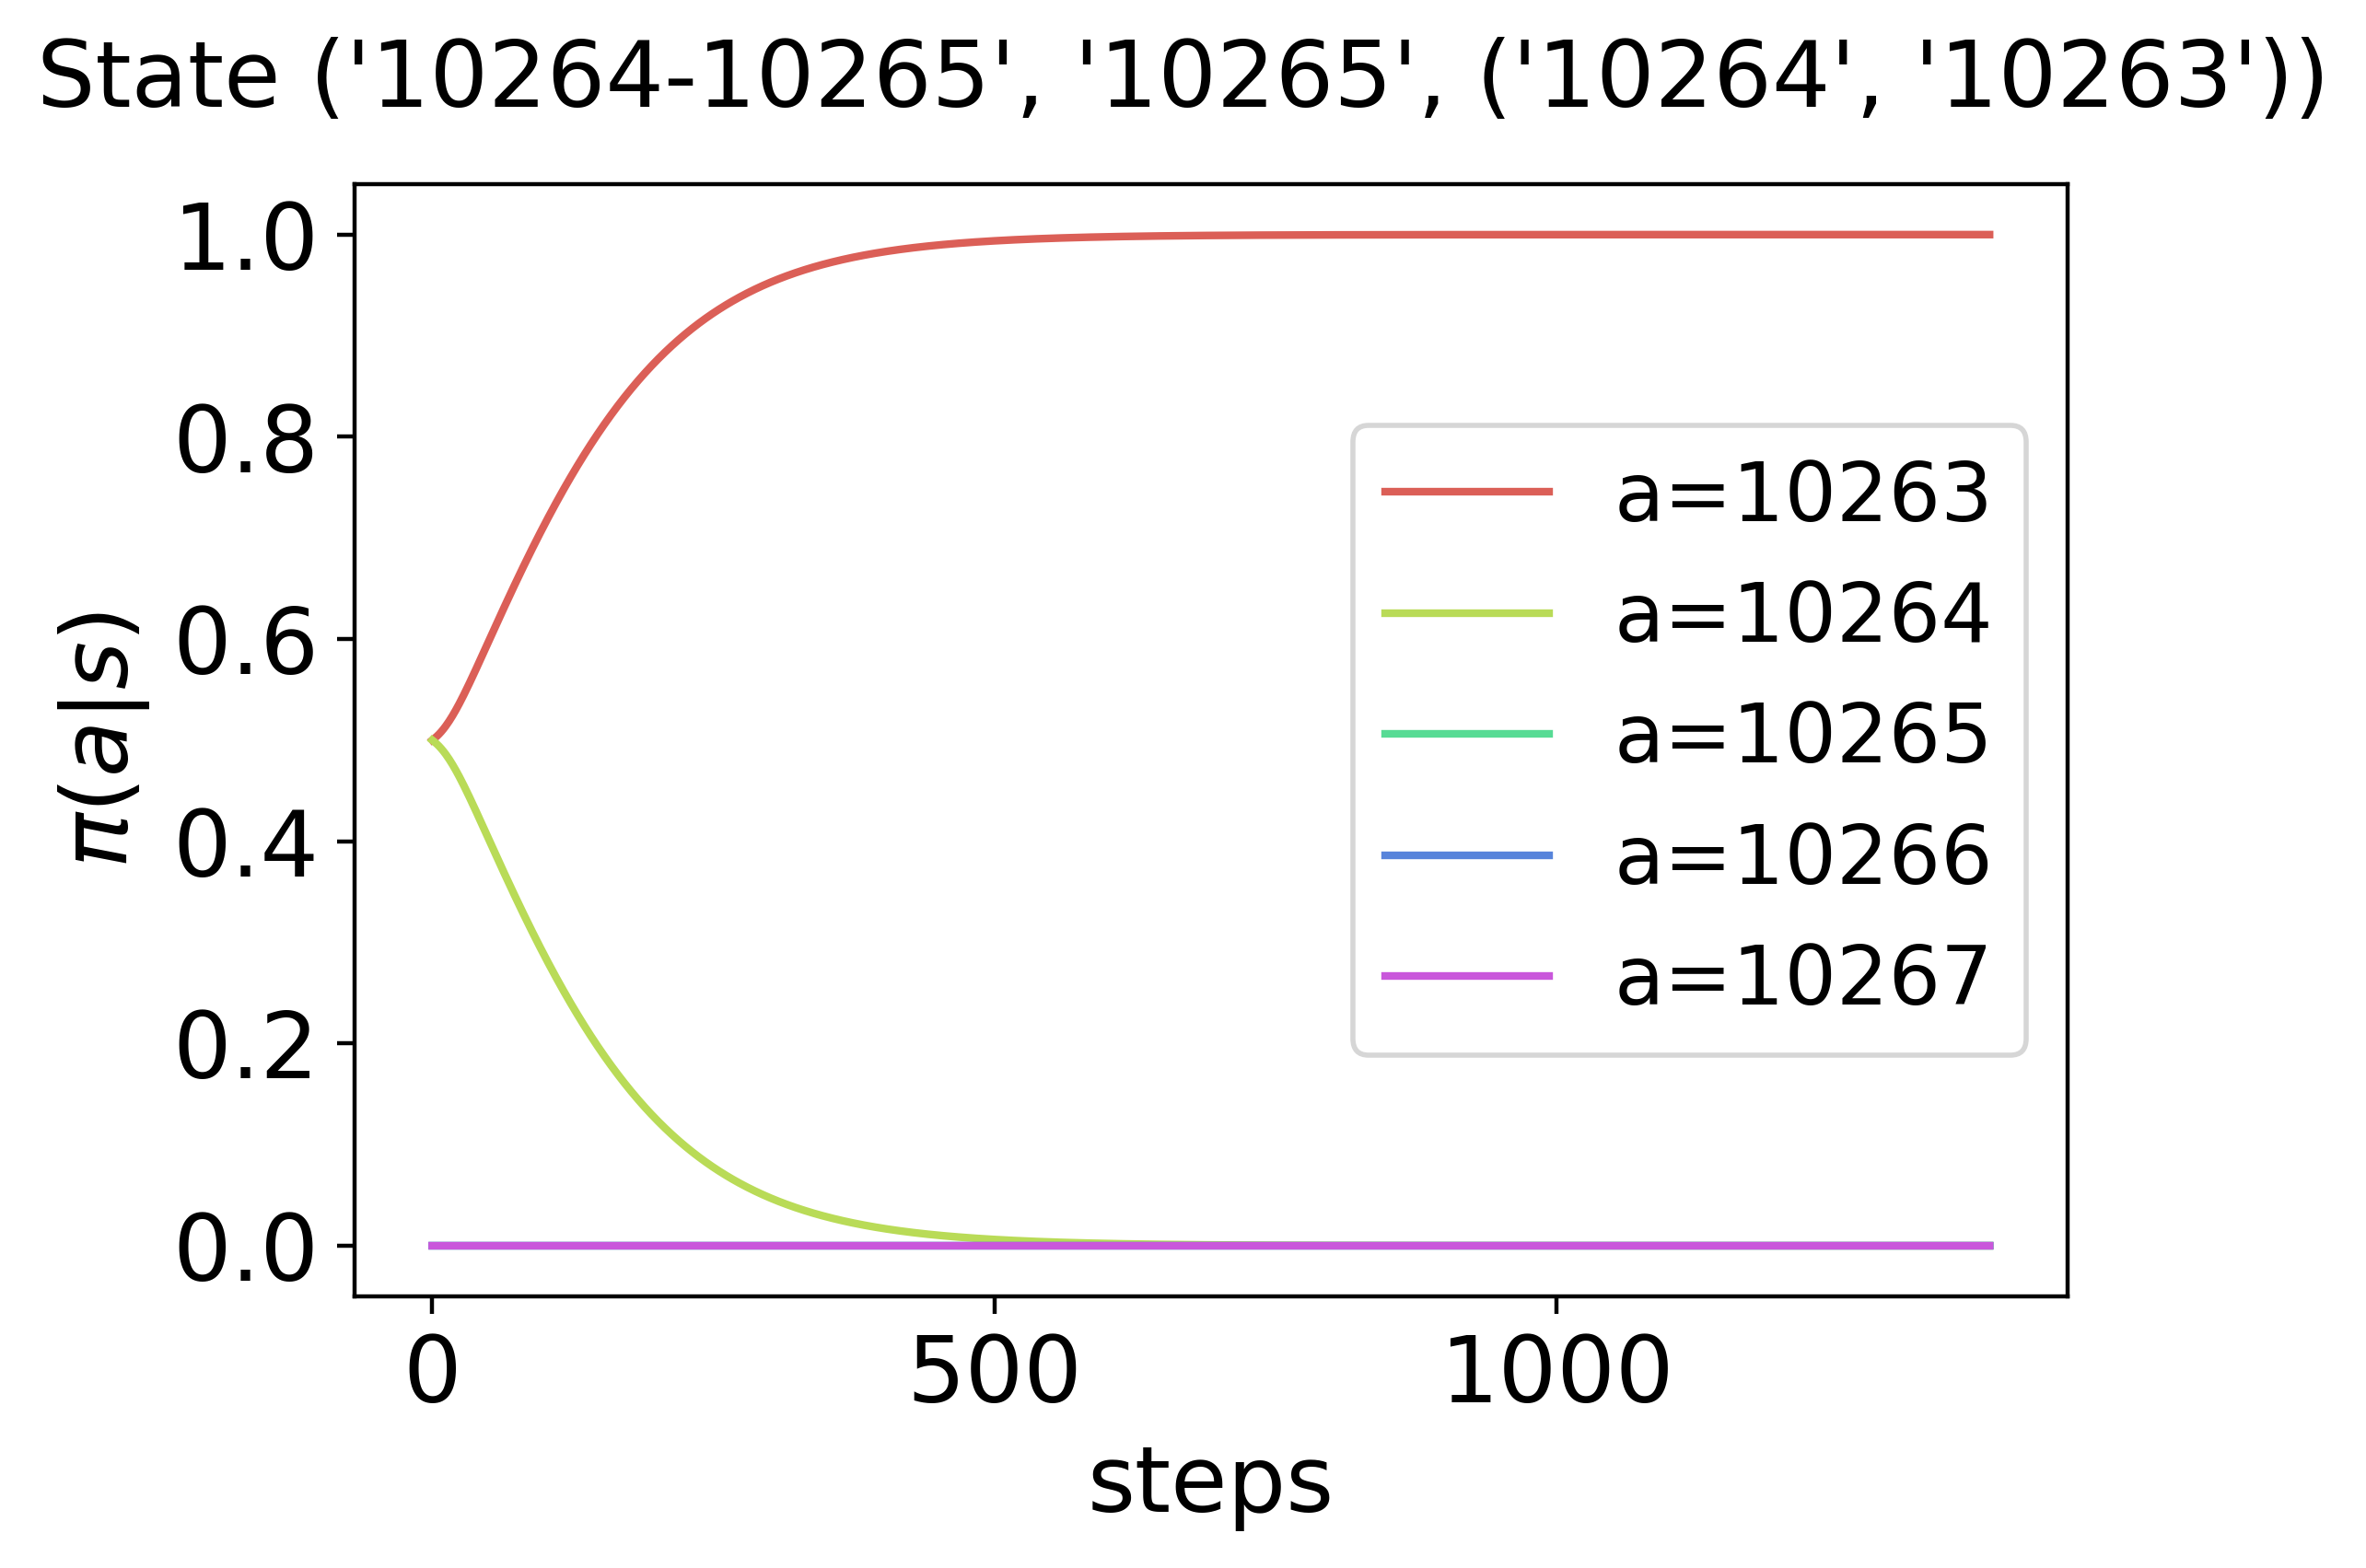
\includegraphics[scale=0.34,valign=b]{figures/policy_NPG_state_1.png} \\
            \hspace*{-5pt}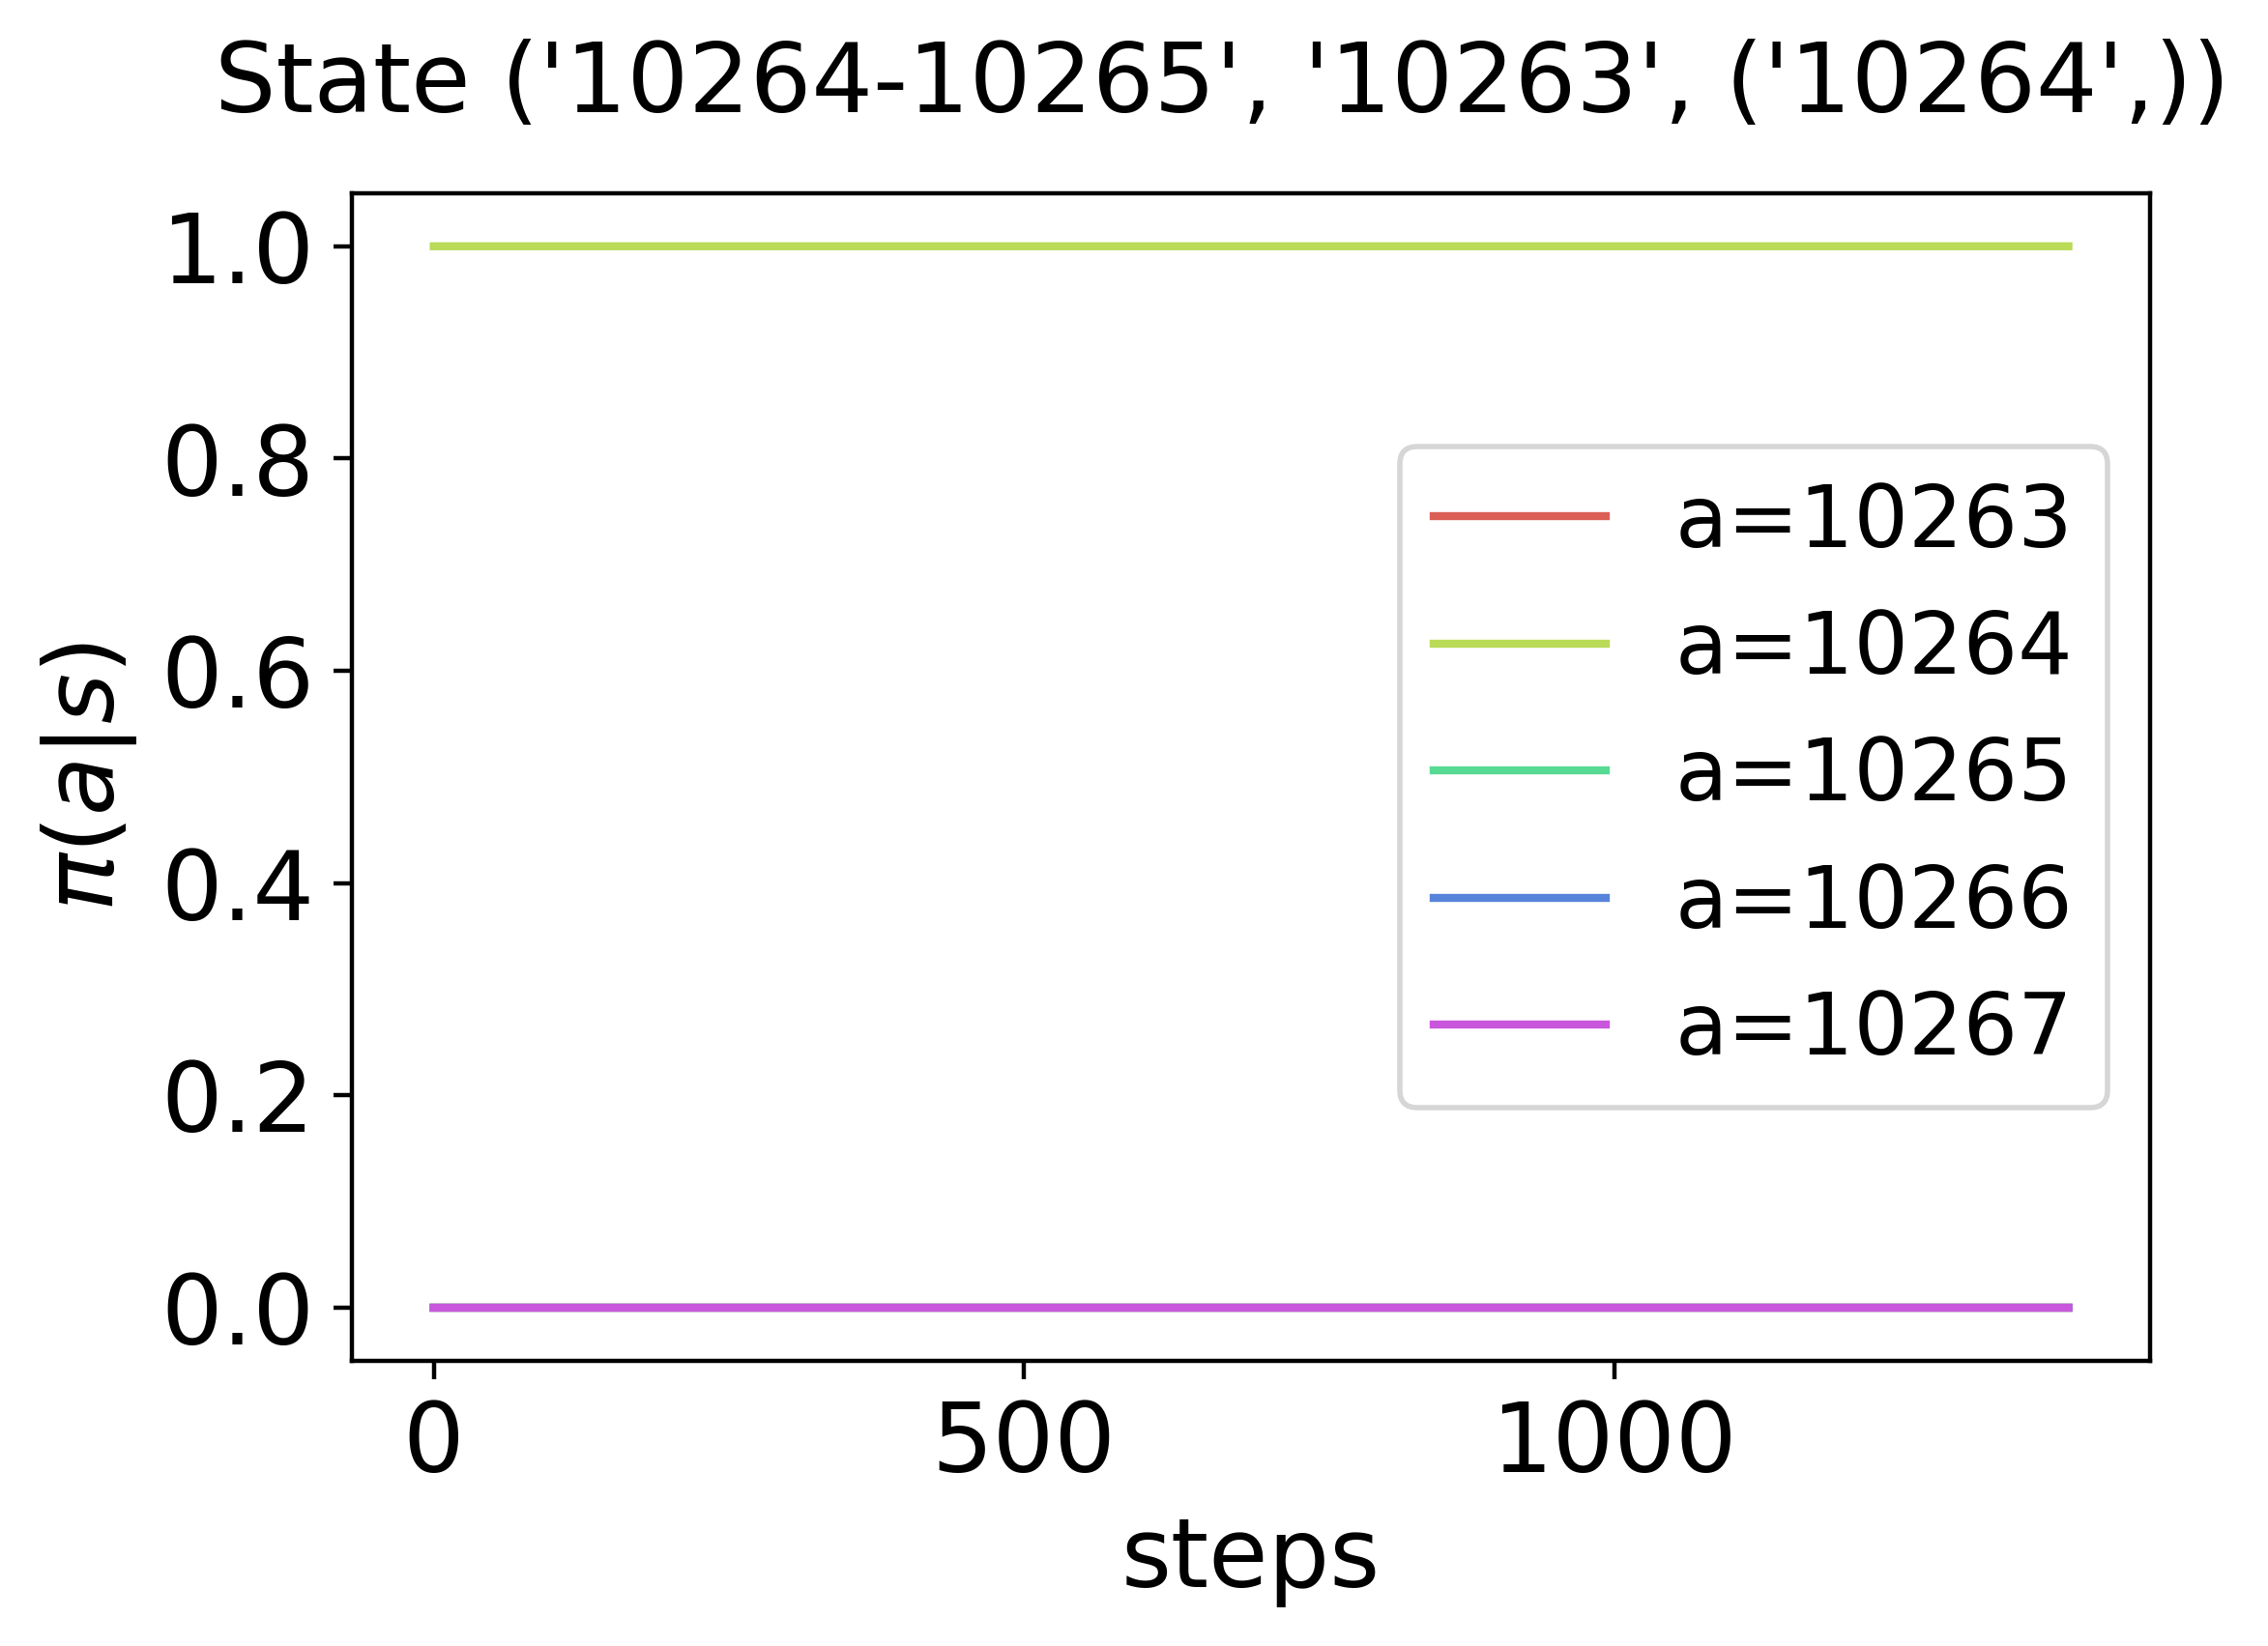
\includegraphics[scale=0.34,valign=b]{figures/policy_NPG_state_2.png} &
            \hspace*{-18pt}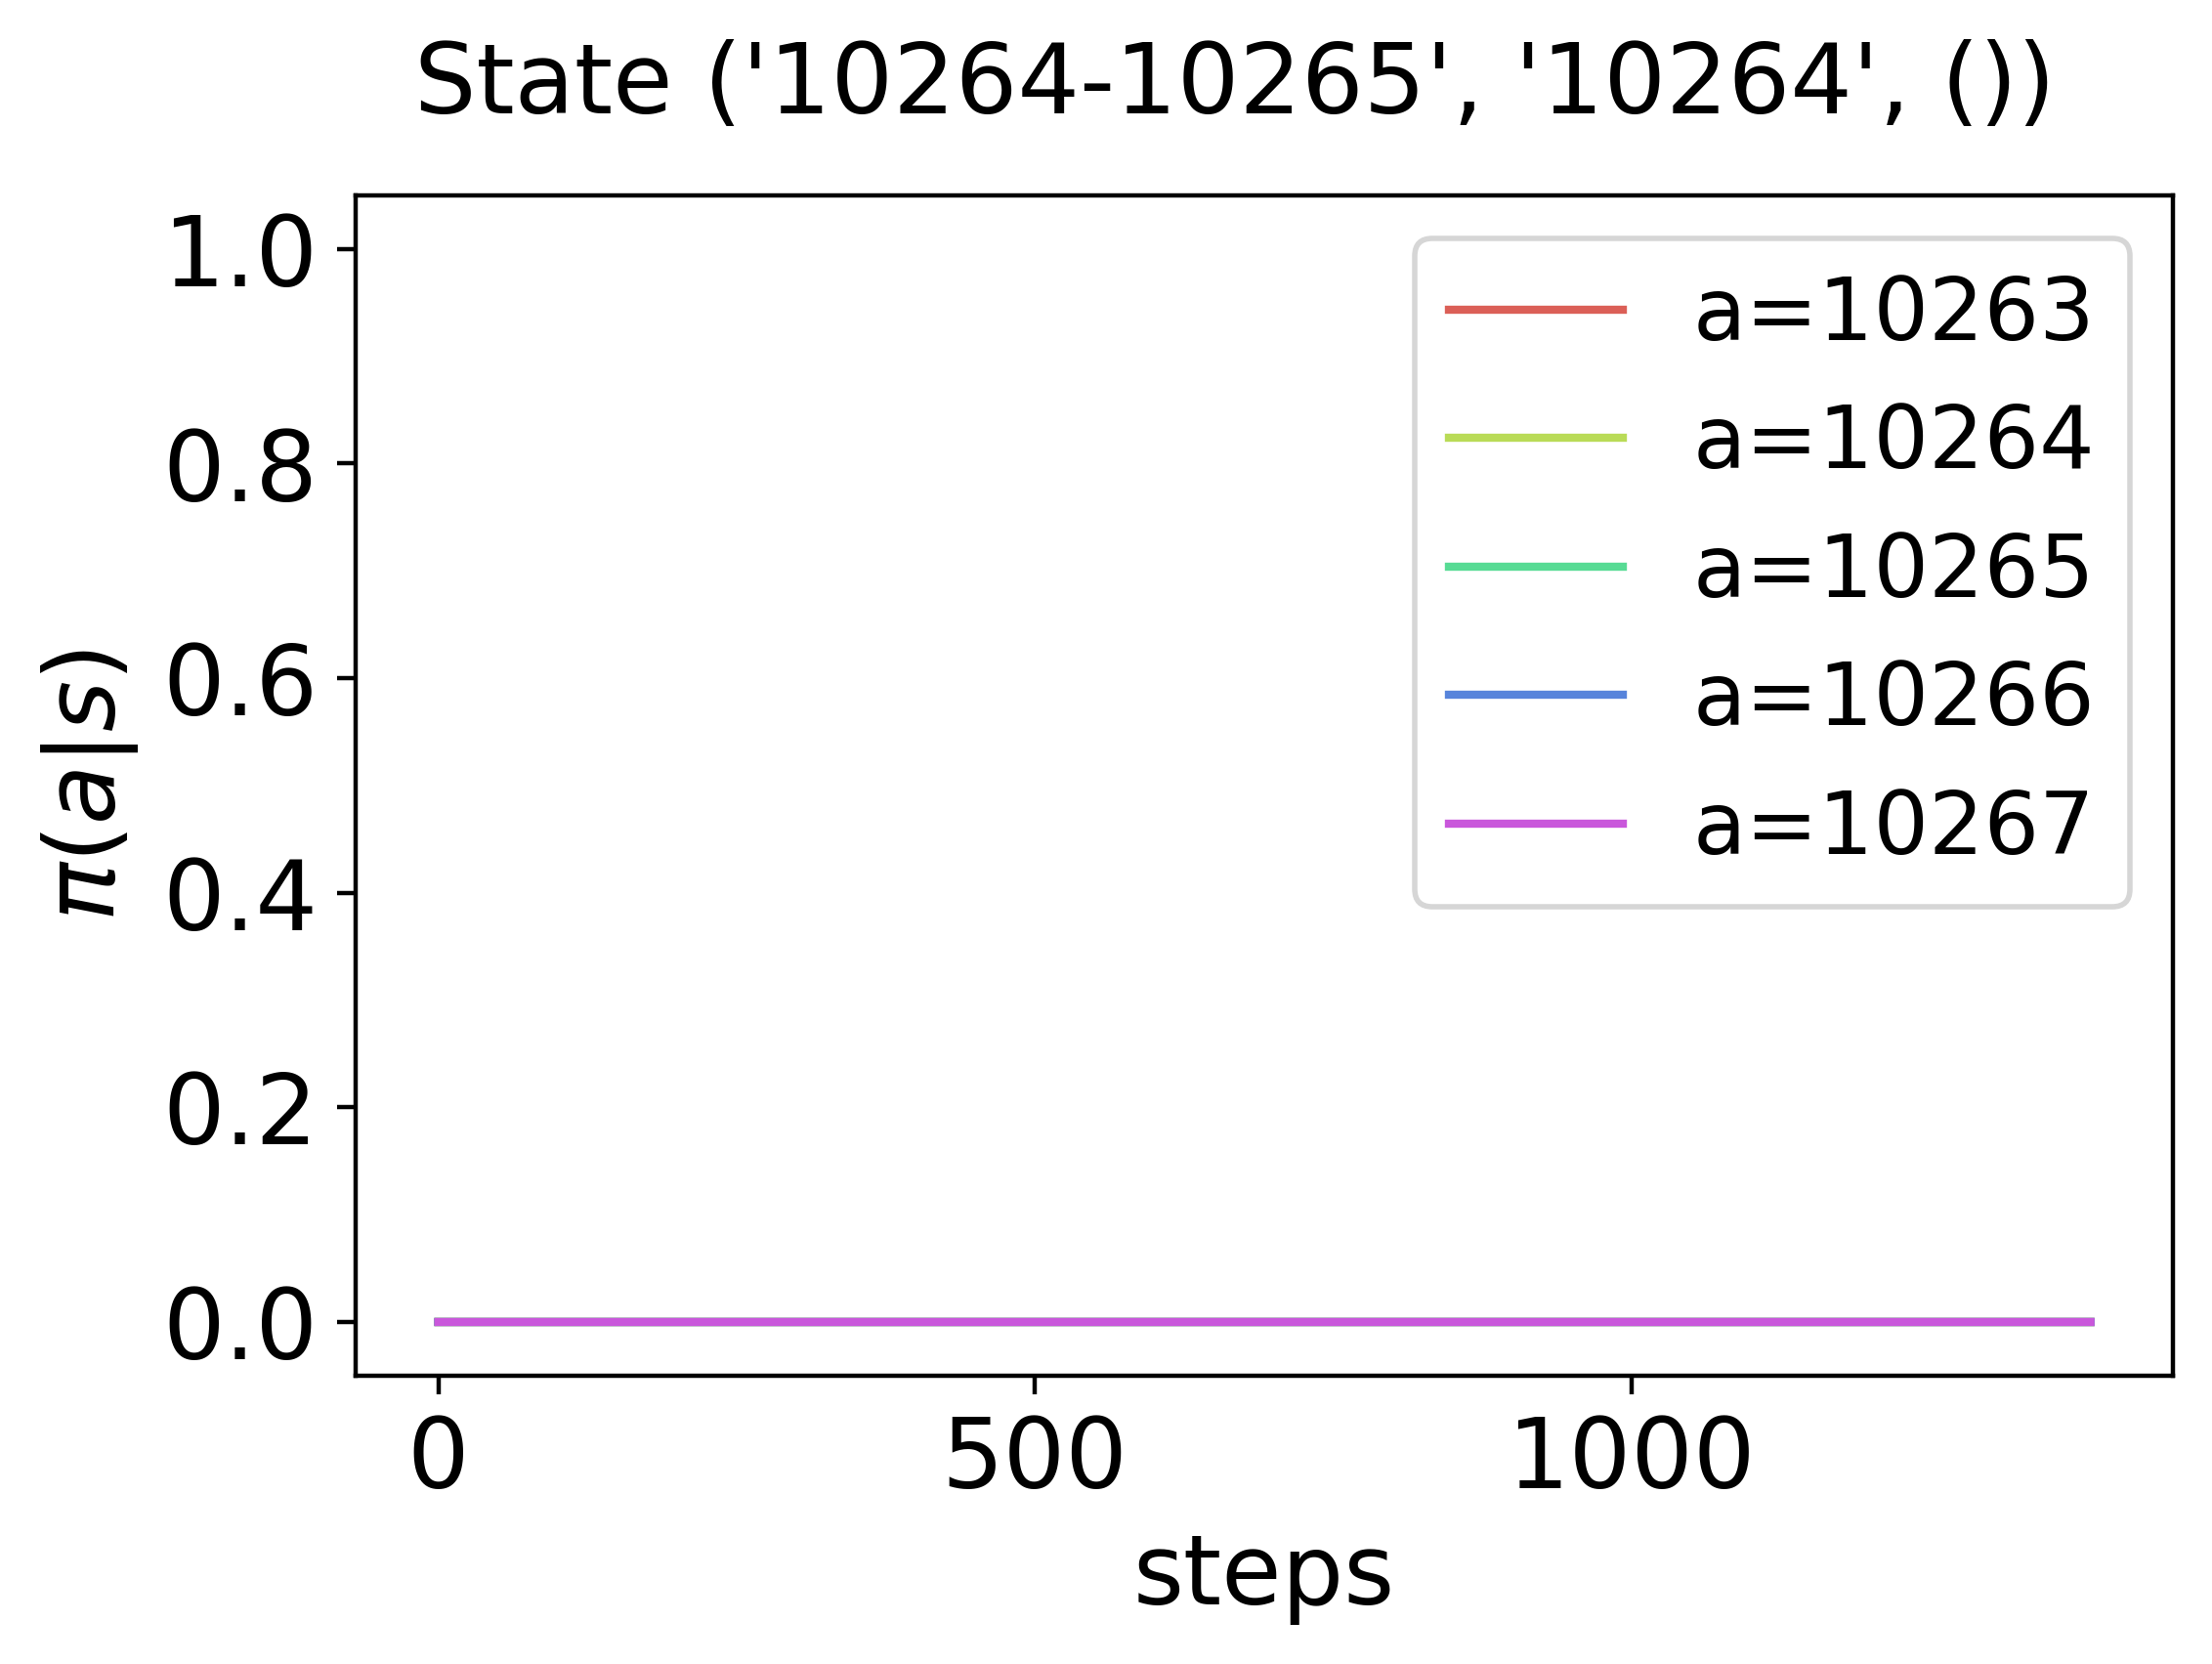
\includegraphics[scale=0.34,valign=b]{figures/policy_NPG_state_3.png}
        \end{tabular}
    \end{figure}
    
\end{frame}

\begin{frame}{}

    \begin{figure}
        \centering
        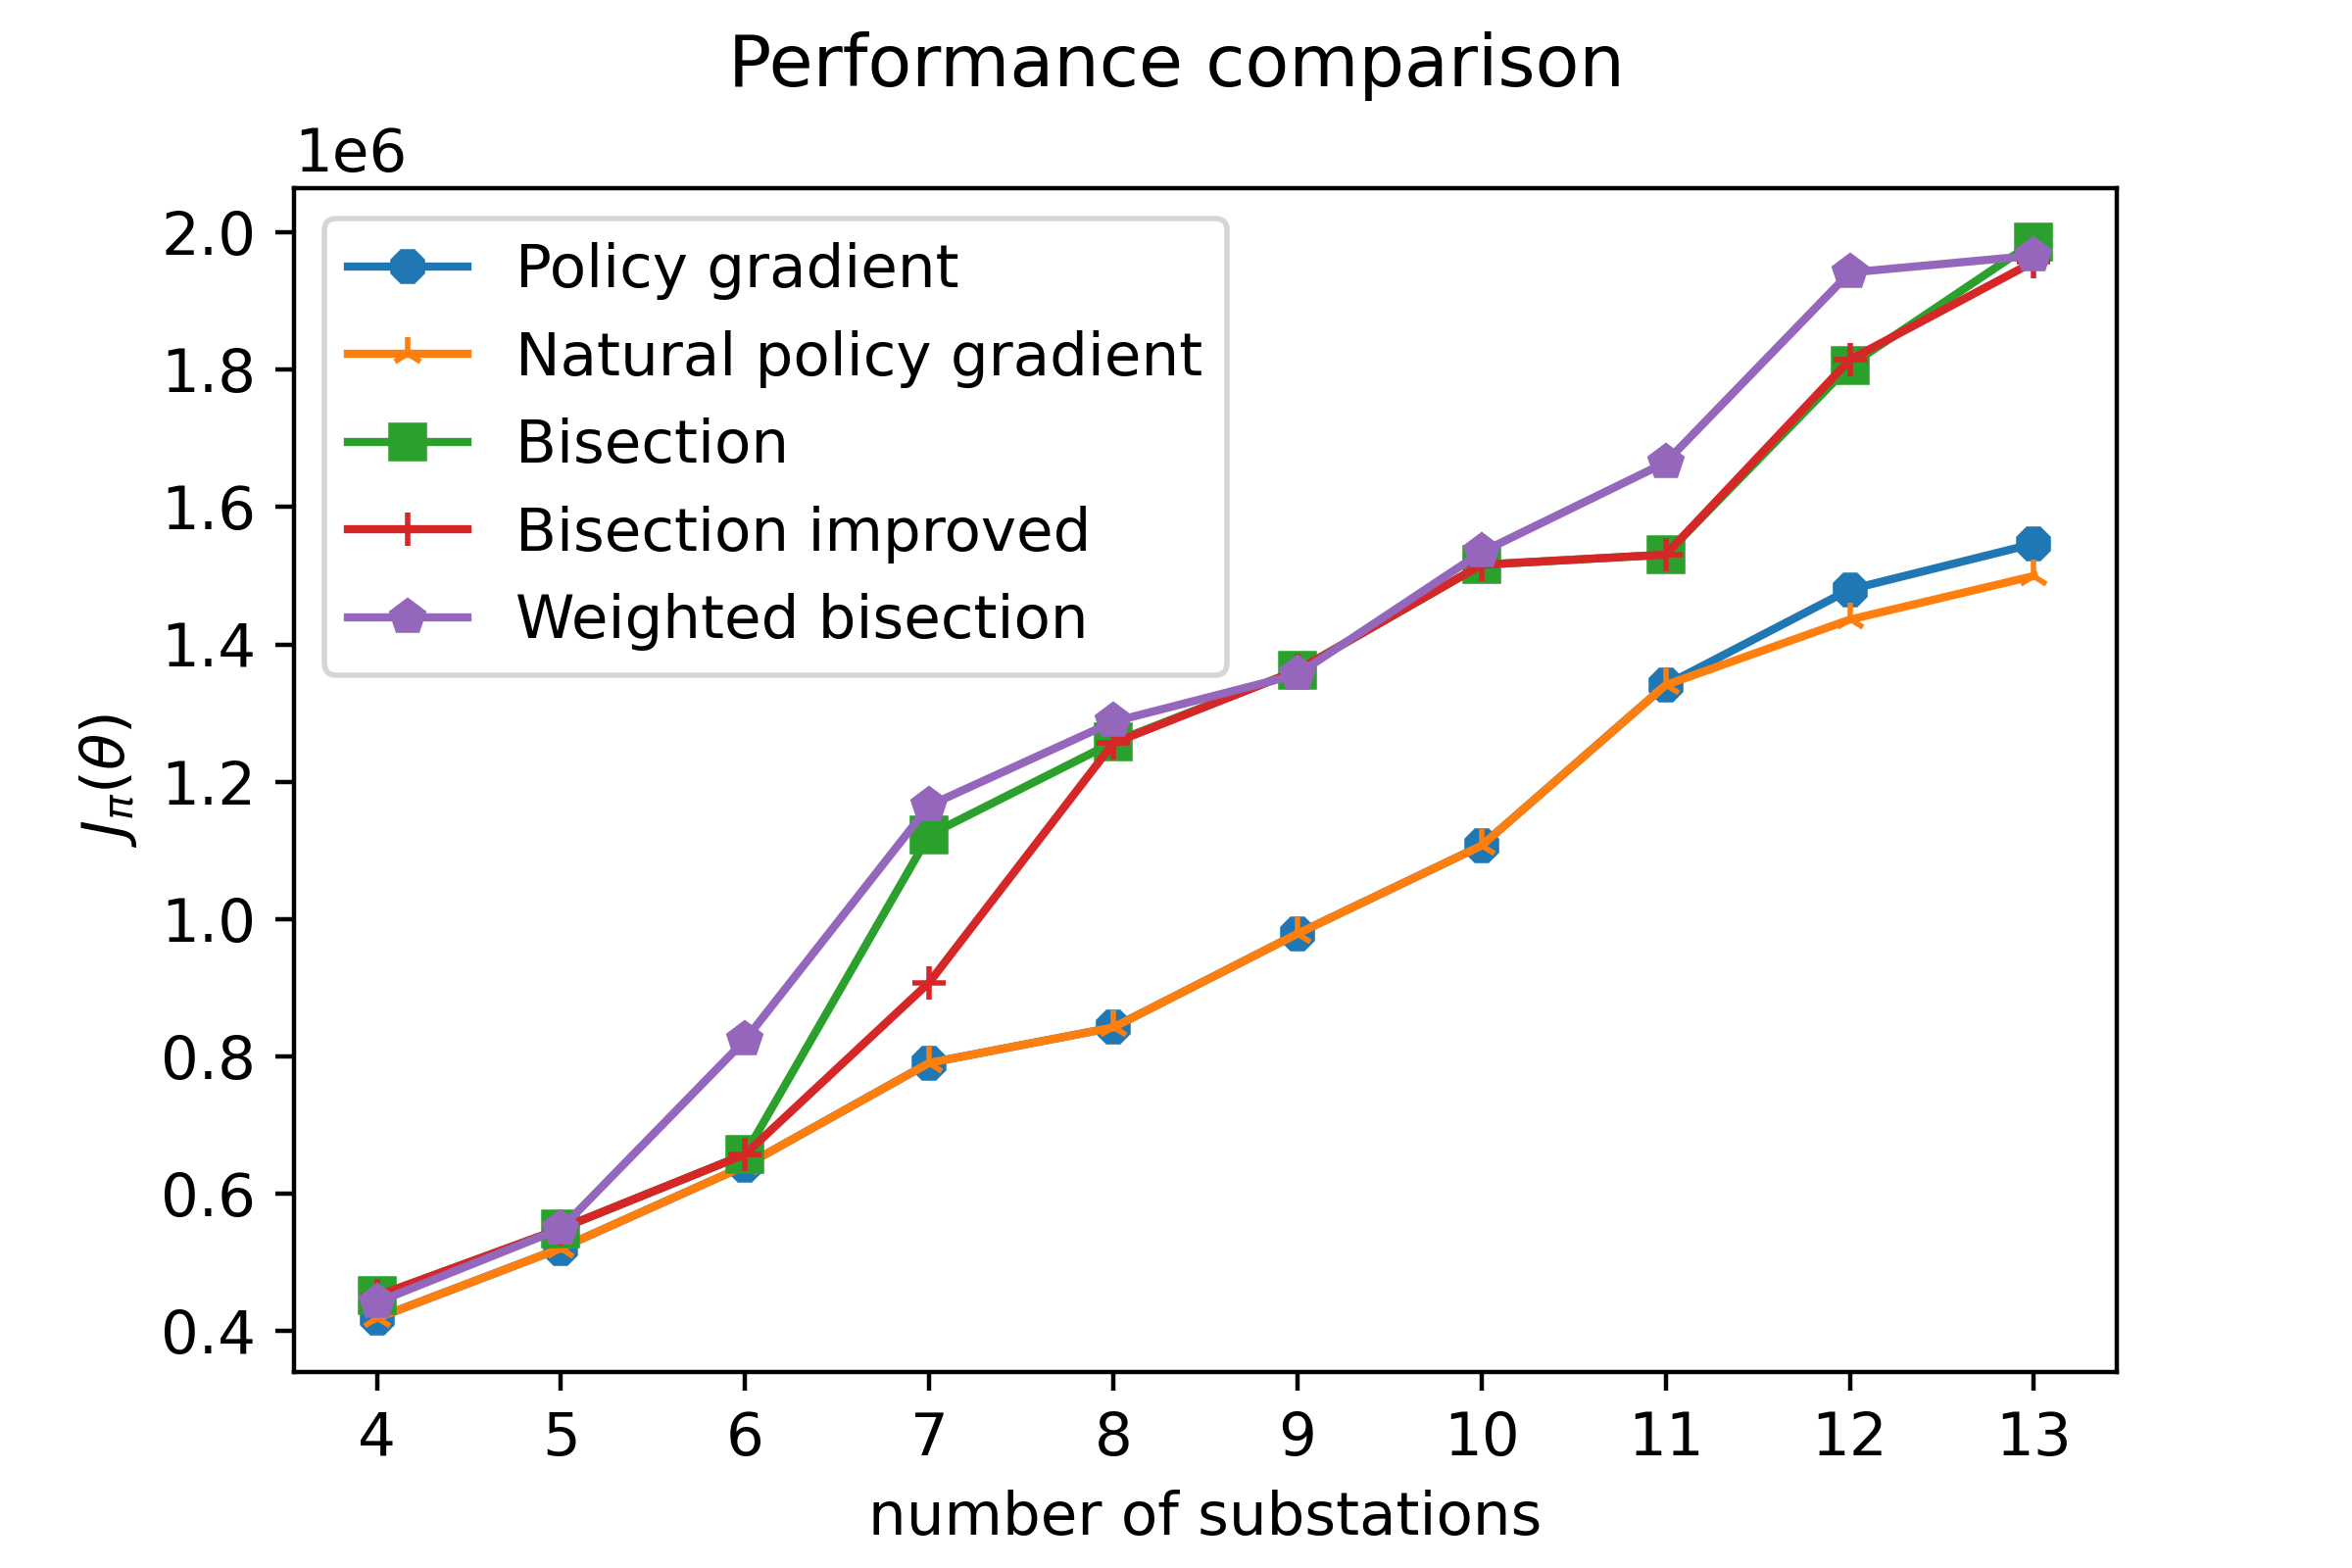
\includegraphics[scale=0.85]{figures/comparison_graph.png}
    \end{figure}
    
\end{frame}

{\putbgdark
\begin{frame}[standout]
	\begin{center}
		\Large \uncover<+->{Thank you for your attention!}
		
		\Huge\uncover<+->{\Smiley}
	\end{center}
\end{frame}
}

{\putbg
\section{Backup slides}
}

\begin{frame}{}

    \begin{figure}
        \centering
        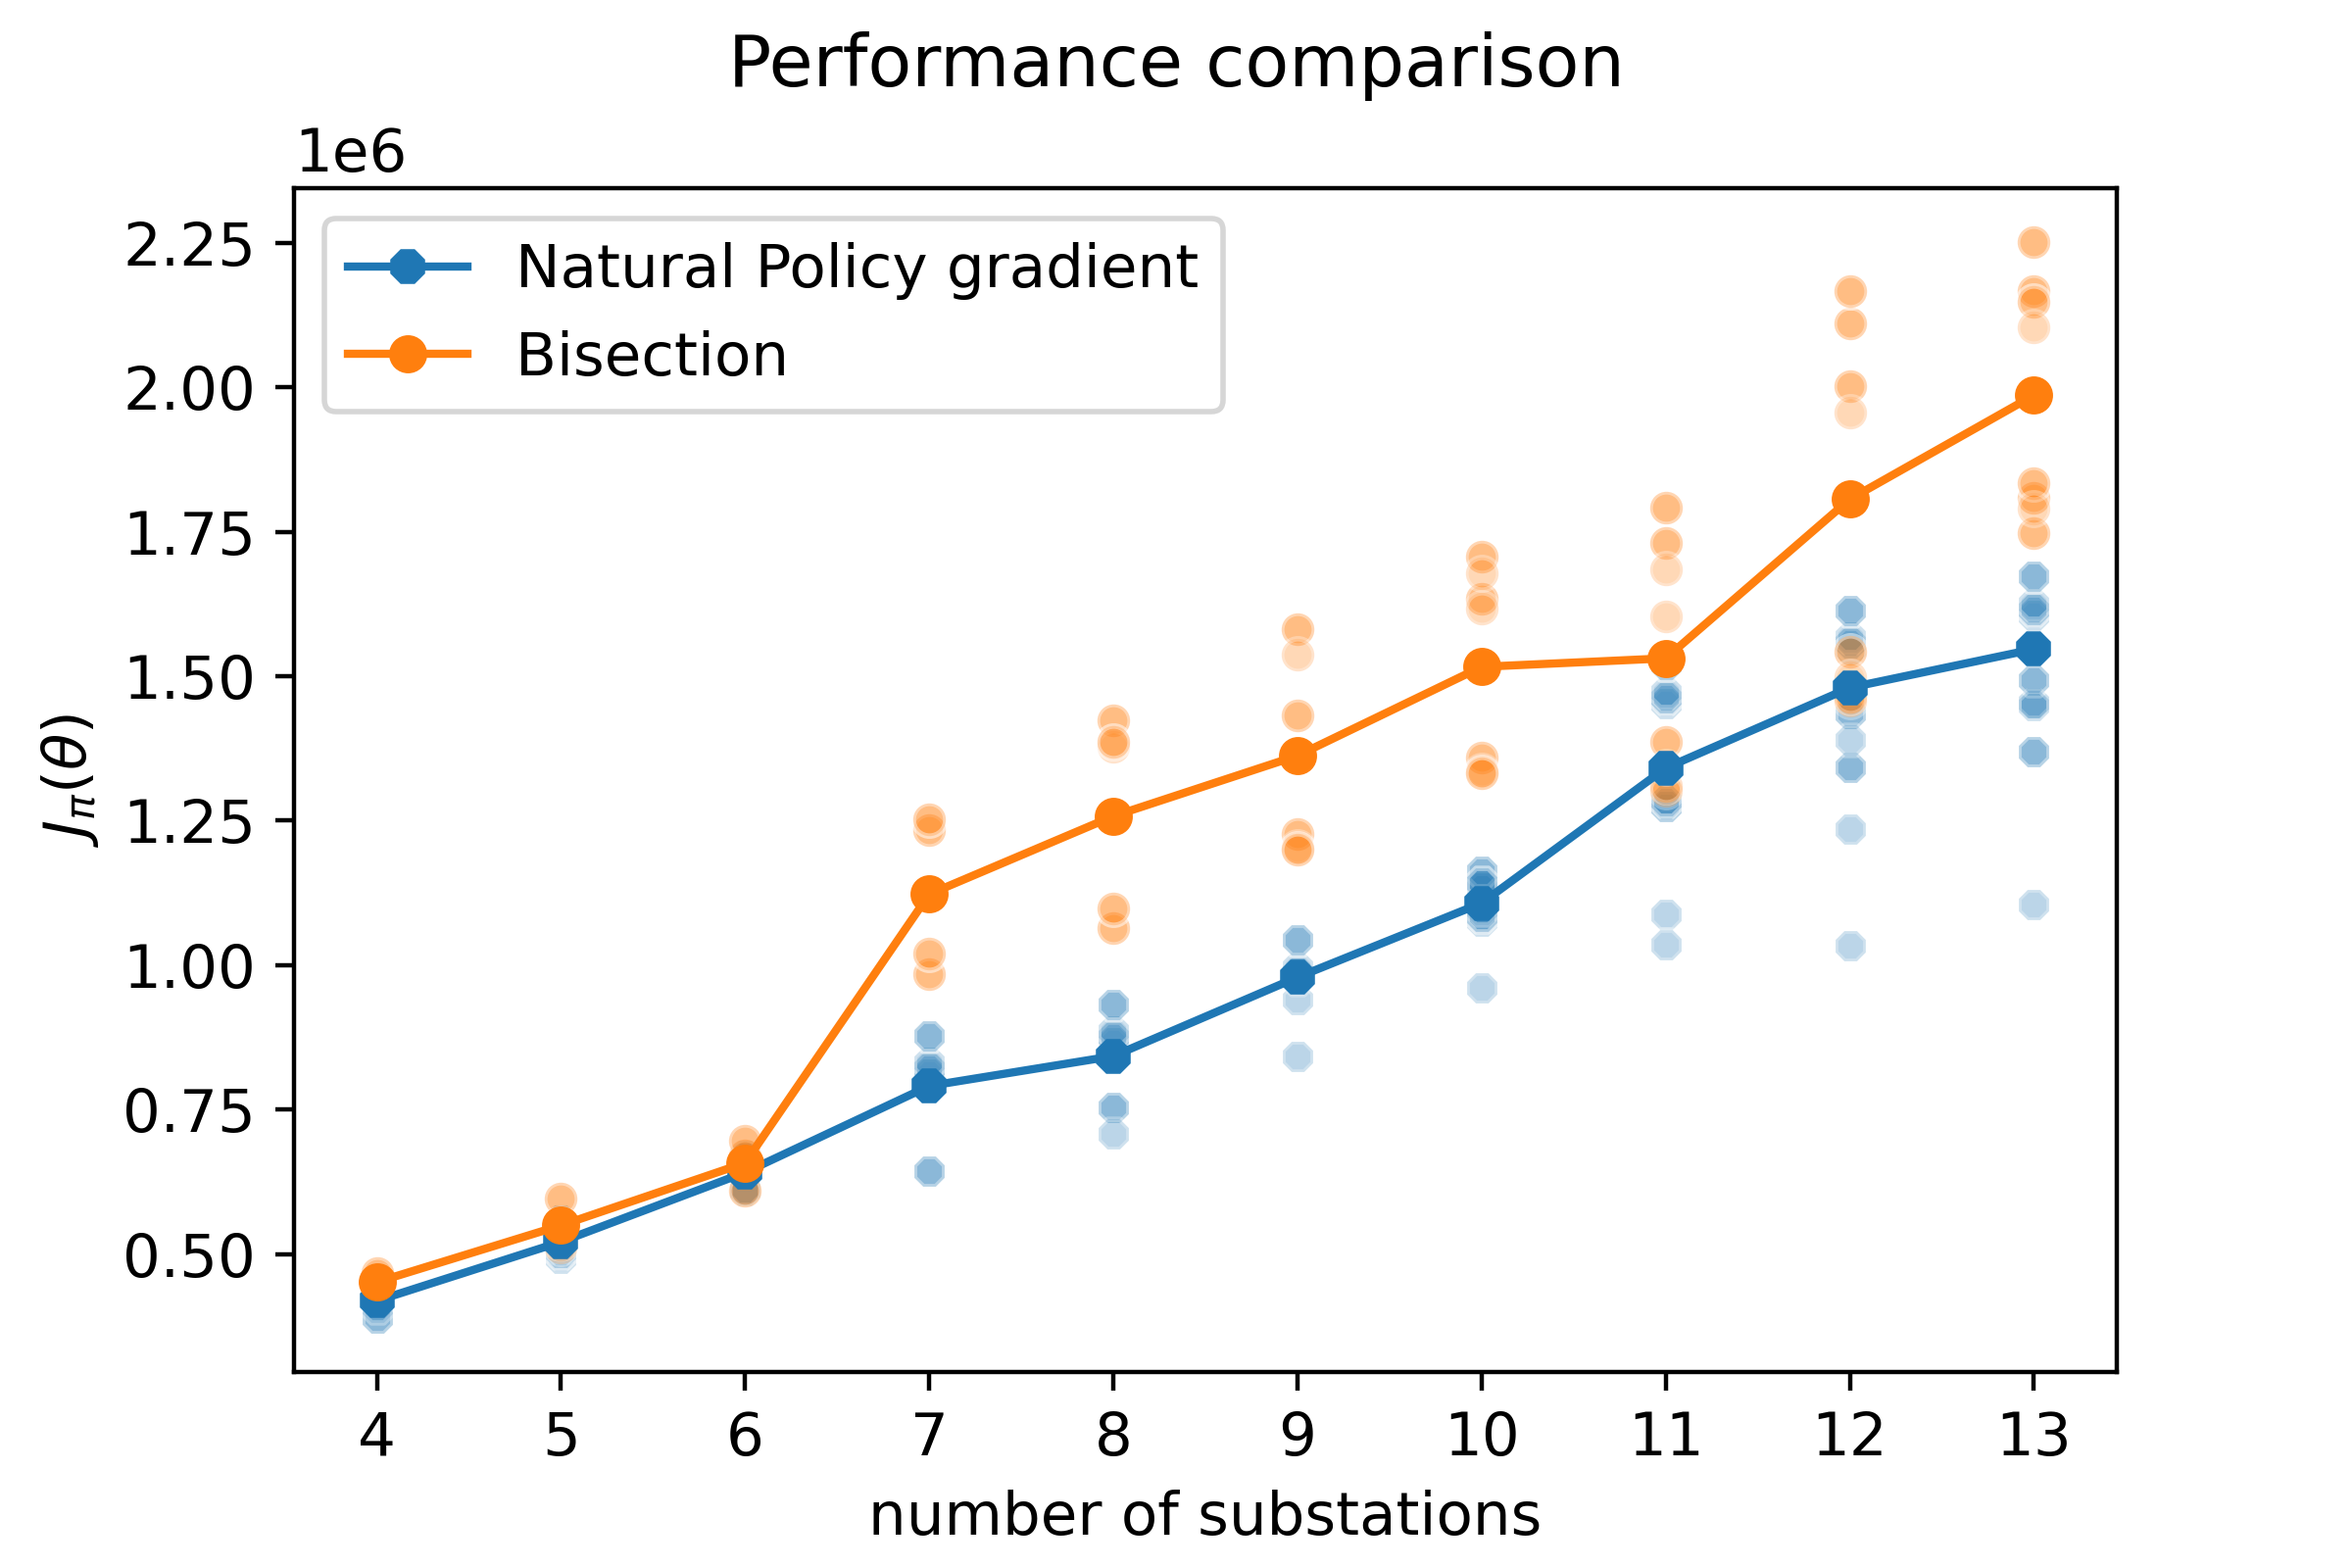
\includegraphics[scale=0.85]{figures/comparison_graph_scatterplot.png}
    \end{figure}
    
\end{frame}

\begin{frame}{}

    \begin{figure}
        \centering
        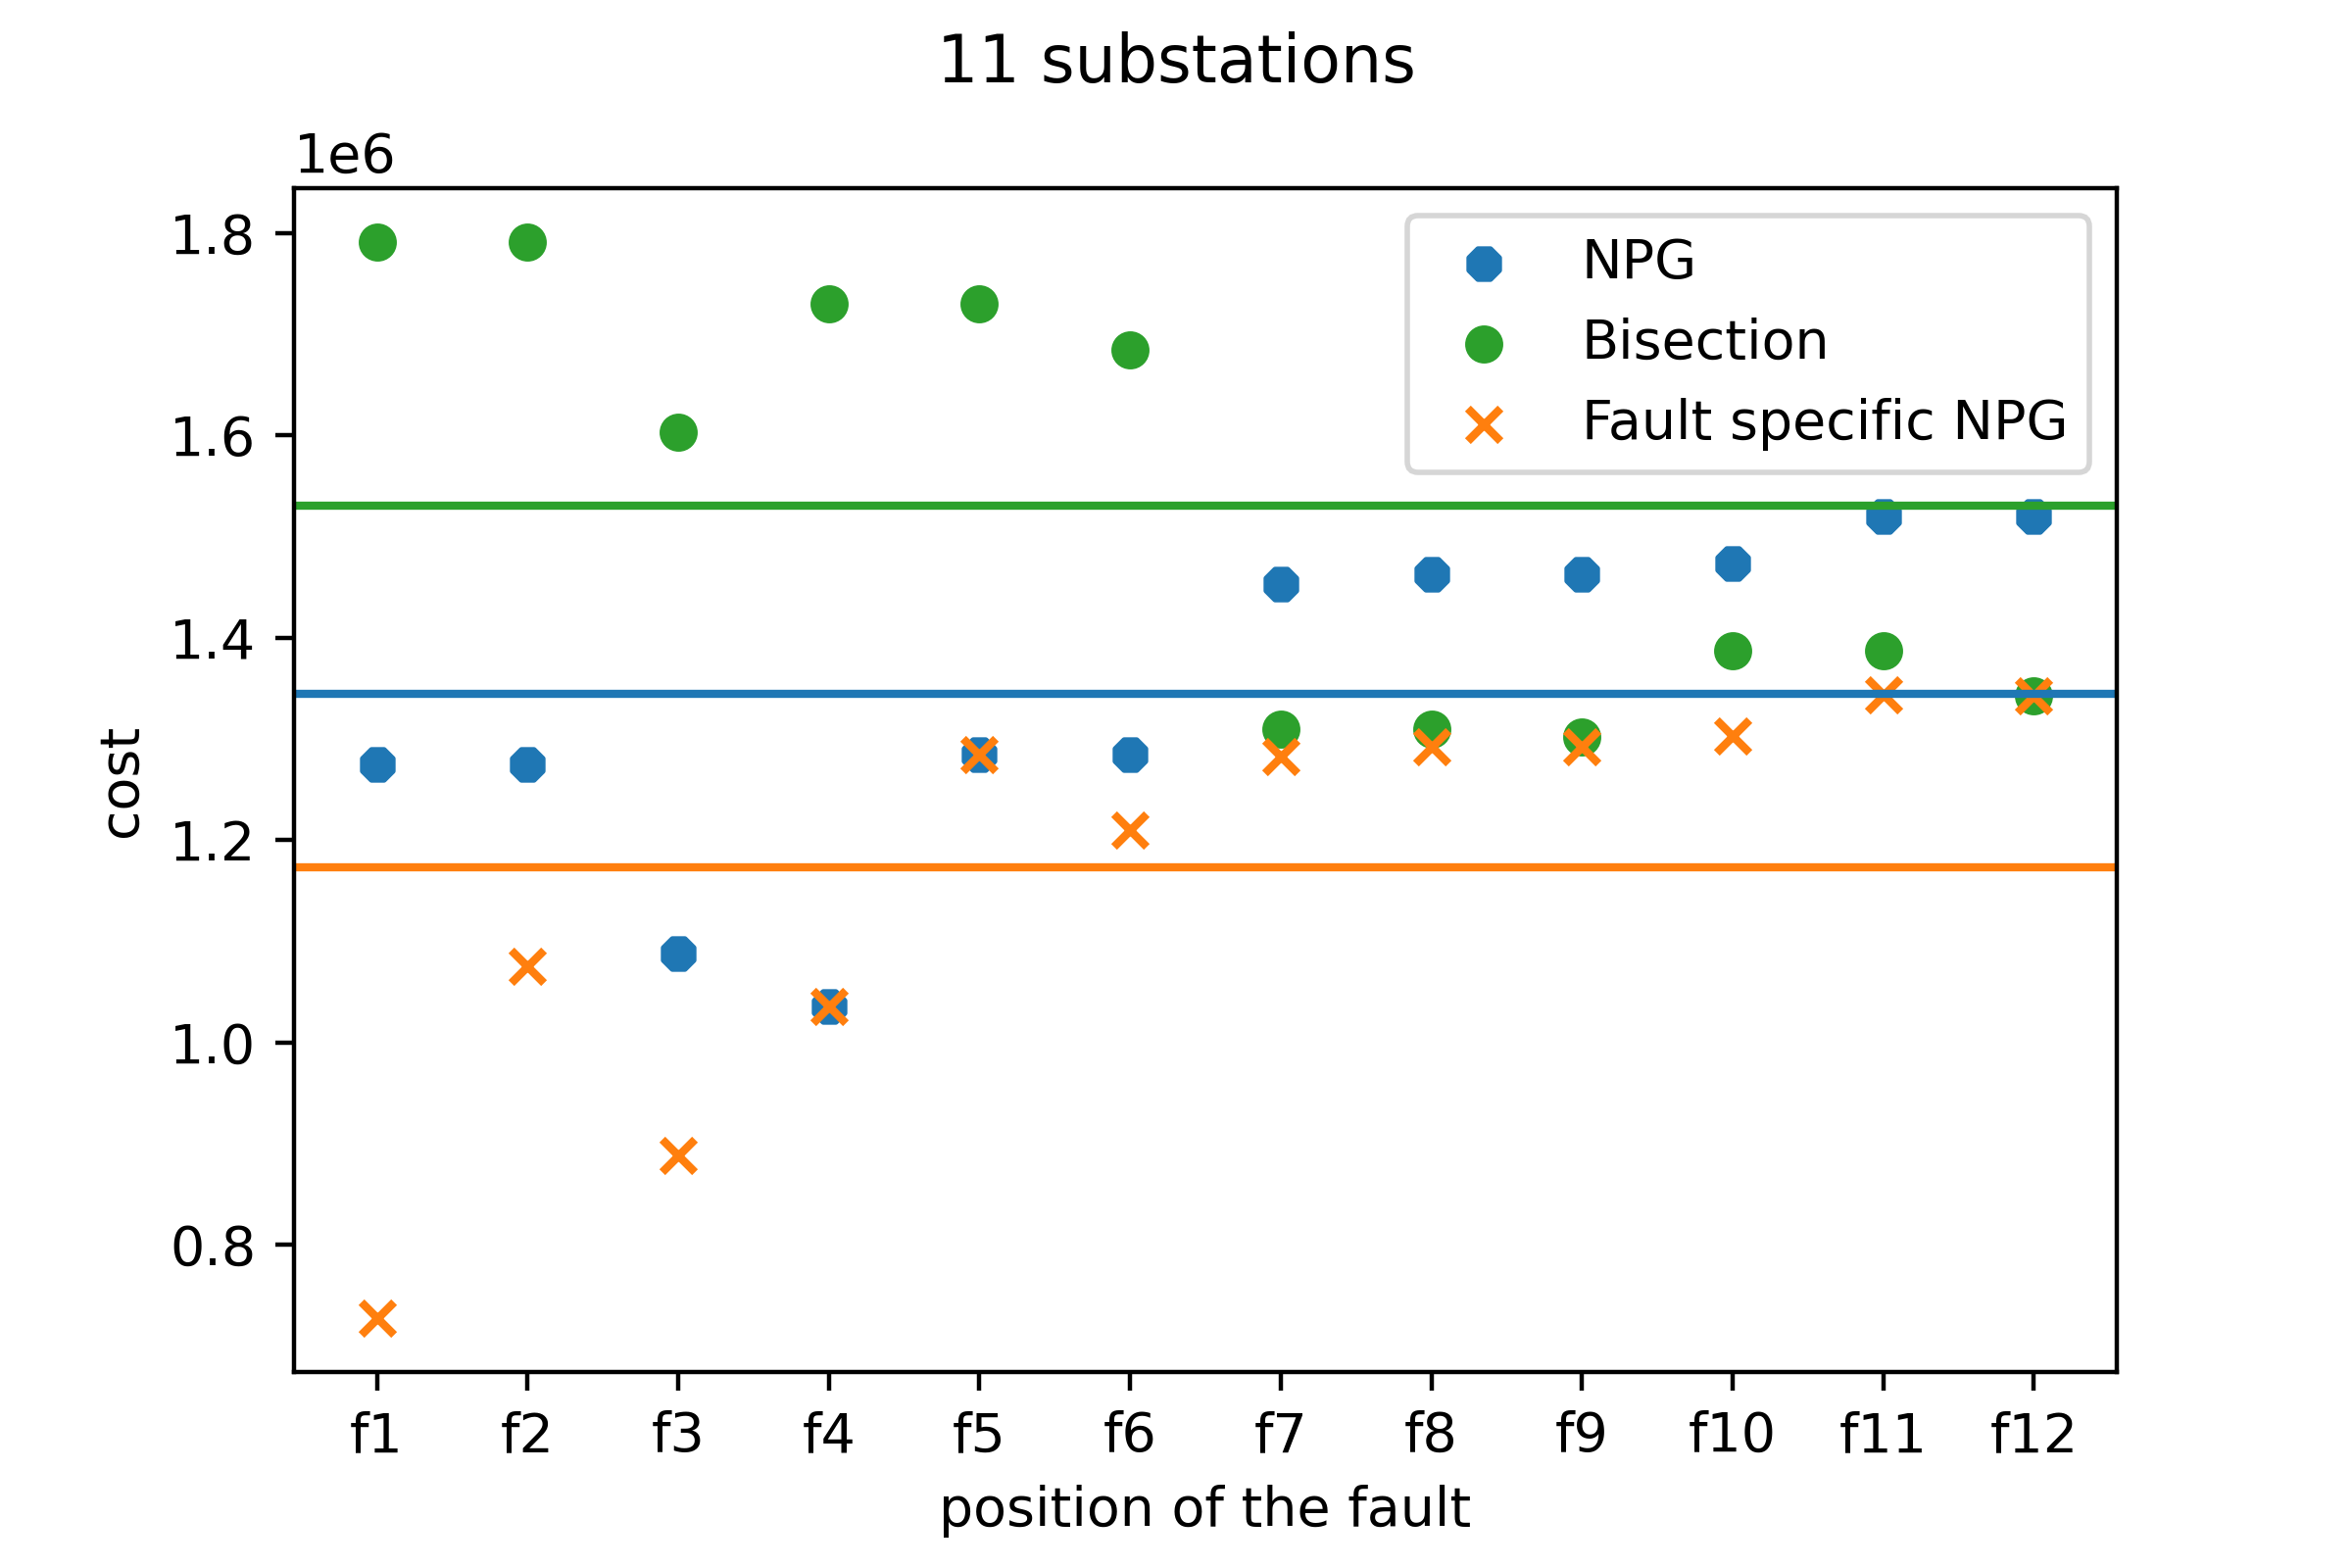
\includegraphics[scale=0.85]{figures/scatterplot.png}
    \end{figure}
    
\end{frame}

\begin{frame}{}

    \vspace*{-10pt}
    \begin{figure}
        \centering
        \hspace*{-13pt}
        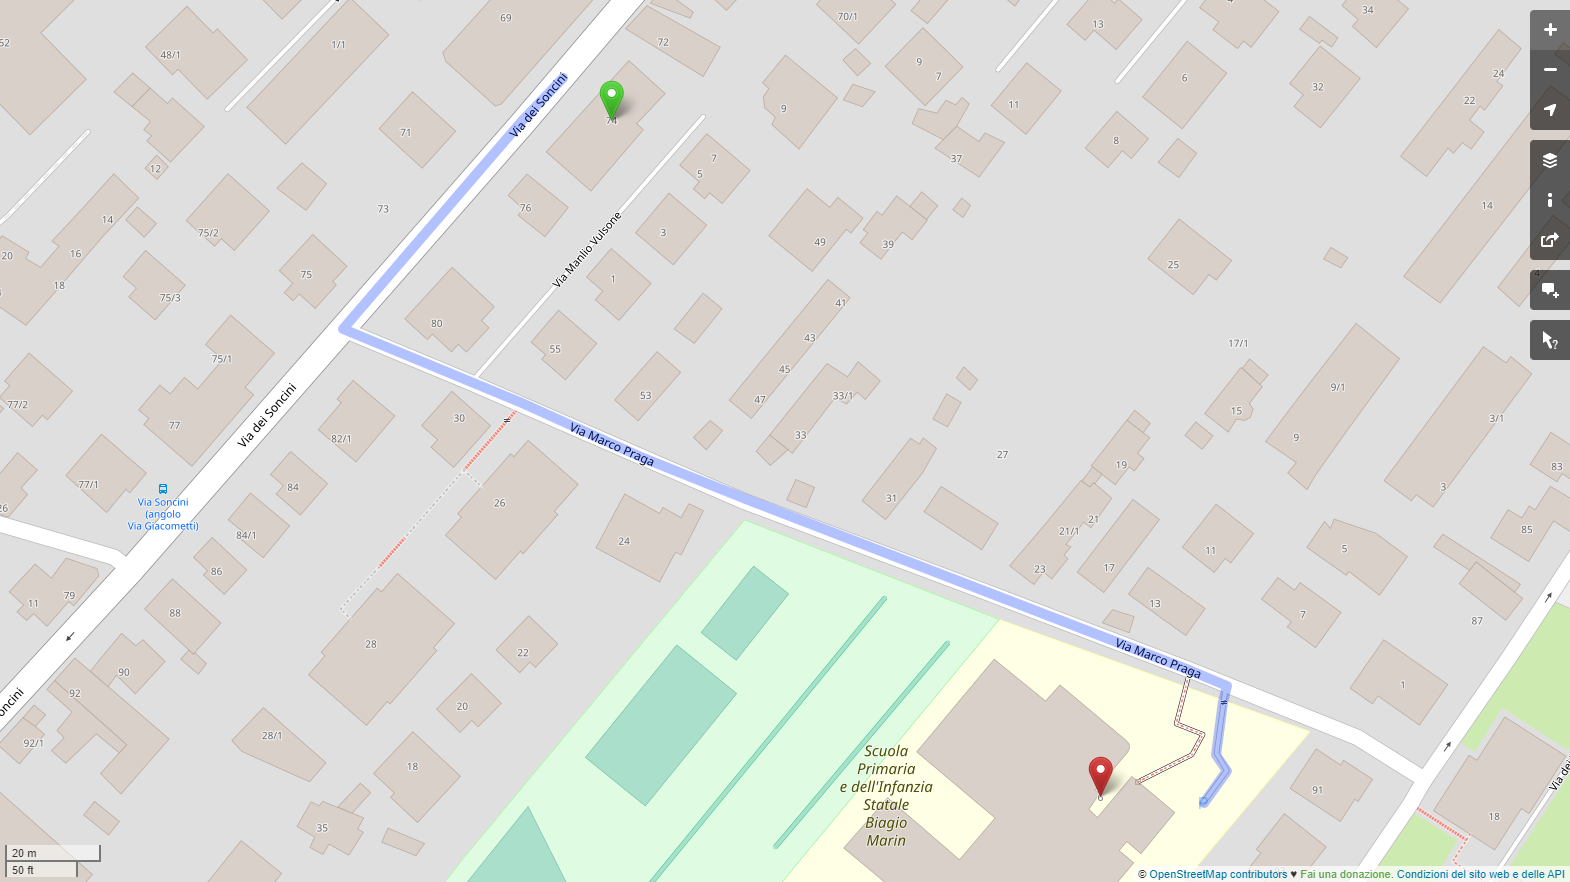
\includegraphics[scale=0.36]{figures/Distanza 7998556-7998442 v2}
    \end{figure}
    
\end{frame}

\begin{frame}{}

    \begin{figure}
        \centering
        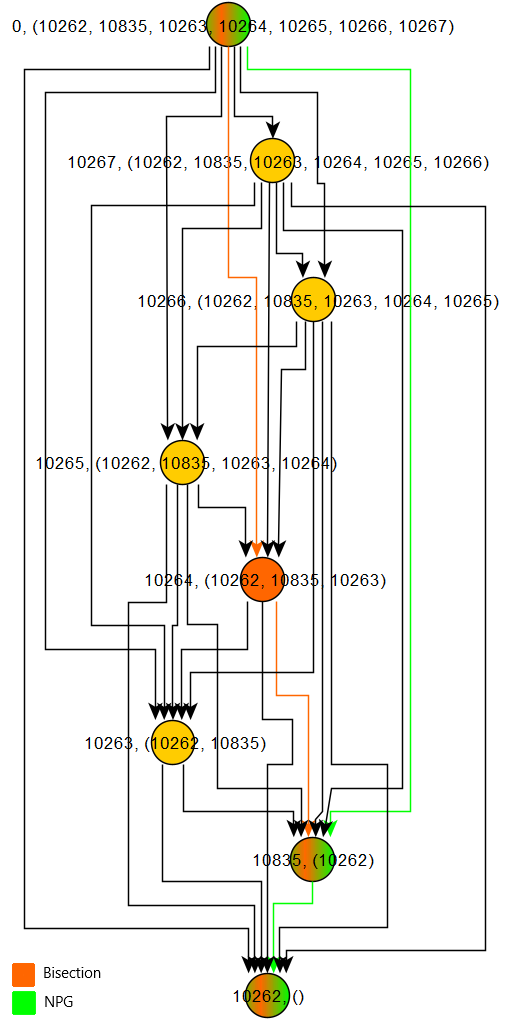
\includegraphics[scale=0.32]{figures/Policies_Bisection_NPG_3}
    \end{figure}
    
\end{frame}


\end{document}